% UC Merced  PhD Dissertation Template
% (UCSD Mathematics Dissertation Template is modified according to the UC Merced guidelines by Lasith Adhikari. Not responsible for any issues regarding modifications. You are welcome to add/update if there is any missing requirernment)
%
% Please read the comments in this file and make appropriate edits.
% NOTE: Always refer to the ``Preperation and Submission Manual for 
% Doctoral Dissertations and Masters Theses for 20**'', where 20** is 
% the year of your graduation, for officiation preparations guidelines.
%
% If you desire more control, please see the attached files:
%   * ucsd.cls -- Class file
%   * uct10.clo, uct11.clo, uct12.clo -- Configuration files for font sizes 10pt,11pt,12pt
%
% CHANGELOG:
%   * Original file adapted from brockman.tex by JRB and RMR
%     to work with ucsd.cls


\documentclass[11pt,oneside,chapterheads]{UCMerced}
% documentclass options: default is 11pt, oneside, final.
% fonts: 10pt, 11pt, 12pt -- are valid for UCSD dissertations (now UC Merced).
% sides: oneside, twoside -- note that two-sided theses are not accepted by OGS
% mode: draft, final -- draft mode switches to single spacing, removes hyperlinks,
%                       and places a black box at every overfull hbox (check these before submission).
% chapterheads -- include this if you want your chapters to read:
% Chapter 1
% Title of Chapter
%
% instead of
%
% 1 Title of Chapter


% Include all packages you need here.  Some standard options are suggested below.

% GEOMETRY - This will force the use of Letter paper.
% Many TeX installations default to A4 paper.  The formatting
% of the thesis class file requires Letter, else the margins
% will be wrong when you go to print it (and OGS will complain).
% If your TeX implementation is not setup for Letter paper, and
% you cannot change it, uncommenting the following line may fix 
% problem.
% \usepackage[paper=letterpaper]{geometry}

\usepackage{graphicx}

%% AMS PACKAGES - Chances are you will want some or all of these if writing a math dissertation.
\usepackage{amsmath, amscd, amssymb, amsthm}
\usepackage{multicol}
\usepackage{tabulary}
\usepackage{tabularx}
\usepackage{makecell}
\usepackage{pgfplots}
\usepackage{longtable}
\usepackage{url}
\usepackage{float}
\usepackage{subcaption}
\captionsetup[figure]{font=footnotesize}
\usepackage{epstopdf}
\epstopdfsetup{update} 
\usepackage{booktabs}
\usepackage{algorithm}
\usepackage{algorithmic}
\usepackage[Lenny]{fncychap}
\usepackage{pdfpages}
\usepackage{graphbox}

%--Additional packages--------------------------------------------------------------
\usepackage{mathtools}
\usepackage{arydshln}
\usepackage{epsfig}
\usepackage{framed}
\usepackage{bm}
\usepackage{palatino,verbatim}
\usepackage{indentfirst}
%-----------------------------------------------------------------------------------

%% LATIN MODERN FONTS (replacements for Computer Modern)
\usepackage{lmodern}
\usepackage[T1]{fontenc}



\usepackage{url}
\usepackage[colorlinks=true, pdfstartview=FitV, linkcolor=black, citecolor=black, urlcolor=black,plainpages=false,pdfpagelabels]{hyperref}
\usepackage{cleveref}
\usepackage[backend=biber,style=apa,sortcites=false,minnames=1,maxnames=3,maxbibnames=4]{biblatex}

\makeatletter
\DeclareCiteCommand{\fullcite}
{\defcounter{maxnames}{\blx@maxbibnames}%
\usebibmacro{prenote}}
{\usedriver
{\DeclareNameAlias{sortname}{default}}
{\thefield{entrytype}}}
{\multicitedelim}
{\usebibmacro{postnote}}
\DeclareCiteCommand{\footfullcite}[\mkbibfootnote]
{\defcounter{maxnames}{\blx@maxbibnames}%
\usebibmacro{prenote}}
{\usedriver
{\DeclareNameAlias{sortname}{default}}
{\thefield{entrytype}}}
{\multicitedelim}
{\usebibmacro{postnote}}
\makeatother


\addbibresource{EY_thesis.bib}
\let\cite\parencite

\theoremstyle{plain}% default
\newtheorem{theorem}{Theorem}[section]
\newtheorem{lemma}[theorem]{Lemma}
\newtheorem{proposition}[theorem]{Proposition}
\theoremstyle{definition}
\newtheorem{definition}{Definition}[section]

\begin{document}

\title{Flows of settling marine aggregates 
\\
and complex fluid rheology}
\author{Eunji Yoo}
\degreeyear{2023}
\degree{Doctor of Philosophy}  
\field{Applied Mathematics}

\numberofmembers{4} % |chair|  + |othermembers| (do not count co-chair) % change here
\chair{François Blanchette}
\cochair{Shilpa Khatri}

\memberone{Changho Kim}
\membertwo{Camille Carvalho (Institut National des Sciences Appliquées de Lyon)}
\memberthree{Ishan Srivastava (Lawrence Berkeley National Laboratory)}
% \memberfour{<COMMITTEE MEMBER 4>}




\begin{frontmatter}
\makefrontmatter % The title, copyright, and signature pages.

\tableofcontents
\listoffigures
\listoftables

%% DEDICATION
\begin{dedication}
    To my family, Dr. Dallerit 
    \\
    To my friends, Diversity 101 \& Susan   
    \\
    To my heavenly Father 
    \\
    I can do all things through Him who strengthens me.
    \\
    \hspace{65mm} - Philippians 4:13 
\end{dedication}

%% ACKNOWLEDGEMENTS
\begin{acknowledgements} 
    % Thanks to Francois and Shilpa, 
% \\
% and Michael
\end{acknowledgements}

%% Vita
% {
% \phantomsection
% \addcontentsline{toc}{chapter}{\protect\numberline{}Curriculum Vitae}%
% 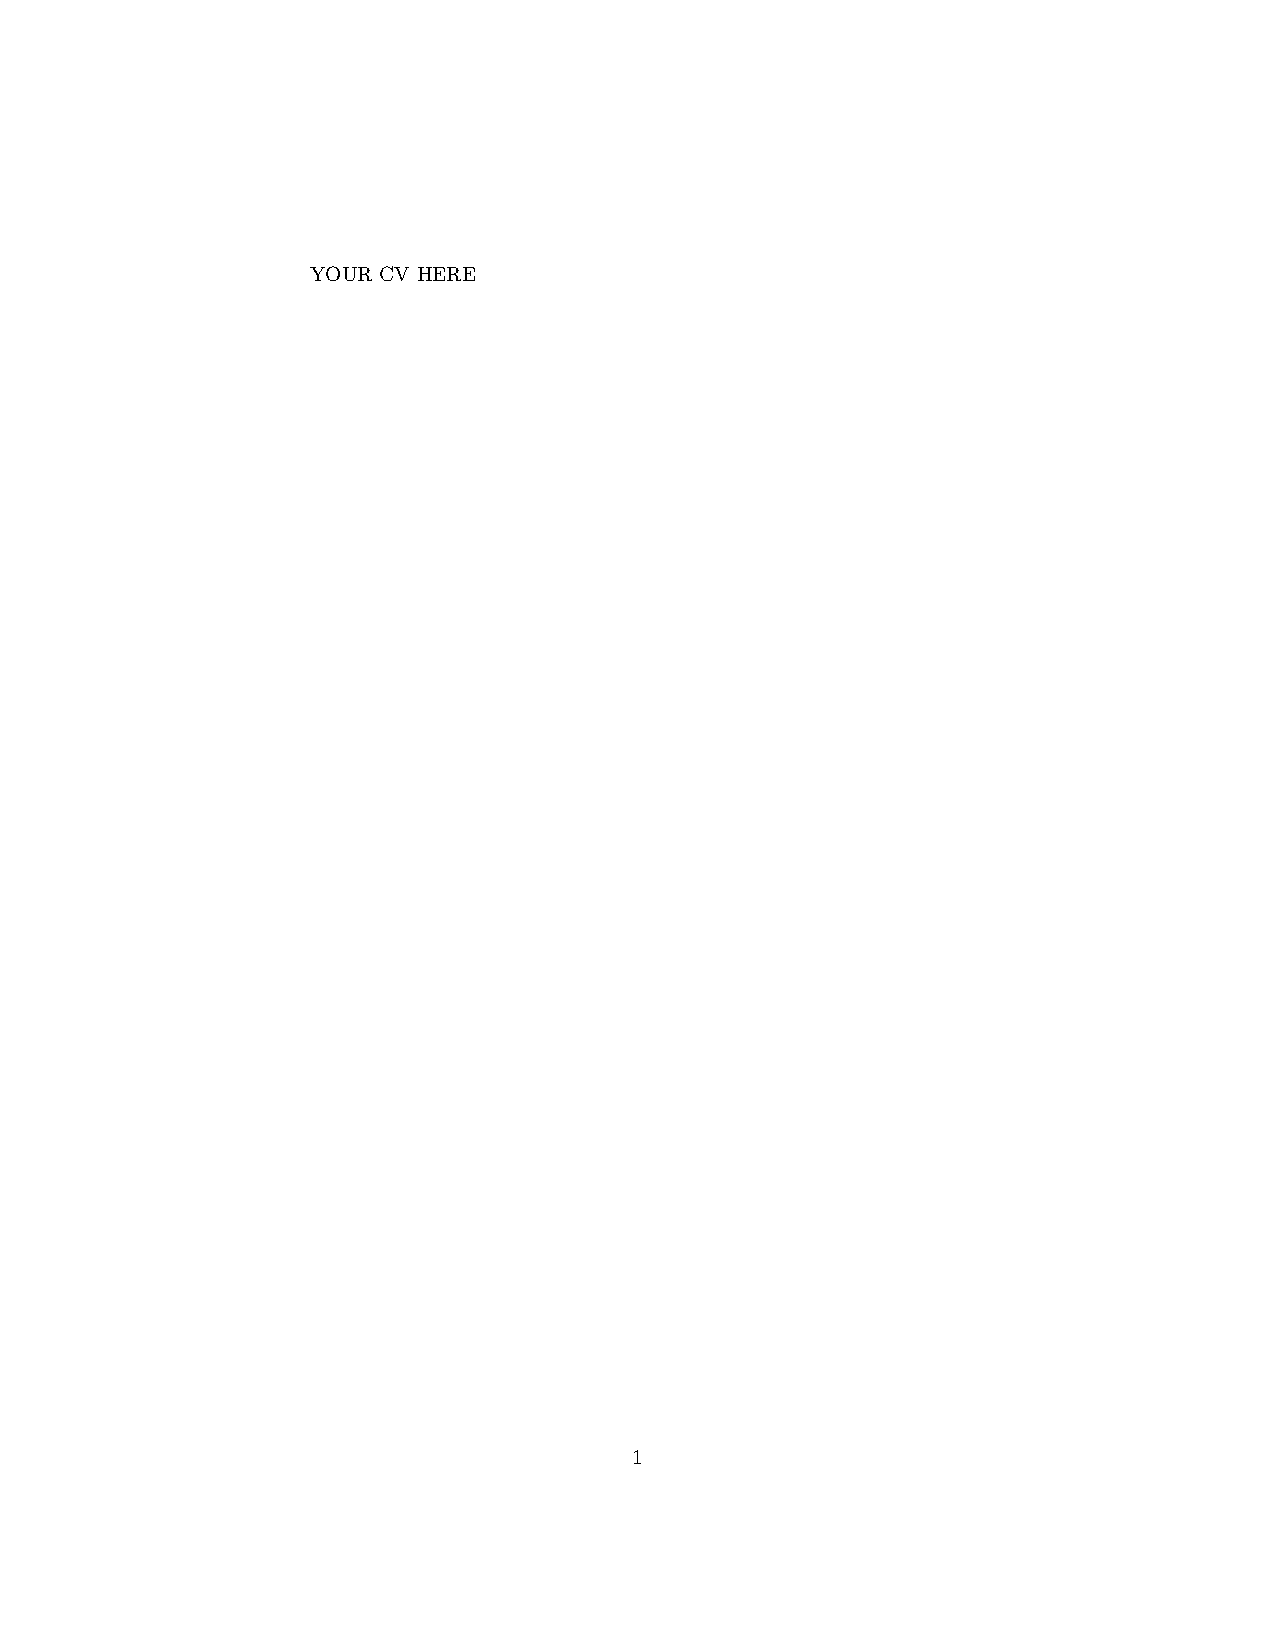
\includepdf[pages=1-,pagecommand={\thispagestyle{preliminary}}]{cv/cv.pdf}
% } 

%% Abstract
\begin{abstract}  
    ABSTRACT
\end{abstract}

\end{frontmatter}

%%% DISSERTATION
\chapter{Introduction}
\label{ch:intro}
% INTRODUCTION
Marine aggregates are randomly formed particles composed of organic and inorganic matters, such as phytoplankton, detritus, sediment, and fecal pellets \cite{jackson_simulation_1989}. Since these components stick together arbitrarily, a marine aggregates is often shown a fractal structure. 
These marine aggregates take in carbon dioxide (CO$_2$) during photosynthesis near the surface ocean and carry the dissolved carbon to the deep ocean. 
% The ocean absorbs $40 \%$ of the anthropogenically produced carbon dioxide (CO$_2$) from the atmosphere \cite{omand_sinking_2020}. 
This process removes CO$_2$ from the atmospheric carbon cycle \cite{honjo_understanding_2014}, and plays a role in regulating atmospheric CO$_2$ and climate changes which is one of the most significant environmental problems we face today. 
 \par
 It has been observed that larger sinking aggregates tend to accumulate in thin layers where the ambient fluid is density stratified \cite{alldredge_occurrence_2002}.The highly concentratedthin layers become biological hotspots for bacterial activity and animal feeding. It is ecologically important to understand the marine aggregates dynamics as they delay in settling.
\par
Our research is centered on computing the velocity field around settling marine aggregates and the forces acting on them. We do so using boundary integral equation (BIE) formulations. We construct marine aggregates using cubes to capture their fractal shape, as shown in Figure \ref{fig_cube10}. 
\begin{figure}[ht]
	\begin{center}
		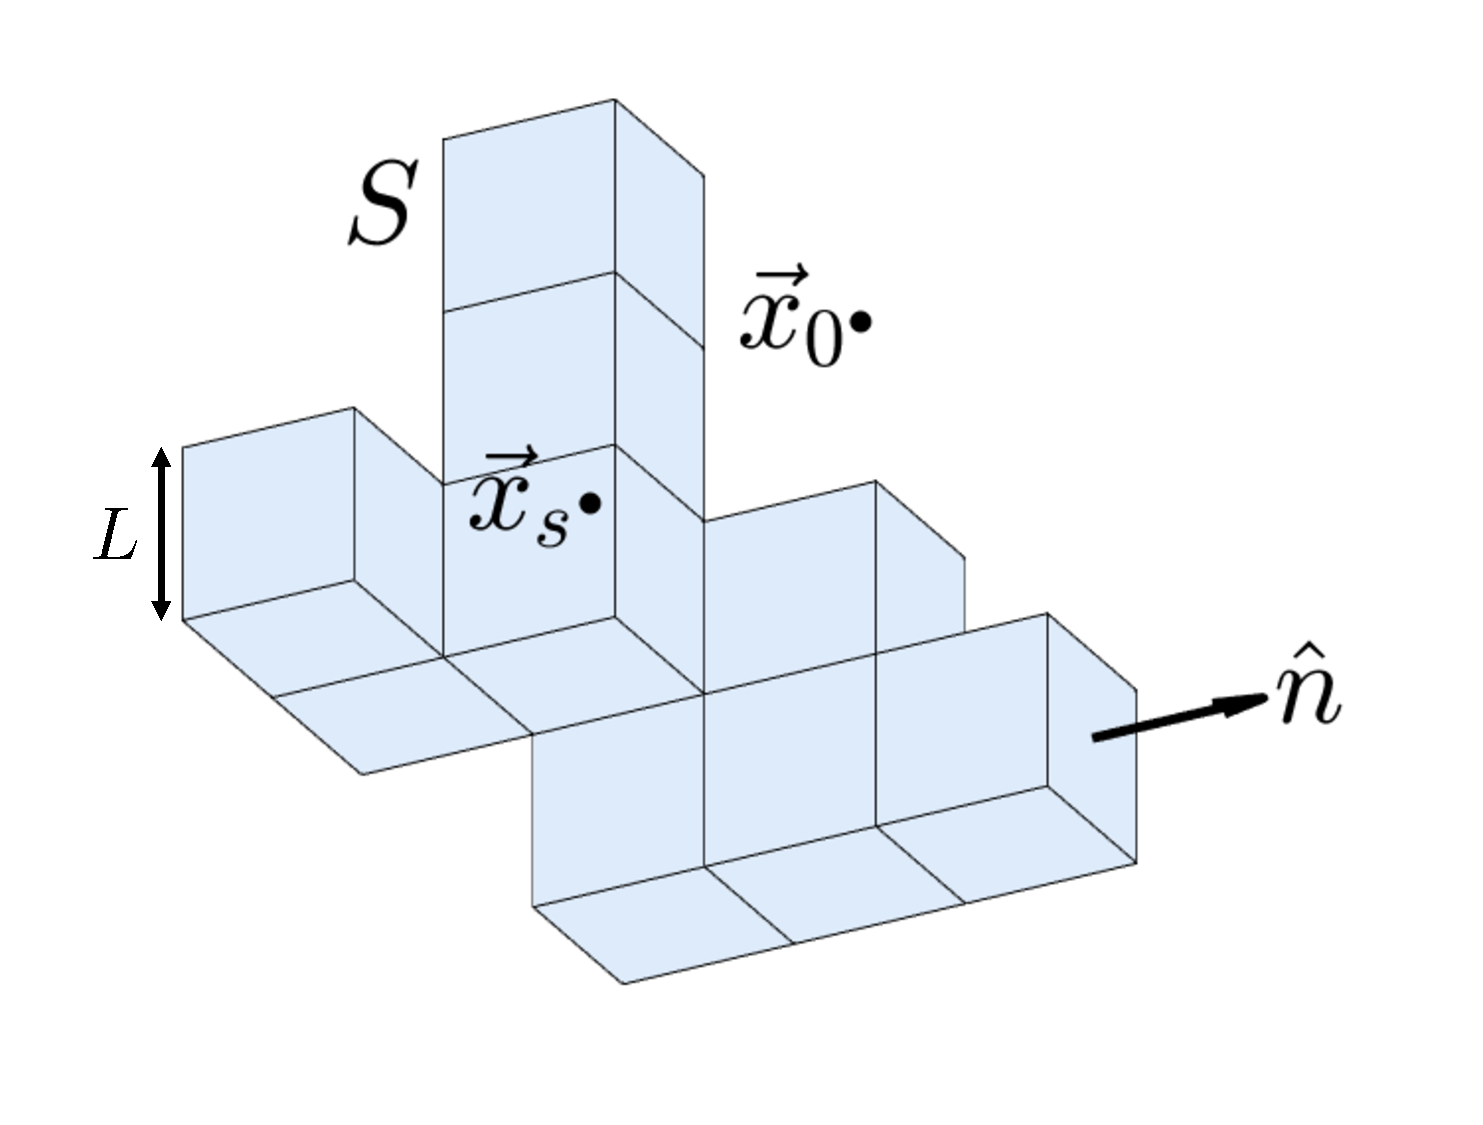
\includegraphics[scale=0.25]{figures/fig_cube10_CC.pdf}
	\end{center}
	\caption{Example aggregate model with 10 cubes. We denote $S$ as the particle surface and $\hat{n}$ as its normal. The vectors $\vec{x}_s$ and $\vec{x}_0$ represent points on and outside of $S$. }
	\label{fig_cube10}
\end{figure}

A detailed explanation of the modeling is in this chapter, section XX.
\par
{\color{red} Move the followings into each subsection.}
In chapter 2, we introduce the governing equations and the velocity solutions to the system. This includes the comparison of two BIE formulations. We then show the numerical methods for solving the velocity field and compuations of forces. We analyze the drag, torque, straining forces acting on the different sizes of aggregates with three types of background flows.
 To simulate concentration dynamics, we couple the velocity obtained using the BIE method with the advection-diffusion equation.
\par
In chapter 3, we consider a varying density fluid case. Due to the fluid density gradient, we modify the fluid momentum equation. We also derive the particular velocity solution in addition to the homogeneous solution. Since the new velocity solution includes a volume integral term which is computationally expensive to evaluate, we use the fast multipole method (FMM). In section XX, we give an introduction to the FMM and its open-source library. 
\par
{\color{blue} ADD DESCRIPTION OF CHAPTER 4 AND 5}
\section{Fluid momentum equations}
To describe the incompressible fluid motion that takes place around marine aggregatess, we consider the Navier-Stokes equations,
\begin{align}
\nabla \cdot \vec{u} = 0 
\label{eq_conserv_mass} \\
\rho 
\left( 
   \frac{\partial \vec{u}}{\partial t} + \vec{u}\cdot \nabla \vec{u}
\right)
  = \nabla \cdot \bar{\bar{\sigma}} +  \rho  \vec{g} ,
\label{eq_momentum_NS}
\end{align}
where $ \rho$ is fluid density (constant) and $\vec{u}, \ \vec{g}$ are fluid velocity and gravity vectors, respectively.
The first equation (\ref{eq_conserv_mass}) shows the conservation of mass and the equation (\ref{eq_momentum_NS}) describes the momentum conservation. 
We also introduce the stress tensor, $\bar{\bar{\sigma}}$ as 
\begin{equation}
   \bar{\bar{\sigma}} = -P \bar{\bar{I}} + {\tilde{\mu}} {\bm D},
   \label{eq_stress_tensor}
\end{equation}
where $P$ is fluid pressure and ${\tilde{\mu}}$ is fluid viscosity. Here, ${\bm D}$ is the symmetric strain rate tensor,
\begin{equation}
   \boldsymbol{D} = \frac{1}{2} \left( \nabla \vec{u} + (\nabla  \vec{u})^T \right).
   \label{eq_strain_rate}
   \end{equation}
Since seawater is Newtonian fluid, following the Newton's law of viscosity, the strain rate (\ref{eq_strain_rate}) becomes $\nabla \vec{u}$. This implies that we can re-write the momentum equation (\ref{eq_momentum_NS}) as
\begin{equation}
  \rho \left( 
   \frac{\partial \vec{u}}{\partial t} + \vec{u}\cdot \nabla \vec{u}
\right)
  = -\nabla P  + {\tilde{\mu}} \nabla^2 \vec{u}+  \rho  \vec{g} 
\end{equation}
For a typical seawater, it is reasonable to say $\rho \approx 1025 \text{kg/m}^3$ and ${\tilde{\mu}} = 1.2 \times 10^{-3}\text{kg}/\text{ms}$.
Also, the gravitaty vector is $\vec{g} = - g\hat{k} \approx -9.8$m/$s^2 \times (0,0,1)$ where $\hat{k}$ points in the vertical direction (upward). 
\par
 The momentum equation (\ref{eq_momentum_NS}) can be linearized for flows where inertial effects are small. 
To estimate the size of the main forces at play, we consider a radius of marine aggregate, $R_a \approx 5 \times 10^{-5}$(m) and the reference Stokes settling speed of an aggregate,
\begin{equation}
    U_s =  \frac{gR_a^2}{{\tilde{\mu}}} (\rho_a-\rho) \approx 3.8 \times 10^{-4} ({\text{m/s}}),
	\label{eq_U_s}
\end{equation}
where $\rho_a \approx 1400\text{kg/m}^3$ is the aggregate mass density. 
When we non-dimensionalize the momentum equation using the length scale, $R_a$ and velocity, $U_s$, we can obtain the following equation:
\begin{equation}
	\left(\frac{\rho U_s R_a}{{\tilde{\mu}}} \right) 
   \left( 
   \frac{\partial \vec{u}'}{\partial t'} + \vec{u}'\cdot \nabla' \vec{u}'
\right)
 = {\nabla'}^2 \vec{u}' - \nabla' P' +  \vec{g}',
 \label{eq_NS_moment_noD}
\end{equation}
where we find and compute the Reynolds number (Re),
\begin{equation}
	\text{Re} = \frac{\rho U_s R_a}{{\tilde{\mu}}} \approx 10^{-2}
	\ll 1.
\end{equation}
Note that we use the prime symbol to represent a dimensionless value.
Since we have fairly small Reynolds number, we may neglect the inertial effects, limiting the left-hand side of equation (\ref{eq_NS_moment_noD}) to zero,
\begin{equation}
   {\nabla'}^2 \vec{u}' - \nabla' P' +  \vec{g}' = 0.
\end{equation}
In this thesis, we therefore consider the following Stokes equations, writing back with dimensions, to describe the fluid flow around the settling aggregates,
 \begin{align}
	\nabla \cdot \vec{u}  = 0  
	% \label{eq_conti2}
	\nonumber \\
	{\tilde{\mu}} \nabla^2 \vec{u}    - \nabla P\ + \rho  \vec{g} = 0.
	\label{eq_stokes2}
\end{align}
The solutions of the system of equations are the fluid velocity, $\vec{u}$, and pressure, $P$. In general, pressure does not induce motion. We see the pressure at rest, denoted as $P_s$, contains the pressure of gravity,  $P_s(\vec{y}) = \rho \vec{g} \cdot \vec{y}$, where $\vec{y} \in \mathbb{R}^3$ is a point in the fluid. Using this static pressure term, we introduce the dynamic pressure $P_d$, defined as 
\begin{equation}
   P_d(\vec{y}) = P(\vec{y}) - P_s(\vec{y}) = P(\vec{y}) - \rho \vec{g} \cdot \vec{y}.
   \label{eq_def_Pd}
\end{equation}
By substituting the expression (\ref{eq_def_Pd}), we obtain
\begin{align}
	\nabla \cdot \vec{u}  = 0  
	% \label{eq_conti2}
	\nonumber \\
	{\tilde{\mu}} \nabla^2 \vec{u}    - \nabla P_d = 0.
	\label{eq_stokes3}
\end{align}
In our simulation, we focus on the velocity field and hydrodynamic forces around the marine aggregate model. 

{\color{red} ADD FIGURE TO EXPLAIN NOTATIONS.}
% {\color{blue}WHY NO PRESSURE?}
%
%===SECTION 2.2=========================================
\section{Boundary integral equation (BIE) formulations} 
For our simulations, we consider a large fluid domain compared to the size of an aggregate, having zero fluid velocity at infinity. We also treat our aggregate surface as a solid. Although marine aggregates are porous, the solid boundary condition is reasonable to apply due to their low permeability. 
% These conditions allow us to eliminate one of the integrals. The detailed derivation is provided in section 2. 
This condition prevents a flow through the aggregate, acting like a solid particle. For this reason, any flow inside of the aggregate is neglected in the remainder of this thesis.  
\par
The fundamental solution $\vec{u}(\vec{y})$, to the Stokes equations, (\ref{eq_stokes2}), at any point $\vec{y} \in \mathbb{R}^3$ that is outside of an object boundary, $S(\vec{x})$, is
% around a solid object is expressed, using the stress vector, $\vec{f}$, 
\begin{equation}
   \vec{u}(\vec{y}) =
	- \frac{1}{8 \pi {\tilde{\mu}}} \int_S  \vec{f}(\vec{x}) \cdot \bar{\bar{G}}(\vec{x},\vec{y}) \ \text{d}S(\vec{x}) 
+ \frac{1}{8 \pi} \int_S
\vec{u}(\vec{x}) \cdot  \bar{\bar{T}}(\vec{x},\vec{y})  
\cdot \hat{n} ( \vec{x})
\ \text{d}S(\vec{x}),
\label{eq_BIE}
\end{equation}
where  $\vec{f}(\vec{x})$ is the stress vector that describes a point force at $\vec{x} \in S$ \cite{pozrikidis_boundary_1992}. Here, the second order tensor in equation (\ref{eq_BIE}) is the Green's function,  $\bar{\bar{G}}(\vec{x},\vec{y})$,
\begin{align}
  \bar{\bar{G}}(\vec{x},\vec{y}) =   
  \frac{\bar{\bar{I}}}{||\vec{x}-\vec{y}||} + \frac{(\vec{x}-\vec{y})(\vec{x}-\vec{y})}{||\vec{x}-\vec{y}||^3},
  \label{eq_stokeslet}
  \end{align}
  and the stress tensor, $\bar{\bar{T}}(\vec{x},\vec{y})$ , associated with the Green's function of the Stokes equations,
  %
  \begin{align}
  \bar{\bar{T}}(\vec{x},\vec{y}) = 
  -6\frac{(\vec{x}-\vec{y})(\vec{x}-\vec{y}) (\vec{x}-\vec{y})}{||\vec{x}-\vec{y}||^5},
  \label{eq_stresslet}
  \end{align}
where $\| \cdot \|$ is the $L^2$ norm. 
Note that $ \bar{\bar{G}}(\vec{x},\vec{y})$ and $ \bar{\bar{T}}(\vec{x},\vec{y}) $ are called  the {\textit{Stokeslet}} and {\textit{Stresslet}}, respectively.
The first integral distribution on the right-hand side of equation (\ref{eq_BIE}) is called the \textit{single-layer potential} and the second one is called the \textit{double-layer potential}. 
\\
{\color{red} ADD THE PHYSICAL MEANING OF THESE TENSORS - FLOW DUE TO A POINT FORCE F}
\par
To compute the velocity at a point on the surface $S$, i.e., $ \vec{x}_s \in S$, we use 
\begin{equation}
   \vec{u}(\vec{x}_s) = - \frac{1}{4 \pi {\tilde{\mu}}} \int_S  \vec{f}(\vec{x}) \cdot \bar{\bar{G}}(\vec{x},\vec{x}_s) \ \text{d}S(\vec{x}) 
+ \frac{1}{4 \pi} 
\int_S
\vec{u}(\vec{x}) \cdot  \bar{\bar{T}}(\vec{x},\vec{x}_s)  
\cdot \hat{n} ( \vec{x})
\ \text{d}S(\vec{x}).
\label{eq_BIE_onS}
\end{equation}
Depending on the fluid domain characteristics and/or type of the object's surface, we can simplify the fundamental equation (\ref{eq_BIE}).


\section{Non-Newtonian fluid}
% Main difference between Newtonian vs Non-Newtonian. Explain the yield stress. Basic idea of rheology, and importnace of the secondary flow we want to capture.
We now turn our attention to a non-Newtonian fluid. This topic is added to my thesis as an extension of one summer internship at the Lawrence Berkeley National Lab in 2022. 
\par
A non-Newtonian fluid shows many interesting behaviors quite different than Newtonian fluids. It has variable viscosity that changes the state of a fluid under a particular pressure, i.e., the viscosity term,${\tilde{\mu}}$ in the stress tensor (\ref{eq_stress_tensor}) is not constant; rahter it is a function of the shear rate ($\dot{\gamma}$), that is
\begin{equation}
   \dot{\gamma} = \left| 
   {\boldsymbol{D}}
   \right|.
\end{equation}
Due to this varying viscosity, the constitutive behavior of non-Newtonian fluids is highly complex. They show intriguing phenomena such as shear thickening, shear thinning, jamming, shear banding, and normal stress differences. This broad class of fluids encompasses various materials of industrial and natural importance, such as granular fluids, polymeric fluids, gels, and suspensions. Complex fluids exhibit two phases as responses to applied stress. This thesis examines the time-dependent coexistence between a fluid's solid and liquid states: the study for this particular fluid type is called {\textit{rheology}}. As the viscosity of a non-Newtonian fluid can be a function of the shear rate, a defining feature of many complex fluids is the presence of yield stress: for an insufficiently stressed material, they behave like an elastic solid, but once the yield stress is exceeded, they flow like a fluid. 
% \begin{figure}[h]
% 	\begin{center}
% 		\includegraphics[scale=0.2]{figures/fig_Rheology_of_time_independent_fluids.pdf}
% 	\end{center}
%    \caption{Rheology graph - need to change}
%     %https://link.springer.com/referenceworkentry/10.1007/978-0-387-92897-5_143 
% 	\label{fig_rheology}
% \end{figure}
\par
Determining one's yield stress is critical to understand rheological behavior accurately. Typically, the stress for a complex fluid can be computed as,
\begin{equation}
   \boldsymbol{\tau} = \mu(\dot{\gamma}) \boldsymbol{D}.
\end{equation}
It was brought to our attention that there are characteristics that could be neglected when we consider the stress linear in $\boldsymbol{D}$. For instance, curvature in free-surface flows, anomalous stress profile in cylindrical Couette flows, or negative rod climbing effect (Weissenberg effect). We thus propose to implement the computational tools to study these secondary flow using the following stress tensor expression:
\begin{align}
  {\bm  \tau}
  =  \ &\mu_1 {\bm D} 
  + \mu_2  \left[ {\bm D}^2  - \frac{\text{tr}\left({\bm D}^2\right)}{3}{\bm I} \right]
  \nonumber \\
  & + \kappa_1 \frac{{\bm D}}{|{\bm D}|} 
  + \kappa_2  \left[ \frac{{\bm D}^2}{|{\bm D}|^2}  
  - \frac{\text{tr}\left({\bm D}^2\right)}{3|{\bm D}|^2}{\bm I} \right].
\end{align}
The terms $\mu_i$ and $\kappa_i$ ($i, j = 1,2,$)coefficients represent the shear rate-dependent and rate-independent contributions, respectively, to the total stress.
\par
With a constitutive rheology code, we can capture such complex continuum hydrodynamics. We thus consider both shear stress rate and the pressure onto the materials of interest as the sources of the yield stress. 
We use AMReX framework, developed at LBNL, NREL, and ANL, to solve flow motion. We implement the granular material viscosity computation in \verb+incflo+, which is an AMReX-based code for modeling the variable density incompressible Navier-Stokes equations without subcycling in time.





\chapter{Settling marine aggregates in a homogeneous fluid}
\label{ch:2}
Chapter 2

%% Add more chapters here if necessary

\chapter{Settling marine aggregates in a stratified fluid}
\label{ch:3}
%some-literature review


In the last few decades, several scientists have modeled the dynamics and ecological impact of marine aggregates~\cite{jackson_aggregation_1998, kiorboe_mechanisms_2002}. 
Their effects on bacterial transport~\cite{jackson_simulation_1989} and algal bloom~\cite{jackson_model_1990} have been described in models that use simplified descriptions of the aggregates' settling speeds. Moreover, accumulation of aggregates in thin layers where the ambient fluid is stratified has been reported~\cite{macintyre_accumulation_1995, alldredge_occurrence_2002} and more recently modeled experimentally~\cite{prairie_delayed_2013}, analytically~\cite{camassa_retention_2013}, and computationally~\cite{panah_simulations_2017}. 
Understanding marine aggregate formation, settling speed, and persistence of these thin layers is ecologically important. 
Therefore, in this chapter, we discuss the dynamics of settling marine aggregates in a density-stratified fluid. 
%--------------------------------------------------------
\section{Governing Equations}
In this chapter, instead of constant density $\rho$, as in Chapter 2, we suppose that the background fluid density varies linearly in the vertical direction,
\begin{equation}
\rho_{bg}(z) =  \rho_0 \left(1 - \gamma z \right),
\label{eq_rho_bg}
\end{equation}
where $\rho_0$ is the fluid density where the aggregate's center of mass is located at rest initially and $\gamma > 0$ is constant.
Over time, perturbations, $C(\vec{y},t)$, occur due to the settling motion due to non-homogeneous fluid. More specifically, we define $C$ as the concentration difference between the initial value and time $t$.
From this, we can establish the fluid density variation over time,
\begin{equation}
	\rho(\vec{y},t ) 
	= \rho_{bg}(z) +  \alpha \rho_0 C(\vec{y},t) 
	 = \rho_0 \left( 1 - \gamma z  + \alpha  C(\vec{y},t) \right),
\label{eq_density}
\end{equation}
where the non-zero constant $\alpha$ depends on the type of solute. We provide the schematic of the perturbation effect on the top of the background fluid density in Figure~\ref{fig_stratification_schematics}.
\begin{figure}[ht]
	\begin{center}
	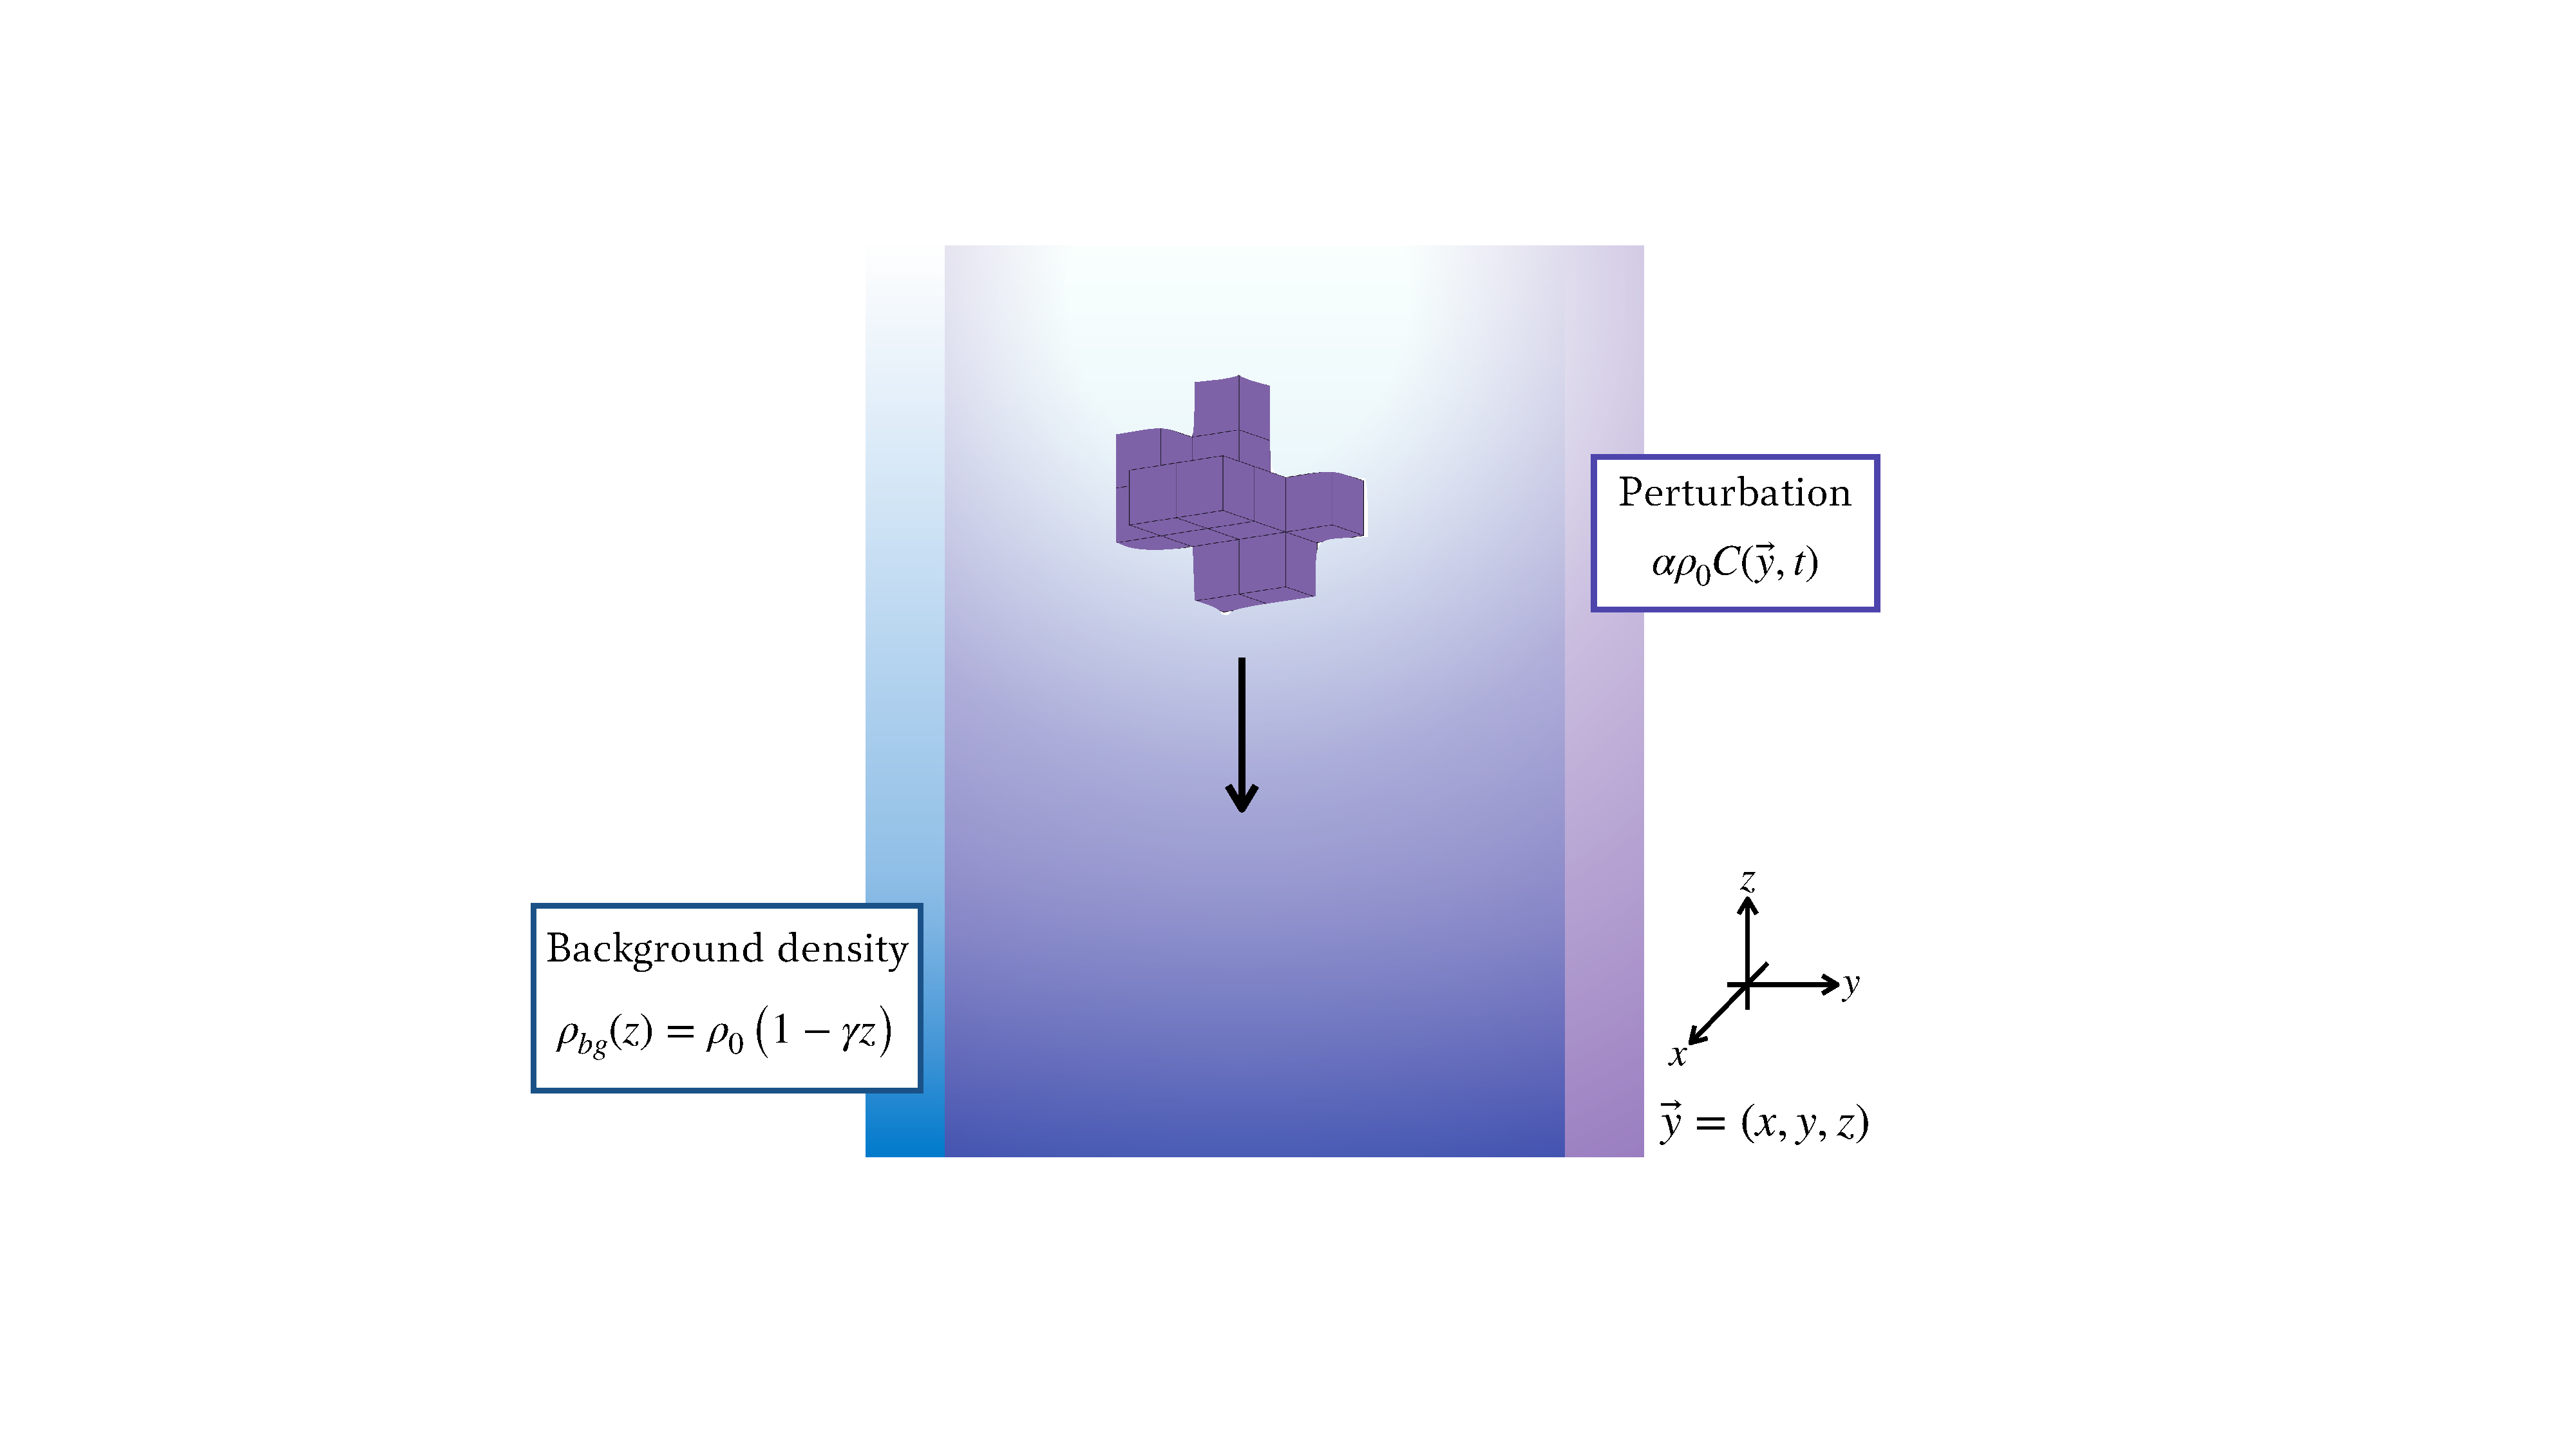
\includegraphics[scale=0.4]{./figures/fig_stratification_schematics}
	\caption{Description of fluid density stratification.}
	\label{fig_stratification_schematics}
	\end{center}
\end{figure}
The non-constant density $\rho(\vec{y},t)$ changes the momentum equation from (\ref{eq_stokes3}) to 
		 \begin{equation}
		\ \tilde{\mu}\nabla^2 \vec{u}(\vec{y})
		- \nabla P_d (\vec{y}) \ + \  
		 \rho_0 \alpha C(\vec{y},t) \vec{g} =0 , 
	\label{eq_extra_C}
	\end{equation}
	where $P_d$ is the dynamic pressure, defined as
\begin{equation}
	P_d (\vec{y})
	 = P (\vec{y}) \ - \int \rho_{bg}(z) g   \textrm{d}z.
	\label{eq_Pd}
\end{equation}
To take the density perturbation of the ambient fluid into account, we find a particular solution to the momentum equation (\ref{eq_extra_C}). Once we have it, simple addition to the homogenous solution gives the entire solution due to the linearity of the system. 
\par
% \subsection{Particular solution to Stokes equations with the stratification}
%----------------------------------------------------------------------
To derive a particular solution, we consider the singularly forced Stokes problem~\cite{pozrikidis_boundary_1992},
\begin{equation}
	\ \tilde{\mu} \nabla^2 \vec{u}(\vec{y})
	- \nabla P (\vec{y})
	+\vec{q} \ \delta \left(\vec{x} - \vec{y} \right) =0,
\label{eq_single_stokes}
\end{equation}
where $\vec{q}$ is an arbitrary constant vector, $\vec{x}$ is an arbitrary point in fluid domain, and $\delta$ is the three-dimensional delta function.
The problem (\ref{eq_single_stokes}) 
describes the effect coming from a singular force applied at $\vec{y} = \vec{x}.$
The fundamental solution to equation (\ref{eq_single_stokes}) coupled with the continuity equation (\ref{eq_conserv_mass}) are
\begin{equation}
	\vec{u} (\vec{y}) = \ \frac{1}{8\pi \tilde{\mu}}  \bar{\bar{G \ }}(\vec{x}, \vec{y})
	\cdot  \vec{q}
\label{eq_fund_u}
\end{equation}
\begin{equation}
	P (\vec{y}) = \ \frac{1}{4\pi }  
	\frac{\vec{x} - \vec{y}}{\| \vec{x} - \vec{y}\|^3}
	\cdot  \vec{q},
\label{eq_fund_p}
\end{equation}
where the kernel $\bar{\bar{G \ }}$ is the \textit{Stokeslet}, introduced in Chapter 1, equation (\ref{eq_stokeslet}).
This implies that the solutions (\ref{eq_fund_u}) and (\ref{eq_fund_p}) satisfy equation (\ref{eq_single_stokes}) as
\begin{equation}
	\ \tilde{\mu} \nabla^2 
	\biggl( \frac{1}{8\pi \tilde{\mu}}  \bar{\bar{G \ }}(\vec{x}, \vec{y})
	\cdot  \vec{q} \biggr)
	- \nabla \biggl(\ \frac{1}{4\pi }  
	\frac{\vec{x} - \vec{y}}{\| \vec{x} - \vec{y}\|^3}
	\cdot  \vec{q} \biggr)
	+ \vec{q} \ \delta \left(\vec{x} - \vec{y} \right)
	=0.
\label{eq_single_stokes_sub}
\end{equation}
When we multiply by $ C(\vec{x},t) $ on both sides and integrate the entire equation over the domain, $V(\vec{x})$, we get
\begin{equation}
	\int_{V}
	\biggl[
	\ \tilde{\mu} \nabla^2 
	\biggl( \frac{ \bar{\bar{G \ }}(\vec{x}, \vec{y})
	\cdot  \vec{q}}{8\pi \tilde{\mu}}  \biggr)
	C(\vec{x}, t)
	-
	\nabla \biggl( 
	\frac{(\vec{x} - \vec{y}) \cdot  \vec{q} }{4 \pi \| \vec{x} - \vec{y}\|^3}
	\biggr)
	C(\vec{x}, t)
	+ \vec{q} \ \delta \left(\vec{x} - \vec{y} \right)
	C(\vec{x}, t)
	\biggr]
	\ \textrm{d}V(\vec{x}) = 0 .
\label{eq_single_stokes_sub2}
\end{equation}
Note that the operator $\nabla$ is linear and describes derivatives in $\vec{y}$. We are able to switch the order with the integral operator as follows,
\begin{equation}
	\tilde{\mu} \ \nabla^2 
	\int_{V}
	\biggl( \frac{\bar{\bar{G \ }}(\vec{x}, \vec{y})
	\cdot  \vec{q} }{8\pi \tilde{\mu}}  \biggr)
	C(\vec{x}, t)
	\ \textrm{d}V(\vec{x})
	-
	\nabla 
	\int_{V}
	\biggl(
	\frac{	C(\vec{x}, t)(\vec{x} - \vec{y})\cdot  \vec{q} }{4 \pi \| \vec{x} - \vec{y}\|^3} \biggr)
	\ \textrm{d}V(\vec{x})
	+\vec{q} C(\vec{x}, t) = 0 .
\label{eq_single_stokes_sub3}
\end{equation}
By choosing $\vec{q} = \rho_0 \alpha \vec{g}$, we can find a particular solution to our modified Stokes momentum equation, (\ref{eq_extra_C}),
\begin{equation}
	\vec{u} (\vec{y}) =
	 \frac{\rho_0 \alpha }{8\pi \tilde{\mu}}
	\int_{V}  \bar{\bar{G \ }}(\vec{x}, \vec{y})
	\cdot  C(\vec{x}, t) \vec{g} 
	\ \textrm{d}V(\vec{x}).
\label{eq_fund_soln_unit}
\end{equation}
\begin{equation}
	P(\vec{y}) = 
	\frac{\rho_0 \alpha }{4\pi }  
	\int_{V}
	\frac{\vec{x} - \vec{y}}{\| \vec{x} - \vec{y}\|^3}
	\cdot 
	C(\vec{x}, t) \vec{g} 
	\ \textrm{d}V(\vec{x}).
\label{eq_fund_soln_p}
\end{equation}
The entire velocity solution, thus, becomes
\begin{equation}
	 \vec{u} \left(\vec{y}, t \right) =
	 - \frac{1}{8 \pi \tilde{\mu}} \int_{S}  
		 \vec{f}(\vec{x}) 
		 \cdot \bar{\bar{G \ }} (\vec{x},\vec{y}) 
		 \ \textrm{d}S(\vec{x})
	+ \frac{ \rho_0 \alpha  }{8\pi \tilde{\mu}} \int_V  C \left(\vec{x},  t \right) \vec{g} \cdot 
	\bar{\bar{G \ }}(\vec{x}, \vec{y} ) 
	\ \text{d}V(\vec{x}).
\label{eq_vel_HP}
\end{equation}
As we see, the velocity at a point $\vec{u}(\vec{y},t)$ is now dependent on space and time compared to the homogeneous fluid case. We can update the velocity field in time by coupling the solution (\ref{eq_vel_HP}) with the advection-diffusion equation (\ref{eq_ad_diff_nonD}) to model the solute perturbation, $C$.
 
%------------------------------------------------------------------
\subsection{Force balance}
\label{sec:force_balance}
\par
Since the velocity of the aggregate is no longer constant in time, we need to solve for it.
Specifically, we now need to solve for the translational and angular velocity, $\vec{U}_a$ and $\vec{\Omega}$, respectively, by prescribing the total body force and total torque from the fluid on the aggregate.
To close the system of equations, we prescribe the total drag force, $\vec{F}_o$, and total torque, $\vec{Q}_o$. 

First, we know that the total drag is the sum of the stress, $\vec{f}$,
\begin{equation}
	 \vec{F}_o = \int_S \vec{f} (\vec{x}) \ \textrm{d}S 
	= - \int_S \left[ 
	 - \left( P -  \int \rho_{bg}(z) g \ \textrm{d}z \right) \bar{\bar{I \ }} 
	 + \tilde{\mu} \left( \nabla \vec{u} + (\nabla \vec{u})^{T} \right)
	 \right] \cdot \hat{n} \ \textrm{d}S (\vec{y}).
\label{eq_Fo}
\end{equation}
To impose the total drag (\ref{eq_Fo}), we observe the right-hand side of equation (\ref{eq_Fo}) includes the buoyancy force, $\vec{F}_{b}$. 
As we work in the Stokes regime, the net force on the aggregate must be zero, so we have
\begin{equation}
	\vec{F}_o (t)+\vec{F}_g(t) + \vec{F}_b = \vec{0},
	\label{eq_Full_Force}
\end{equation} 
where the gravity force acting on the aggregate, $\vec{F}_g$, can be expressed as
\begin{equation}
	\vec{F}_g = \rho_a V_a \vec{g}, 
	\label{eq_F_gravity}
\end{equation}
with aggregate density $\rho_a$ and volume $V_a$. 
To calculate the aggregate density, $\rho_a$, we consider aggregate porosity, $\phi$, that is $ 0 \leq \phi \leq 1$.
 We then define the density of an aggregate as 
\begin{equation}
	\rho_a  = \phi \rho_{f} + (1-\phi) \rho_{s},
	\label{eq_rho_a}
\end{equation}
where $\rho_{f}$ and $\rho_s$ are the density of the fluid and solid portion of the aggregate, respectively. To obtain the fluid portion of the aggregate density, we take an average of the fluid density where the aggregate is located,
\begin{equation}
	\rho_{f}(t) = \frac{1}{V_a}\int_{V_a} \rho(\vec{x}, t) \  \textrm{d}V(\vec{x}))
\end{equation}
We here consider the solid part of the aggregate density as $\rho_s \approx 1400 $kg$/$m$^3.$ 
We also set the porosity to $\phi = 0.95$.
Meanwhile, we find the buoyancy force, $\vec{F}_b$, from equation (\ref{eq_Fo}),
\begin{equation}
 \vec{F}_b =	  -  \int_S \left( 
	   \int \rho_{bg}(z) g \ \textrm{d}z 
	 \right) \bar{\bar{I \ }}  \cdot
	\hat{n} \ \textrm{d}S (\vec{y}).
\label{eq_F_buoyancy}
\end{equation}

For the total torque, we use the form (\ref{eq_torquebal}), and set the value to zero,
\begin{equation}
	\vec{Q}_o =\int_S \vec{f}\times (\vec{x} - \vec{x}_{cm}) \ \textrm{d}S =  \vec{0}.
\label{eq_Qo}
\end{equation}
 Note that this does not imply that the aggregate is not rotating. 
%--------------------------------------------------
\subsection{Perturbation variation}
As the aggregate settles, the concentration, and therefore the fluid density, changes
\begin{equation}
	\frac{\partial \rho(\vec{y},t)}{\partial t}
	+ \vec{u}(\vec{y}) \cdot \nabla \rho(\vec{y},t)
	 = D \nabla^2 \rho(\vec{y},t),
\label{eq_AD_rho}
\end{equation}
where $D$ is the diffusion coefficient.
By applying the relationship between fluid density $\rho$ and the concentration perturbation $C$ from equation (\ref{eq_density}), we can re-write the equation (\ref{eq_AD_rho}) in terms of $C$, 
\begin{equation}
	\frac{\partial C(\vec{y},t)}{\partial t}
	+ \vec{u}(\vec{y}) \cdot \nabla C(\vec{y},t)
	 = D \nabla^2 C(\vec{y},t)
	 + \frac{\gamma}{\alpha}\vec{u}(\vec{y})  \cdot \hat{k}.
\label{eq_AD_C}
\end{equation}
Note that the advection-diffusion equation for $C$ contains an additional source term that
depends on the vertical component of the fluid velocity.

%------------------------------------------------------------------
\section{Dimensional analysis}
To facilitate further analysis, we non-dimensionalize our new equations. We mainly use the same parameters we introduced in section~\ref{section3}, equations (\ref{eq_nonD}), in addition to the following dimensionless parameters:
\begin{equation}
	C= C_{max} C'
\hspace{7mm}
\rho = \frac{\tilde{\mu}  }{{U_s} R_a}  \rho', 
\end{equation}
In this chapter, the Stokes settling speed $U_s$, defined in equation (\ref{eq_U_s}), becomes
\[
U_s = \frac{g  R_a^2}{\tilde{\mu}}(\rho_s - \rho_0)(1-\phi),
\] 
since we consider the porosity of an aggregate as (\ref{eq_rho_a}).
% Note that the Reynolds number is approximately 0.03.
 % Here $\rho_a$ is the density of aggregate.
For the scale of the perturbation, $C$, we introduce the maximum density difference of the background density profile in the fluid domain at the initial time, i.e., 
\begin{equation}
C_{max} = 
\frac{1}{\alpha \rho_0}
\left|
\max_{\vec{x}\in V} \left(\rho_{bg}(z)  \right)
\ - \min_{\vec{x} \in V} \left(\rho_{bg}(z)  \right) \right|.
\end{equation}
\par
We first derive the dimensionless modified Stokes momentum equation, using primes to indicate dimensionless variables,
\begin{equation}
	{\nabla'}^2  \vec{u}'(\vec{y})
	= \nabla {P_d}'(\vec{y}) \ - \  
	\frac{\alpha \rho_0  C_{max}}{(\rho_s - \rho_0)(1-\phi)}  C'\left(\vec{y},t \right)   \hat{k},
\label{eq_extra_C_nonD}
\end{equation}
which is then solved for the velocity,
 \begin{align}
		\vec{u}'(\vec{y})
			  & =- \frac{1}{8 \pi} \int_{S'}  
			 \vec{f'}(\vec{x}) 
			 \cdot \bar{\bar{G' \ }} (\vec{x},\vec{y}) 
			 \ \textrm{d}S'(\vec{x})
			 \nonumber \\
& -\frac{ \alpha C_{max}}{8\pi } \frac{\rho_0}{(\rho_s - \rho_0)(1-\phi)} 
\int_{V'} C' \left(\vec{x},  t \right) \hat{k} \cdot 
\bar{\bar{G'  }}(\vec{x}, \vec{y} ) 
\ \text{d}V'(\vec{x})
  \label{eq_vel_all_onS_nonD}
 \end{align}
where $S'$ is the aggregate surface. 
Moreover, the force balance equation (\ref{eq_Full_Force}) becomes
\begin{align}
	 \vec{F'}_o(t)
	 & =
	   %\text{[Body force] + [Buoyancy force]}
	  %= 
	  \frac{1}{\tilde{\mu} U_s R_a} 
	  \left(
	-   \rho_a V_a g \hat{k}
	  +
	   \int_{S} \left( 
	   \int \rho_{bg}(z) g \ \textrm{d}z 
	   \right) \bar{\bar{I \ }}  \cdot
	  \hat{n} \ \textrm{d}S (\vec{x})
	\right).
\label{eq_Full_Force_nonD}
\end{align}

\par
Lastly, the advection-diffusion equation becomes, 
	\begin{equation}
	\frac{\partial C'(\vec{x},t)}{\partial t'}
	+ \vec{u}'(\vec{x}) \cdot \nabla' C'(\vec{x},t)
	 = \frac{1}{\textrm{Pe}} {\nabla'}^2 C'(\vec{x},t)
	 +\frac{\gamma R_a}{ \alpha C_{max}} \vec{u}' \cdot \hat{k},
	\label{eq_AD_nonD}
	\end{equation}
using the velocity field from equation (\ref{eq_vel_all_onS_nonD}), for the advection term.
Note that we discussed the Péclet number with CO$_2$ diffusivity in Chapter (\ref{sec:concentration}) while introducing its definition in equation (\ref{eq_def_Pe}).
In addition, using the thermal diffusivity of the ocean, $D_{heat}$~\cite{nayar_thermophysical_2016,sharqawy_thermophysical_2010}: we get a Péclet number of

\begin{align}
	\text{Pe}_{heat} 
	= \frac{U_s R_a }{D_{heat}} 
	\approx \frac{3.8 \times 10^{-4}(\text{m/s}) \times \left(5 \times 10^{-5} \right) (\text{m})}{1.5 \times 10^{-7} (\text{m}^2\text{/s})} \approx 10^{-2},
\end{align} 
and the diffusion effect due to salinity~\cite{wollast_diffusion_1971}, 
\begin{align}
	\text{Pe}_{salt}
	= \frac{U_s R_a }{D_{salt}} 
	\approx \frac{3.8 \times 10^{-4}(\text{m/s}) \times \left(5 \times 10^{-5} \right) (\text{m})}{ 2\times 10^{-9} (\text{m}^2\text{/s})} \approx 9.5.
\end{align}
\par
For the rest of this chapter, we drop the prime for simplicity and use only dimensionless forms. 


%---------------Numerics--------------------------------------
\section{Numerical methods}
%-------------------------------------------------------------
In this section, we first consider drag computation on an aggregate. We derive the simplest form to implement. We then revisit the velocity field calculation in a homogeneous fluid. We briefly introduce the linear system to solve for the aggregate's stress and velocity. Lastly, we present the method to compute the velocity field in a fluid with density stratification, involving a volume integral of the perturbation $C(\vec{x},t)$. Due to the high computational cost, we use the fast multipole method (FMM). We briefly introduce the FMM and its framework for the Stokes kernel.
%subsection--------------------------------------------------------------------

\subsection{Aggregate force balance}
We first recall the force balance equation (\ref{eq_Full_Force}), introduced in section~\ref{sec:force_balance}. To obtain the total drag, there are two types of forces we consider: 1) aggregate body force, $\vec{F}_g$, and 2) fluid buoyancy force, $\vec{F}_b$. 
The aggregate density, $\rho_a$, of the fluid portion changes over time, which affects its (dimensionless) gravitational body force,
\begin{equation}
	\vec{F}_g = 
	- \frac{1}{\tilde{\mu} U_s R_a} 
	\left( \rho_a V_a g \hat{k}	 \right).
	\label{eq_agg_force_G}
\end{equation}
We also need to track the buoyancy, depending on the aggregate's vertical position,
\begin{align}
	\vec{F}_{b}
	 = \frac{1}{\tilde{\mu} U_s R_a} 
	 \left(
	  \int_{S} \left( 
	  \int \rho_{bg}(z) g \ \textrm{d}z 
	  \right) \bar{\bar{I \ }}  \cdot
	 \hat{n} \ \textrm{d}S (\vec{x})
   \right),
   \label{eq_buoyancy_nonD}
\end{align}
since the surrounding fluid density changes while the aggregate settles.
For further simplicity, we find an antiderivative of the background density,
\begin{equation}
	\mathcal{P}_{bg}(z) =  \int \rho_{bg}(z) g \ \textrm{d}z 
	 = \rho_0 \left( z - \frac{1}{2}\gamma z^2 \right) g,
\end{equation}
by choosing the lower bound of the integral as zero without loss of generality.
In practice, we can easily evaluate the gravitational force (\ref{eq_agg_force_G}). While settling, we compute the fluid density where the aggregate is located. Once we know which grid points are inside the aggregate, simply adding the densities at those points gives us the fluid density portion of the aggregate, which eventually plays a role in updating $\rho_a$. 
\par
Next, we investigate the buoyancy force (\ref{eq_buoyancy_nonD}) with a single cube case for simplicity. 
We can extend this case to multiple cubes in the same manner by addition. We consider the discretized version of integral (\ref{eq_buoyancy_nonD}), 
\begin{equation}
	\vec{F}_b \approx
	\frac{1}{\tilde{\mu} U_s R_a} 
	\sum_{i=1}^{N_f}
	 R_a^3 \int_{S^i} 
	%  \left( 
		\mathcal{P}_{bg}(z) 
	%  \right) 
	 \bar{\bar{I \ }}  \cdot
	\hat{n}_i \ \textrm{d}S^i (\vec{x}),
\label{eq_buoyancy_discrete2}
\end{equation}
where $i$ represents the index of square faces (not power), and $N_f$ is the number of square faces: $N_f = 6$ for one cube case. Depending on the orientation of each square face, or the axis of $S^n$, is different. For example, let $S^1$ be the first square with the normal $\hat{n}_1 = (1,0,0)$, and surface parametrized with $y$ and $z$ between $-1$ and $1$,
\begin{align}
	\mathcal{L}_1 \equiv 
	R_a^3 
	 \int_{S^1}
	 \mathcal{P}_{bg}(z) 
	  \bar{\bar{I \ }}  \cdot
	\hat{n}_1 \ \textrm{d}S^1 (\vec{x})
	= R_a^3  \int_{-1}^{1} \int_{-1}^{1}
	\mathcal{P}_{bg}(z) 
	\bar{\bar{I \ }}  \cdot
 	\hat{n}_1 \ 
	\textrm{d}y  \textrm{d}z.
\label{eq_buoyancy_S1_2}
\end{align}
See Figure~\ref{fig_rho_bg_on_S1} for notation.
\begin{figure}[h]
	\begin{center}
		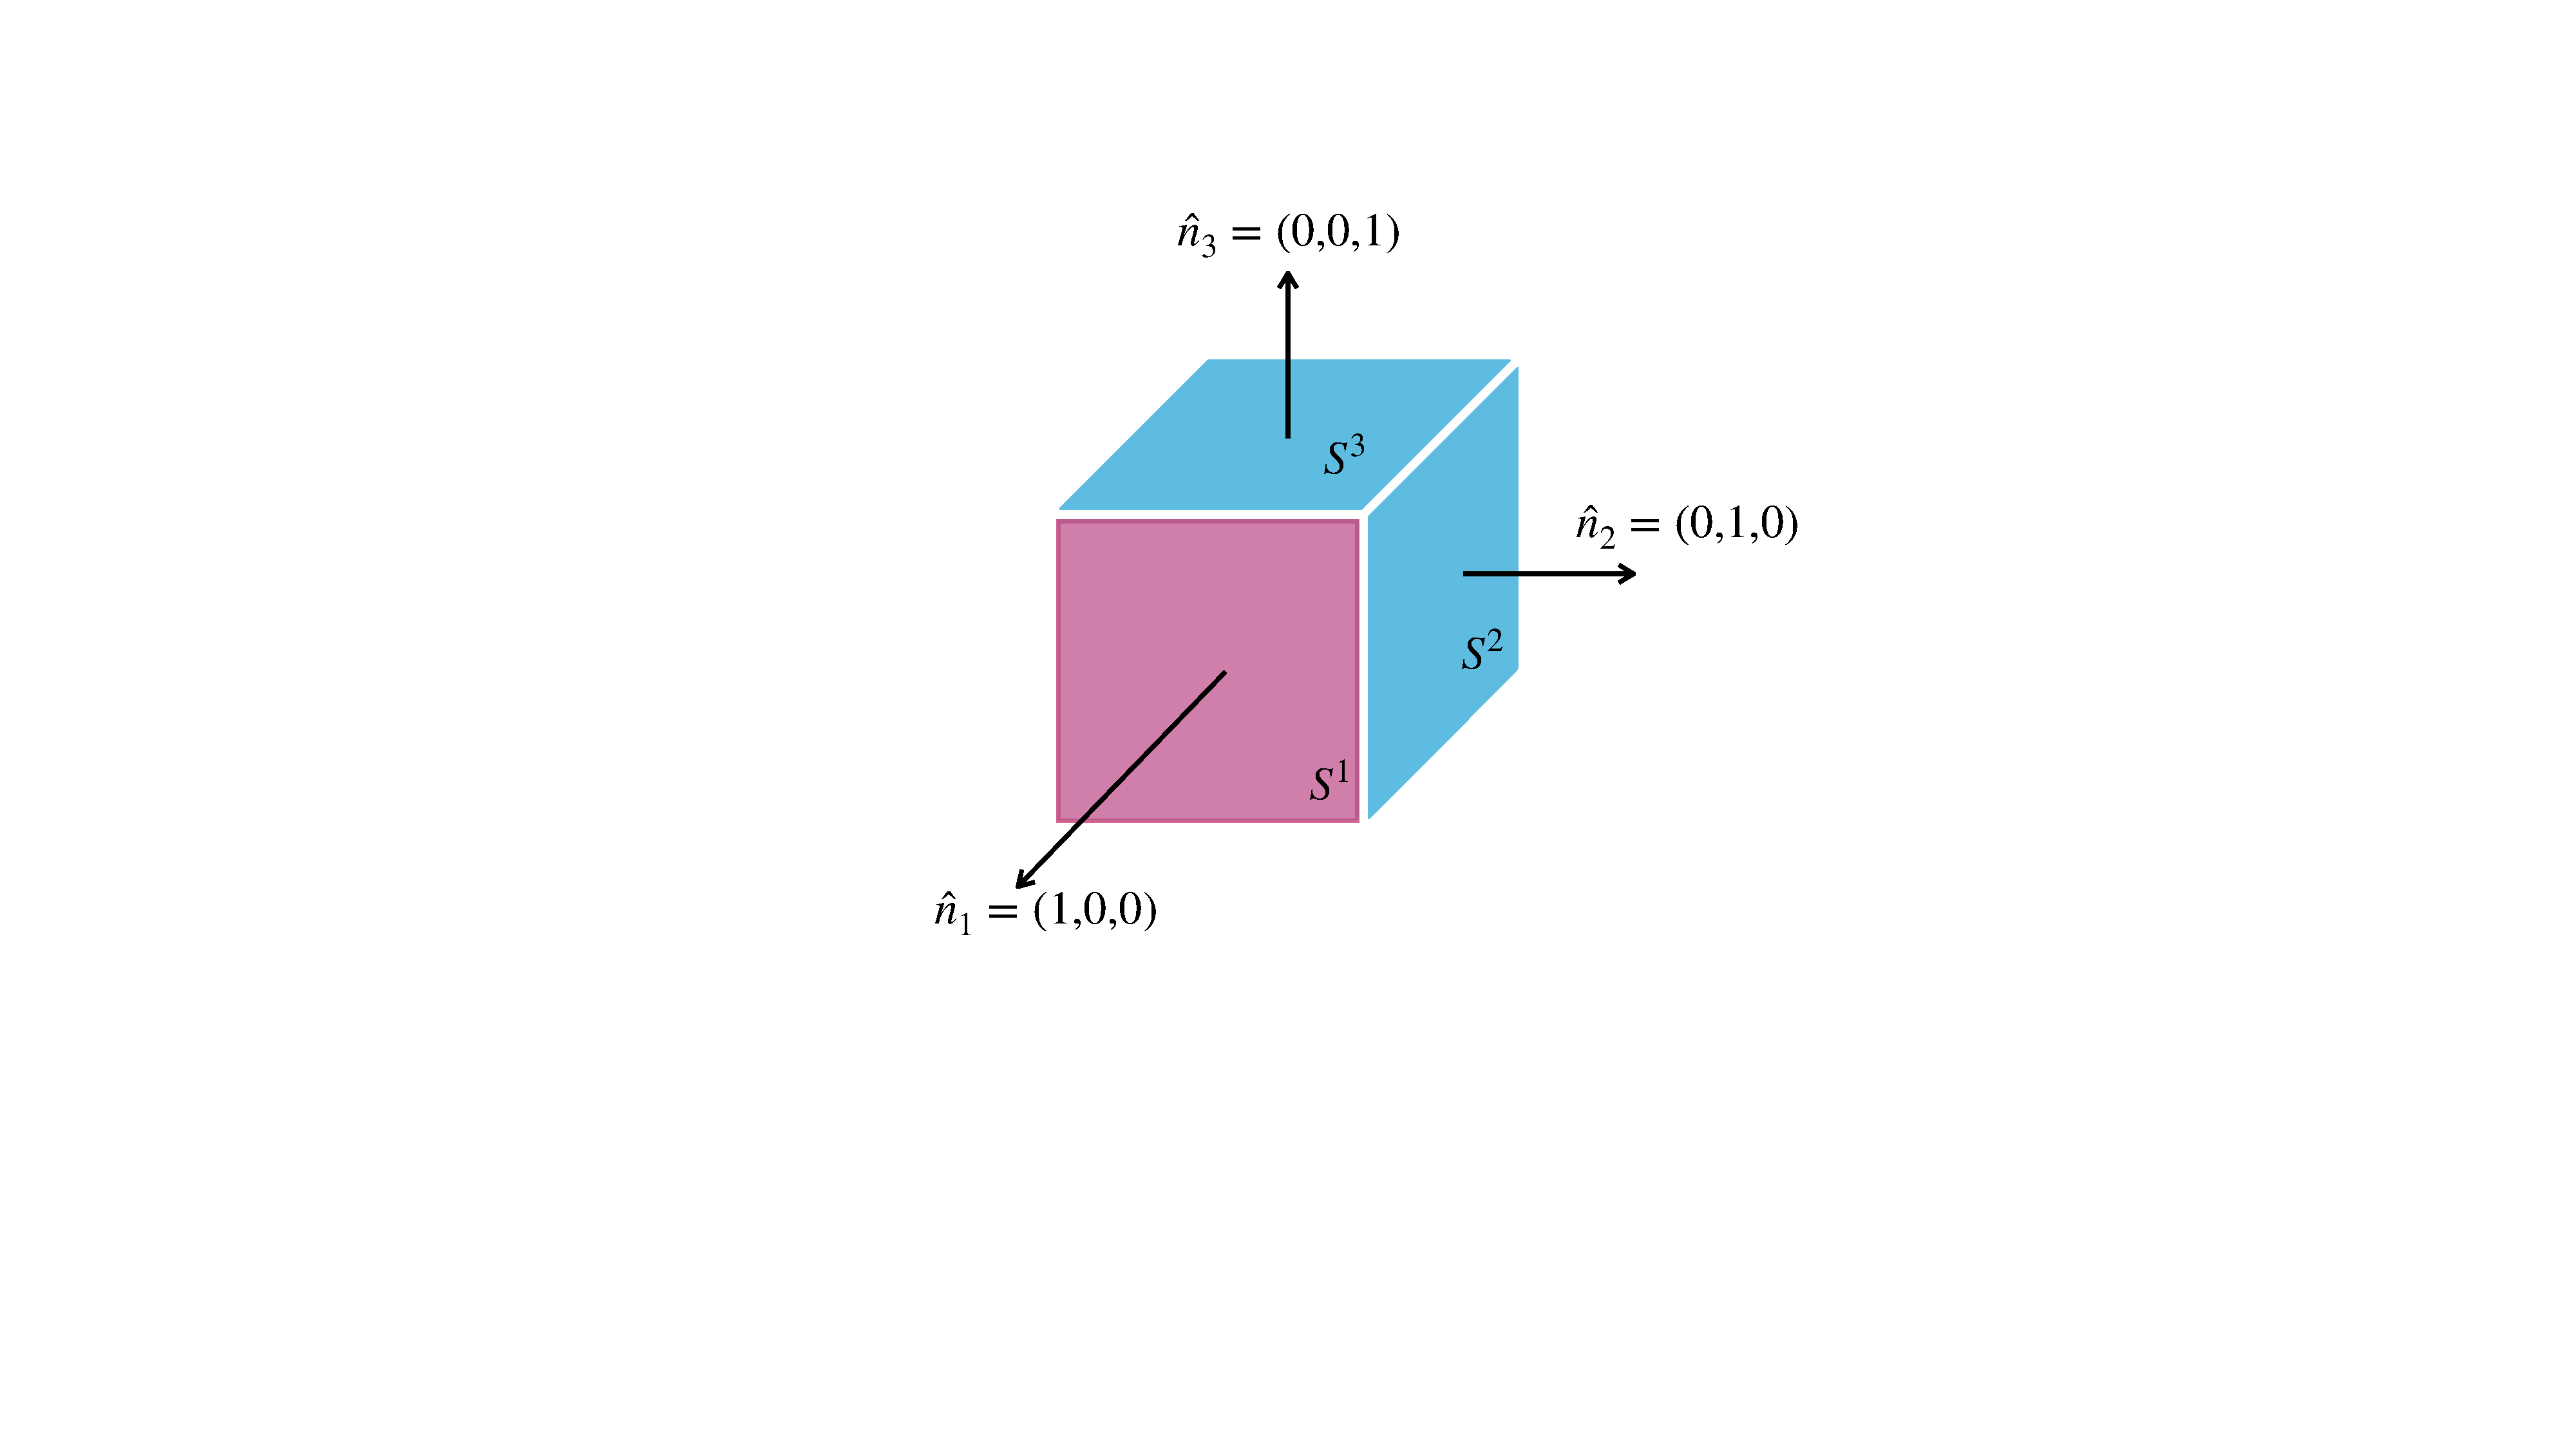
\includegraphics[scale=0.3]{./figures/fig_rho_bg_on_S1.pdf}
	\caption{Example cube to describe the buoyancy force computation. The pink area is the $S^1$ integral domain.}
	\label{fig_rho_bg_on_S1}
\end{center}
\end{figure}
Since the background density $\rho_{bg}$ is a function of $z$, we can intuitively see that the value (\ref{eq_buoyancy_S1_2}) and the one with the normal $\hat{n}_6 = -\hat{n}_1 = (-1,0,0)$ has the same magnitude but in the opposite direction, and thus, we have $\mathcal{L}_6 = -\mathcal{L}_1$. 
This implies the following,
\begin{equation}
	\sum_{i=1,2,5,6}
	 R_a^3 \int_{S^i} 
	 \mathcal{P}_{bg}(z) 
	 \bar{\bar{I \ }}  \cdot
	\hat{n}_i \ \textrm{d}S^i (\vec{x})
	 = 0
\label{eq_buoyancy_zero_oneCube}
\end{equation}
for the one cube case of discretized buoyancy equation (\ref{eq_buoyancy_discrete2}).
\par
The integrals on $S^3$ and $S^4$ are slightly different since the square faces are perpendicular to the $z-$axis. On the face $S^3$, which has normal $\hat{n}_3 = (0,0,1)$, we get
\begin{equation}
	R_a^3
\rho_0\int_{-1}^{1} \int_{-1}^{1}
  	\left( 
  	 z - \frac{\gamma}{2}{z}^2 
 	\right)g  \bar{\bar{I \ }}  \cdot
 	\hat{n}_3 \ 
	\textrm{d}x  \textrm{d}y 
	= 4 R_a^3 \rho_0 \left( z_T - \frac{\gamma}{2} {z_T}^{2} \right) g \hat{n}_3,
	\label{eq_F_by_S3}
\end{equation} 
where $z_T$ is the constant $z-$level value on the face $S^3$. The integral value on the face $S^4$ would be the same as (\ref{eq_F_by_S3}), having $\hat{n}_4 = (0,0,-1)$ instead of $\hat{n}_3$. We then can have a more explicit expression for the discretized buoyancy equation (\ref{eq_buoyancy_discrete2}),
\begin{align}
	& \sum_{i=1}^{6} R_a^3
	 \int_{S^i}
	 \mathcal{P}_{bg}(z) 
	  g \bar{\bar{I \ }}  \cdot
	\hat{n}_i \ \textrm{d}S^i (\vec{x})
	\nonumber 
	\\
	& = 4 R_a^3 \rho_0 \left( z_T - \frac{\gamma}{2} {z_T}^{2}  \right) g \hat{n}_3
	+ 4R_a^3 \rho_0 \left( z_B - \frac{\gamma}{2} {z_B}^{2}  \right) g \hat{n}_4,
\label{eq_buoyancy_discrete_eval2}
\end{align}
where $z_B$ is the constant $z-$value on the surface $S^4$ (bottom face). By substituting the normals $\hat{n}_3$ and $\hat{n}_4$, we can simplify the right-hand side of equation (\ref{eq_buoyancy_discrete_eval2}), knowing that $z_T - z_B = 2$, equation (\ref{eq_buoyancy_discrete_eval2}) becomes 
\begin{equation}
	\sum_{i=1}^{6} R_a^3
	\int_{S^i} 
	\mathcal{P}_{bg}(z) 
	g \bar{\bar{I \ }}  \cdot
   \hat{n}_i \ \textrm{d}S^i (\vec{x})
= 8 R_a^3 \rho_0 \left( 1 - \gamma z_{c_n} \right) g, 
\label{eq_buoyancy_z_eval2}
\end{equation}
where we define the $z-$component of the center of the $n-$th cube forming an aggregate, $z_{c_n}$ ($ n = 1, 2, \cdots, NC$).
We thus have shown that the only information we need to keep track of is the location of the center of each cube that forms an aggregate.
%
 \subsection{Linear system for velocity and stress on aggregates}
As mentioned in section~\ref{sec:force_balance}, we do not prescribe the settling velocity of an aggregate, and it becomes one of our unknowns.
We thus need to solve for 1) translational velocity ($\vec{U}_a$), 2) rotational velocity ($\vec{\Omega}$), and 3) stress vector ($\vec{f}_k$) on each square face $k$.
% To do so, we build a linear system using equations (\ref{eq_Fo}), (\ref{eq_Qo}). 
To do so, for any point $\vec{y}$ on the surface of the aggregate, we consider the surface velocity equations (\ref{eq_vel_all_onS_nonD}) with the solid body motion, (\ref{eq_solidbody}), 
 \begin{align}
	\vec{U}_a + \vec{\Omega} \times (\vec{y} - \vec{x}_{cm})
+ \frac{1}{8 \pi} \int_{S}  
		  \vec{f}(\vec{x}) 
		  \cdot \bar{\bar{G  }} (\vec{x},\vec{y}) 
		  \ \textrm{d}S(\vec{x})
		  \nonumber \\
=  -\frac{ \alpha C_{max}}{8\pi } \frac{\rho_0}{(\rho_s - \rho_0)(1-\phi)} 
\int_{V} C\left(\vec{x},  t \right) \hat{k} \cdot 
\bar{\bar{G}}(\vec{x}, \vec{y} ) 
\ \text{d}V(\vec{x}),
 \label{eq_slp_lin_eq}
 \end{align}
where the volume integral value on the right-hand side is known. 
To set up the linear system accordingly, We discretize the boundary integral as described in equation (\ref{eq_discretized}), choosing $\vec{f}_k$ for $\vec{q}_k$, and $ \bar{\bar{G}}$ for $\bar{\bar{J}}$, 
\begin{equation}
	\vec{I}(\vec{x}_{sq,i})  =   \sum_{k=1}^{N_f}  \vec{f}_k   \int_{S_{k}} \bar{\bar{G}}(\vec{x},\vec{x}_{sq,i}) \ \text{d}S(\vec{x}) 
	= \sum_{k=1}^{N_f} \vec{f}_k   \ \bar{\bar{\Pi}}_{i,k}
	\approx \int_{S}  
	\vec{f}(\vec{x}) 
	\cdot \bar{\bar{G  }} (\vec{x},\vec{x}_{sq,i}) 
	\ \textrm{d}S(\vec{x}),
\end{equation}
where $\vec{x}_{sq, i}$ is the center of each square on the surface for $i = 1, \  2, \cdots, \  N_f$.
With equations (\ref{eq_Fo}), (\ref{eq_Qo}), the exact linear system of the equations we implement is as follows.
 \begin{align}
	\tiny
		%---A------------------------------------------------------------
 	\left[
 	    \begin{array}{c;{2pt/2pt}c; {2pt/2pt}c}
 			\phantom{,} & \phantom{,}& \phantom{,}
 			\\
		   \begin{bmatrix}
 				\bar{\bar{\Pi}}_{1,1} & 
 				\bar{\bar{\Pi}}_{1,2} &
 				\cdots & \bar{\bar{\Pi}}_{1,N_f}
 				\\
 				\\
 				\bar{\bar{\Pi}}_{2,1} & 
 				\bar{\bar{\Pi}}_{2,2} &
 				\cdots & \bar{\bar{\Pi}}_{2,N_f}
 				\\ 
 				\vdots &  \vdots & \ddots & \vdots
 				\\
 				\\
 				\bar{\bar{\Pi}}_{N_f,1}&
 				\bar{\bar{\Pi}}_{N_f,2} &
 				 \cdots & \bar{\bar{\Pi}}_{N_f,N_f}
 		\end{bmatrix}
 			 & 
 			 \begin{bmatrix}
 				 \bar{\bar{I \ }}
 				 \\
 				 \vdots
 				 \\
 				 \\
 				  \bar{\bar{I \ }}
 			\end{bmatrix}
 			  & -
    			 \begin{bmatrix}
    				  [\vec{x}_{sq,1} - \vec{x}_{cm}]_{\times}
    				 \\
    				 \vdots
    				 \\
    				 \\
    				   [\vec{x}_{sq,N_f} - \vec{x}_{cm}]_{\times}
    			\end{bmatrix}
 			\\
 			\phantom{,} &\phantom{,} &\phantom{,}
 			\\
 			\hdashline[2pt/2pt]
 			\phantom{,} &\phantom{,} &\phantom{,}
 			\\
 			 4 \begin{bmatrix}
 				  \bar{\bar{I \ }}
 				 &
 				 \cdots
 				 &
 				  \bar{\bar{I \ }}
 			\end{bmatrix}
 			&  \bar{\bar{0}}  & \bar{\bar{0}}
 			\\
 			\phantom{,} &\phantom{,} &\phantom{,}
 			\\
 			 \hdashline[2pt/2pt]
 			 \phantom{,} &\phantom{,} &\phantom{,}
 			\\
 			 - 4 \begin{bmatrix}
 				[\vec{x}_{sq,1} - \vec{x}_{cm}]_{\times}
 				 &
 				 \cdots
 				 &
 				  [\vec{x}_{sq,N_f} - \vec{x}_{cm}]_{\times}
 			\end{bmatrix}
 			& \bar{\bar{0}}  &  \bar{\bar{0}}
  	 	\\
 			\phantom{,} & \phantom{,}& \phantom{,}
 	    \end{array}
 	\right]
 	%---x------------------------------------------------------------
 	\left[
 	\begin{array}{c}
 		\vec{f}_1
 		\\ \\
 		\vdots \\
 		\\
 		\vec{f}_{N_f}
 		 \\ \\  \hdashline[2pt/2pt]
 		\\
 		 \vec{U}_a
 	  	\\
 	 	\\
 	 	\hdashline[2pt/2pt]
 	 	\\
 	 	\vec{\Omega}
 	\end{array}
 	\right]
 		%---b------------------------------------------------------------
 	=
 	\left[
 	\begin{array}{c}
 		{\vec{\mathcal{F}}}^1  \\ \\
 		\vdots \\
 		\\
 		{\vec{\mathcal{F}}}^{N_f} \\ \\  \hdashline[2pt/2pt]
 		\\
 		 \vec{F}_o
 	  	\\
 	 	\\
 	 	\hdashline[2pt/2pt]
 	 	\\
 	 	\vec{Q}_o
 	\end{array}
 	\right].
 \label{eq_slp_linear_system}
 \end{align}
 Since we consider three-dimensional space, the size of the identity matrix $\bar{\bar{I}}$ is $(3 \times 3)$. The matrix $[\vec{y}]_{\times}$ represents the cross product operator defined by,
 \begin{equation}
 	[\vec{y}]_{\times} = \begin{bmatrix}
 	0 & -y_3  & y_2 \\ 
 	 y_3 & 0  & -y_1\\ 
 	- y_2 & y_1  & 0
 	\end{bmatrix},
 	\label{eq_cross_2}
 \end{equation}
 where $\vec{y} = (y_1, y_2, y_3).$
We use this operator for the rotation term, 
 \[
  [\vec{x} - \vec{x}_{cm}]_{\times}  \vec{\Omega}
   = (\vec{x} - \vec{x}_{cm}) \times \vec{\Omega}
  = - \vec{\Omega} \times  (\vec{x} - \vec{x}_{cm}),
  \]
in the total torque equation.
In addition, the top part of the right-hand side of the equation (\ref{eq_slp_lin_eq}) is the discretization of the volume integral,
\begin{equation}
	{\vec{\mathcal{F}}} (\vec{x}_{sq,i}) = 
	-\frac{ \alpha C_{max}}{8\pi } \frac{\rho_0}{(\rho_s - \rho_0)(1-\phi)} 
   \sum_{j= 1}^{Ns}  C \left(\vec{x}_{sq,i},  t \right) \hat{k} \cdot
   \bar{\bar{G \ }}(\vec{x}_{sq, i}, \vec{x}_{j} ),
\label{eq_volume_rhs}
\end{equation}
   where $N_s$ is the total number of grid or source points in the fluid domain. We discuss more details of the volume integral computation in the next section. 
%   ~\ref{section_volume_int}.
  One can find factor 4 multiplied by the second and third blocks on the right-hand side of the system (\ref{eq_slp_linear_system}). 
 Since we set the side length of a cube as 2, factor 4 represents the area of a square face, which is the integral domain of the total force and torque equations. 
 \par
 Once we solve the linear system and obtain the unknowns, we use equation (\ref{eq_vel_all_onS_nonD}) to calculate the velocity field at all points in the fluid domain. We want to point out that the fluid velocity computation, especially including the volume integral (\ref{eq_volume_rhs}), is a very numerically expensive calculation. To accelerate it, we apply the fast multipole method (FMM) to our simulations. In the following section, we explain how we use the FMM. 
 %
 %
 %----FMM--------------------------------------------------------------------------
\subsection{Fast Multipole Method (FMM)}
\label{subsec:FMM}
Knowing that we simulate our problem in a three-dimensional fluid domain, it is necessary to implement an efficient and fast method for each part of the code while we keep the stability and desired accuracy. 
The FMM is a numerical scheme for rapid computation of $N$-body problems governed by a Green's function using a multipole expansion. It was first introduced by Greengard and Rokhlin~\cite{greengard_fast_1987}. Since then, the researchers at Flatiron Institute - Simons Foundation,  including the original authors of the FMM, have developed the methods and shared the source code.~\cite{cheng_fast_1999,greengard_new_1997,greengard_new_2002} We choose to use their library, called \href{https://github.com/flatironinstitute/FMM3D}{{\color{blue}FMM3D}}. It provides the code of the $N-$body interactions governed by Laplace and Helmholtz equations in three-dimensions.
For our problem, we can modify the Laplace kernel, as shown in~\cite{tornberg_fast_2008}, to compute the integrals of the Stokeslet (\ref{eq_stokeslet}).
The definition of the Laplace FMM in the FMM3D library is the following:
\begin{definition} (\textit{Laplace FMM})
	\label{eq_def_FMM}
	Let $c^n \in \mathbb{R}$ denote a collection of charge strengths and $\vec{v}^n \in \mathbb{R}^3$ denote a collection of dipole strengths for $n = 1,2, \cdots, N$.
	The Laplace FMM computes the potential $u(\vec{y}^m) \in \mathbb{R}^3$ given by
\begin{equation}
	u(\vec{y}^m) = \sum_{n = 1}^{N} 
		\Biggl[
		\frac{c^n}{\|\vec{x}^n - \vec{y}^m \|}
			- \vec{v}^n \cdot \nabla_{\vec{y}} 
			 \frac{1}{\|\vec{x}^n - \vec{y}^m \|}
		\Biggr],
\label{eq_fmm3d_package}
\end{equation}
	at the \textit{source} ($\vec{x}^n$) and \textit{target} locations ($\vec{y}^m$). 
	% Here, the denominator $\|x_i^n - y_j^m \| = \|\vec{x}^n - \vec{y}^m \|$.
	When $\vec{y}^m = \vec{x}^n$, the term corresponding to $\vec{x}^n$
	is dropped from the sum.
\end{definition}
\noindent
Note that we use the letters $m$ and $n$ to index the targets and sources, respectively. For our problem, the points where we want to obtain velocity would be the targets; all points in the integral domain are sources.
In addition to the target and source points, we can input the constant $c^n$ and vector $\vec{v}^{n}$. One needs to be careful with these terms; both values could depend on the sources but are independent of the targets. 
\subsubsection{Volume integral of the Stokeslet}
We first investigate how to incorporate the volume integral (\ref{eq_volume_rhs}) (without the prefactor) in the form of (\ref{eq_fmm3d_package}). For a fixed $j$, we can rewrite the equation using the index notation ($i, j = 1,2,3$), 
\begin{equation}
	\tilde{V}(y_j^m)
	\equiv
	 d\sum_{n = 1}^{Ns} \sum_{i = 1}^{3}
	 C(x^n_i,  t)k_iG_{ij}(x_i^n,y_j^m),
	\label{eq_Vn}
\end{equation}
where $\vec{y}^m = (y_1^m, \ y_2^m, \ y_3^m)$ is the target point, $\vec{x}^n = (x_1^n, \ x_2^n, \ x_3^n)$ are the source or grid points in the fluid domain $V$, and $d$ is a constant from a quadrature method.
The Stokeslet can be expressed in terms of the Laplace kernel, $\Phi(\vec{x},\vec{y}) = 1/{\| \vec{x} - \vec{y} \|}$ as,
\begin{equation}
	G_{ij}(\vec{x}^n, \vec{y}^m)
	 =  \delta_{ij} \Phi \left(  x_i^n - y_j^m\right)
	 - \left( x_i^n - y_j^m \right)
	 \frac{\partial}{\partial  x_j}
	\Phi \left(  x_i^n - y_j^m\right)
	\label{eq_Gij}
\end{equation}
% Then the inner summation of equation (\ref{eq_Vn}) becomes
% \begin{align*}
%  \sum_{i = 1}^{3}
%  C(x^n_i,  t)\hat{k} G_{ij}(x_i^n,\vec{y}^m)
%  	=  \sum_{i = 1}^{3} C(x^n_i,  t)\hat{k}
% 	\left(
% 	\frac{\delta_{ij}}{\|x_i^n - y_j^m \|}
% 	- \left( x_i^n - y_i^m \right)
% 	 \frac{\partial}{\partial x_j}
% 	\frac{1}{\|x_i^n - y_j^m \|}
% 	\right)
% \end{align*}
By substituting the Stokeslet (\ref{eq_Gij}) into the discretized volume integral (\ref{eq_Vn}), we then get
\begin{equation}
	\tilde{V}_j (\vec{y}^m)=
	\sum_{n=1}^{Ns}
	d
   \sum_{i = 1}^{3} C(x^n_i,  t)k_i
  	\left(
  	\frac{\delta_{ij}}{\| \vec{x}^n - \vec{y}^m \|}
  	- \left( x_i^n - y_j^m \right)
  	 \frac{\partial}{\partial x_j}
  	\frac{1}{\| \vec{x}^n - \vec{y}^m \|}
  	\right)
 \label{eq_frm_lplc_stokes}
\end{equation}
Knowing that the vector $\hat{k} = (0, \ 0, \ 1)$, only the terms where $i = 3$ survive. We thus reach the simplified sum,

\begin{align}
	\tilde{V}_j (\vec{y}^m) 
	& = \sum_{\substack{n=1 \\ n \neq m}}^{Ns} 
		d \ {C}(x_3^n, t)
		\left(
			\frac{ \delta_{3j} }{\|\vec{x}^n - \vec{y}^m \|}
			- 
			 x_3^n  
			\frac{\partial}{\partial x_j}
				\frac{1}{\|\vec{x}^n - \vec{y}^m \|}
				\right)
			\label{eq_vol_target} \\
			& +
			   y_j^m  
			\sum_{\substack{n=1 \\ n \neq m}}^{Ns} 
			d \ {C}(x_3^n, t)
			\frac{\partial}{\partial x_j}
				\frac{1}{\|x_3^n - y_j^m \|} + \mathbb{V}_p.
\label{eq_vol_source}
\end{align}
We take the singularity out of the sums since the FMM3D only evaluates an integral for points $\vec{y}^m \neq \vec{x}^n \in V$. 
At a singularity, i.e.,  $\vec{y}^m = \vec{x}^n $, we use MATLAB built-in function, \verb+integral3+, to integrate numerically by defining a small cube $\mathbb{V}_p$ around the singularity point,
\begin{equation}
	\mathbb{V}_p(\vec{y}) = 
	 \int_{{V}_p}
		C (\vec{x},t ) \hat{k} \cdot 
		\bar{\bar{G \ }} (\vec{x}, \vec{y} ) 
		\ \text{d}V(\vec{x}).
		\label{eq_vol_int_singular}
	\end{equation}
We then compute $\tilde{V}$ as in equation (\ref{eq_Vn}).
We also split the last (gradient) term having $\left( x_i^n - y_j^m \right)$ in equation (\ref{eq_frm_lplc_stokes}), and write it as two summations in equation (\ref{eq_vol_source}) to point out that these two points, $x_i^n$ and $y_j^m$, represent different arguments. The point $x_i^n$ represents all points in the volume integral domain $V$, i.e., \textit{source} and $y_j^m$ is a particular point, or \textit{target}, in which we evaluate the velocity. This is important to acknowledge since the FMM3D code treats these source and target points separately, and this is the key to accelerating the computation.
% We split the gradient term into two parts since the nature of $x_3^n$ and $y_j^m$ differs. We see that $x_3^n$ relates to the source point as the FMM3D package does. However, $y_j^m$ is the target. 
% We thus need to use the library twice to compute $\tilde{V}_j (\vec{y}^m) $.
The main advantage of using FMM is that we call this FMM code only once for multiple targets with $N_s$ number of source points. 
\par
Moreover, since our summation has a vector form, while the FMM3D package returns a scalar value, we need to run this FMM3D package three times at least for each part, (\ref{eq_vol_target}) and (\ref{eq_vol_source}). 
For more details, we break down the equations to determine what are $c^n$ and $\vec{v}^n$ would be in (\ref{eq_fmm3d_package}).
First, we consider the first term in summation (\ref{eq_vol_target}),
\begin{align}
	\sum_{\substack{n=1 \\ n \neq m}}^{Ns} 
		d \ {C}(x_3^n, t)
			\frac{ \delta_{3j} }{\|x_3^n - y_j^m \|}
	 & = \left(0,\ 0, d 	\sum_{\substack{n=1 \\ n \neq m}}^{Ns}  \frac{ {C}(x_3^n, t)}{ \|x_i^n - y_j^m \|} \right)
\label{eq_vol_part1}
\end{align}
Since ${C}(x_3^n, t)\in \mathbb{R}$ for each $n$ and a fixed time $t$, we simply choose  $c^n =  {C}(x_3^n, t)$. 
The second term in the sum (\ref{eq_vol_target}) can be computed by letting $\vec{v}^n$ in equation (\ref{eq_fmm3d_package}) be the product of the standard basis vector, $\hat{e}_j$, and the constant $x_3^n  \ {C}(x_3^n, t) $, that is
\begin{align}
	\sum_{\substack{n=1 \\ n \neq m}}^{Ns} 
		d \ {C}(x_3^n, t)
		\left(
			 x_3^n  
			\frac{\partial}{\partial x_j}
				\frac{1}{\|\vec{x}^n - \vec{y}^m\|}
				\right) = 
		d \sum_{\substack{n=1 \\ n \neq m}}^{Ns} 
			x_3^n  \ {C}(x_3^n, t) 
			      \
			\nabla_{\vec{y}} 
				\frac{1}{\|\vec{x}^n - \vec{y}^m \|}.
\label{eq_vol_part2}
\end{align}
We simply repeat the FMM3D for each component. 
\par
As we mentioned, the second summation (\ref{eq_vol_source}) is slightly different since the target point is multiplied by the gradient term that can be only related to the sources. One of the critical rules in the FMM is separating the target and source terms to compute integrals rapidly. Thus, the computation of this sum requires another three uses of the FMM package and a dot product with the target point vector.
We compute the sum in the same manner as in (\ref{eq_vol_part2})
\begin{equation}
	y_j^m  
	\sum_{\substack{n=1 \\ n \neq m}}^{Ns} 
	d \ {C}(x_3^n, t)
	\frac{\partial}{\partial x_j}
	\frac{1}{\| \vec{x}^n - \vec{y}^m \|} 
	= d y_j^m  
	\sum_{\substack{n=1 \\ n \neq m}}^{Ns}  
	{C}(x_3^n, t) \
	\nabla_{\vec{y}} 
	\frac{1}{\| \vec{x}^n - \vec{y}^m\|}
\end{equation}
as we have shown in the previous summation term with the gradient. 
%---------Homogeneous velocity computation---------------------------------------
\subsubsection{Surface integral of the Stokeslet}
To obtain the fluid velocity, we use equation (\ref{eq_vel_all_onS_nonD}) for all $\vec{y} \in V$. In this computation, the evaluation of
\begin{equation}
	u_H(\vec{y})  
	= \int_S \vec{f}(\vec{x}) \cdot \bar{\bar{G \ }}( \vec{x}, \vec{y}) \ \text{d} S(\vec{x}),
	\label{eq_uH}
\end{equation}
is quite expensive, as is that of the volume integral. 
We measured CPU time while varying the total number of fluid grid points. 
In Figure~\ref{fig_time_fmm_sum}, each line represents CPU time to compute, in seconds: 1) volume integral on the aggregate surface $S$, 2) volume integral in the fluid domain $V$, 3) solving the linear system~(\ref{eq_slp_linear_system}), 4) solving the advection-diffusion equation to update the perturbation, 5) velocity evaluation in the fluid domain, and 6) sum of all above (1 - 5).
\begin{figure}[ht]
	\begin{center}
		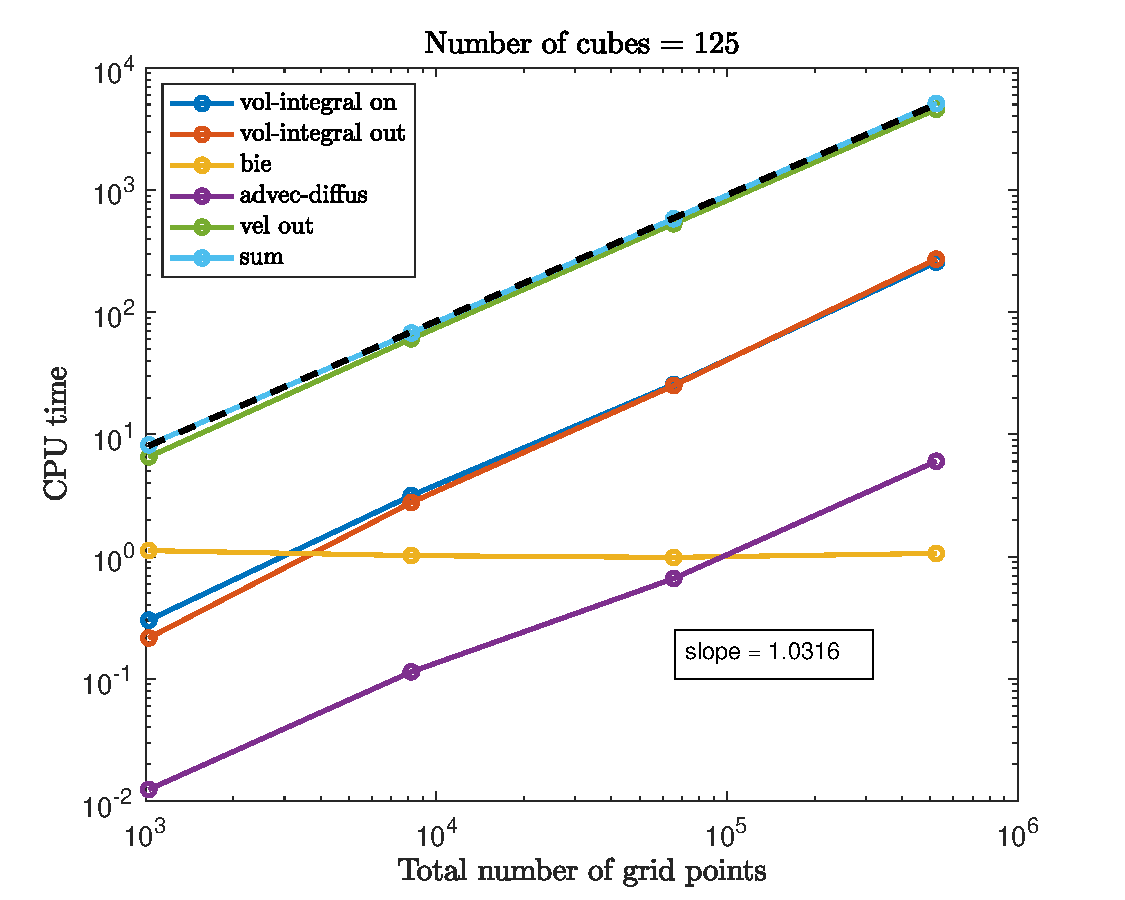
\includegraphics[scale=0.45]{./figures/fig_time_varNx5}
		% 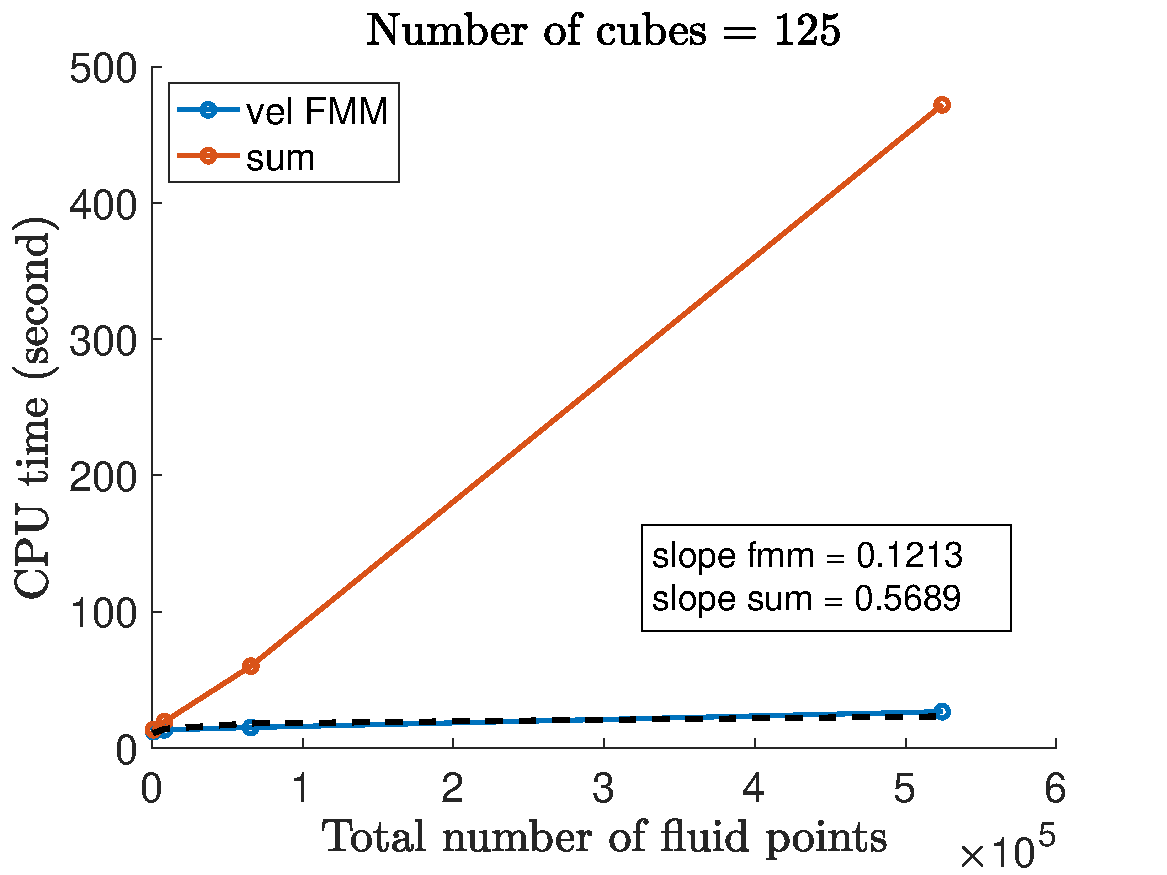
\includegraphics[scale=0.45]{./figures/fig_time_fmm_sum}
	\caption{CPU time in second with an aggregate of 125 cubes for ten time-steps.}
	\label{fig_time_fmm_sum}
\end{center}
\end{figure}
The main takeaway in this plot is that the velocity computation for all fluid points is dominant. 
We thus decided to use the FMM for this surface integral~(\ref{eq_uH}) by approximating as follows:
Here, the points $\vec{x}$ are the sources, and $\vec{y}$ are the targets. 
For the velocity inside and on the aggregate boundary, we use the rigid boundary velocity $u(\vec{x}) = \vec{U}_a + \vec{\Omega} \times \left(\vec{x} - \vec{x}_{cm} \right)$. This implies that we only use targets located outside the aggregate, and we do not expect any singularity in this computation ($\vec{x} \neq \vec{y}$). However, we may have close evaluation problems. We will discuss the size of errors in the next section. 
\par
We handle the integration of the Stokeslet in a manner similar to what was done for the volume integral. 
Using the Laplace kernel, we can re-write the surface integral (\ref{eq_uH}) as
\begin{equation}
	u_H(\vec{y}) =
	\int_S 
	\vec{f}(\vec{x}) \cdot
  	\left(
  	\frac{\bar{\bar{I \ }}}{\|\vec{x} - \vec{y}\|}
  	- \left( \vec{x} - \vec{y} \right)
  	 \nabla_{\vec{y}}
  	\frac{1}{\|\vec{x} - \vec{y}\|}
  	\right)
	  \ \text{d} S(\vec{x}).
 \label{eq_surf_laplace}
\end{equation}
We first discretize the entire aggregate surface into $N_f$ square faces located at $[cx_j^n-1, cx^n_j+1]$, where $(cx^n_1, cx^n_2)$ is the center of $n$ square face. The discretized version of the velocity equation (\ref{eq_surf_laplace}) is denoted by $H(\vec{y})$,
\begin{align}
	H(\vec{y}^m) & = u_H(\vec{y}) - E_f
	 = \sum_{n = 1}^{N_f} H^n(\vec{y}^m) 
	\nonumber \\
	& = \sum_{n = 1}^{N_f} 
	\vec{f}(\vec{x}^n) \cdot
	\int_{cx^n_2-1}^{cx^n_2+1} \int_{cx_1^n-1}^{cx_1^n+1}
  	\left(
  	\frac{\bar{\bar{I \ }}}{\|\vec{x}^n - \vec{y}^m\|}
  	- \left( \vec{x}^n - \vec{y}^m \right)
  	 \nabla_{\vec{y}^m}
  	\frac{1}{\|\vec{x}^n - \vec{y}^m\|}
  	\right)
	  \text{d} x_1  \text{d} x_2
	  ,
 \label{eq_surf_fmm_N_f}
\end{align}
where the error coming from this approximation is denoted as $E_f$. A more detailed analysis regarding $E_f$ can be found in section~\ref{sec:bie_validataion}.
 Note that the stress $\vec{f}(\vec{x}^n)$ is assumed to be constant over each square face.  One can find that we have a significant error in the cube's corners. We want to ensure that we do not introduce larger errors as we make further approximations. 

\par
Next, we need to approximate the surface integral in equation (\ref{eq_surf_fmm_N_f}) using a Riemann sum,
\begin{align}
	\tilde{H}(\vec{y}^m) 
	& = H^n(\vec{y}^m) - E_{G} 
	\nonumber \\ 
	& =
	\sum_{n = 1}^{N_f} 
	\vec{f}(\vec{x}^n) \cdot
	\sum_{s=1}^{Ns^2} d^2 
  	\left(
  	\frac{\bar{\bar{I \ }}}{\|\vec{x}_s^n - \vec{y}_s^m\|}
  	- \left( \vec{x}_s^n - \vec{y}^m \right)
  	 \nabla_{\vec{x}_s^n}
  	\frac{1}{\|\vec{x}_s^n - \vec{y}^m\|}
  	\right)
	  - E_{G},
 \label{eq_surf_fmm_N_f_n}
\end{align}
where $E_G$ is the error coming from the quadrature method. 
We use $N_s^2$ sub-squares with sizes of $d = 2/N_s$ and take the center of each sub-squares as the integration point. 
We take the same number of points, $N_s$, evenly distributed in one direction. 
In the schematic, Figure~\ref{fig_face_grid}, the red cross represents the center of the $n-$th square face, $(cx^n_1, cx^n_2)$.
\begin{figure}[h]
	\begin{center}
		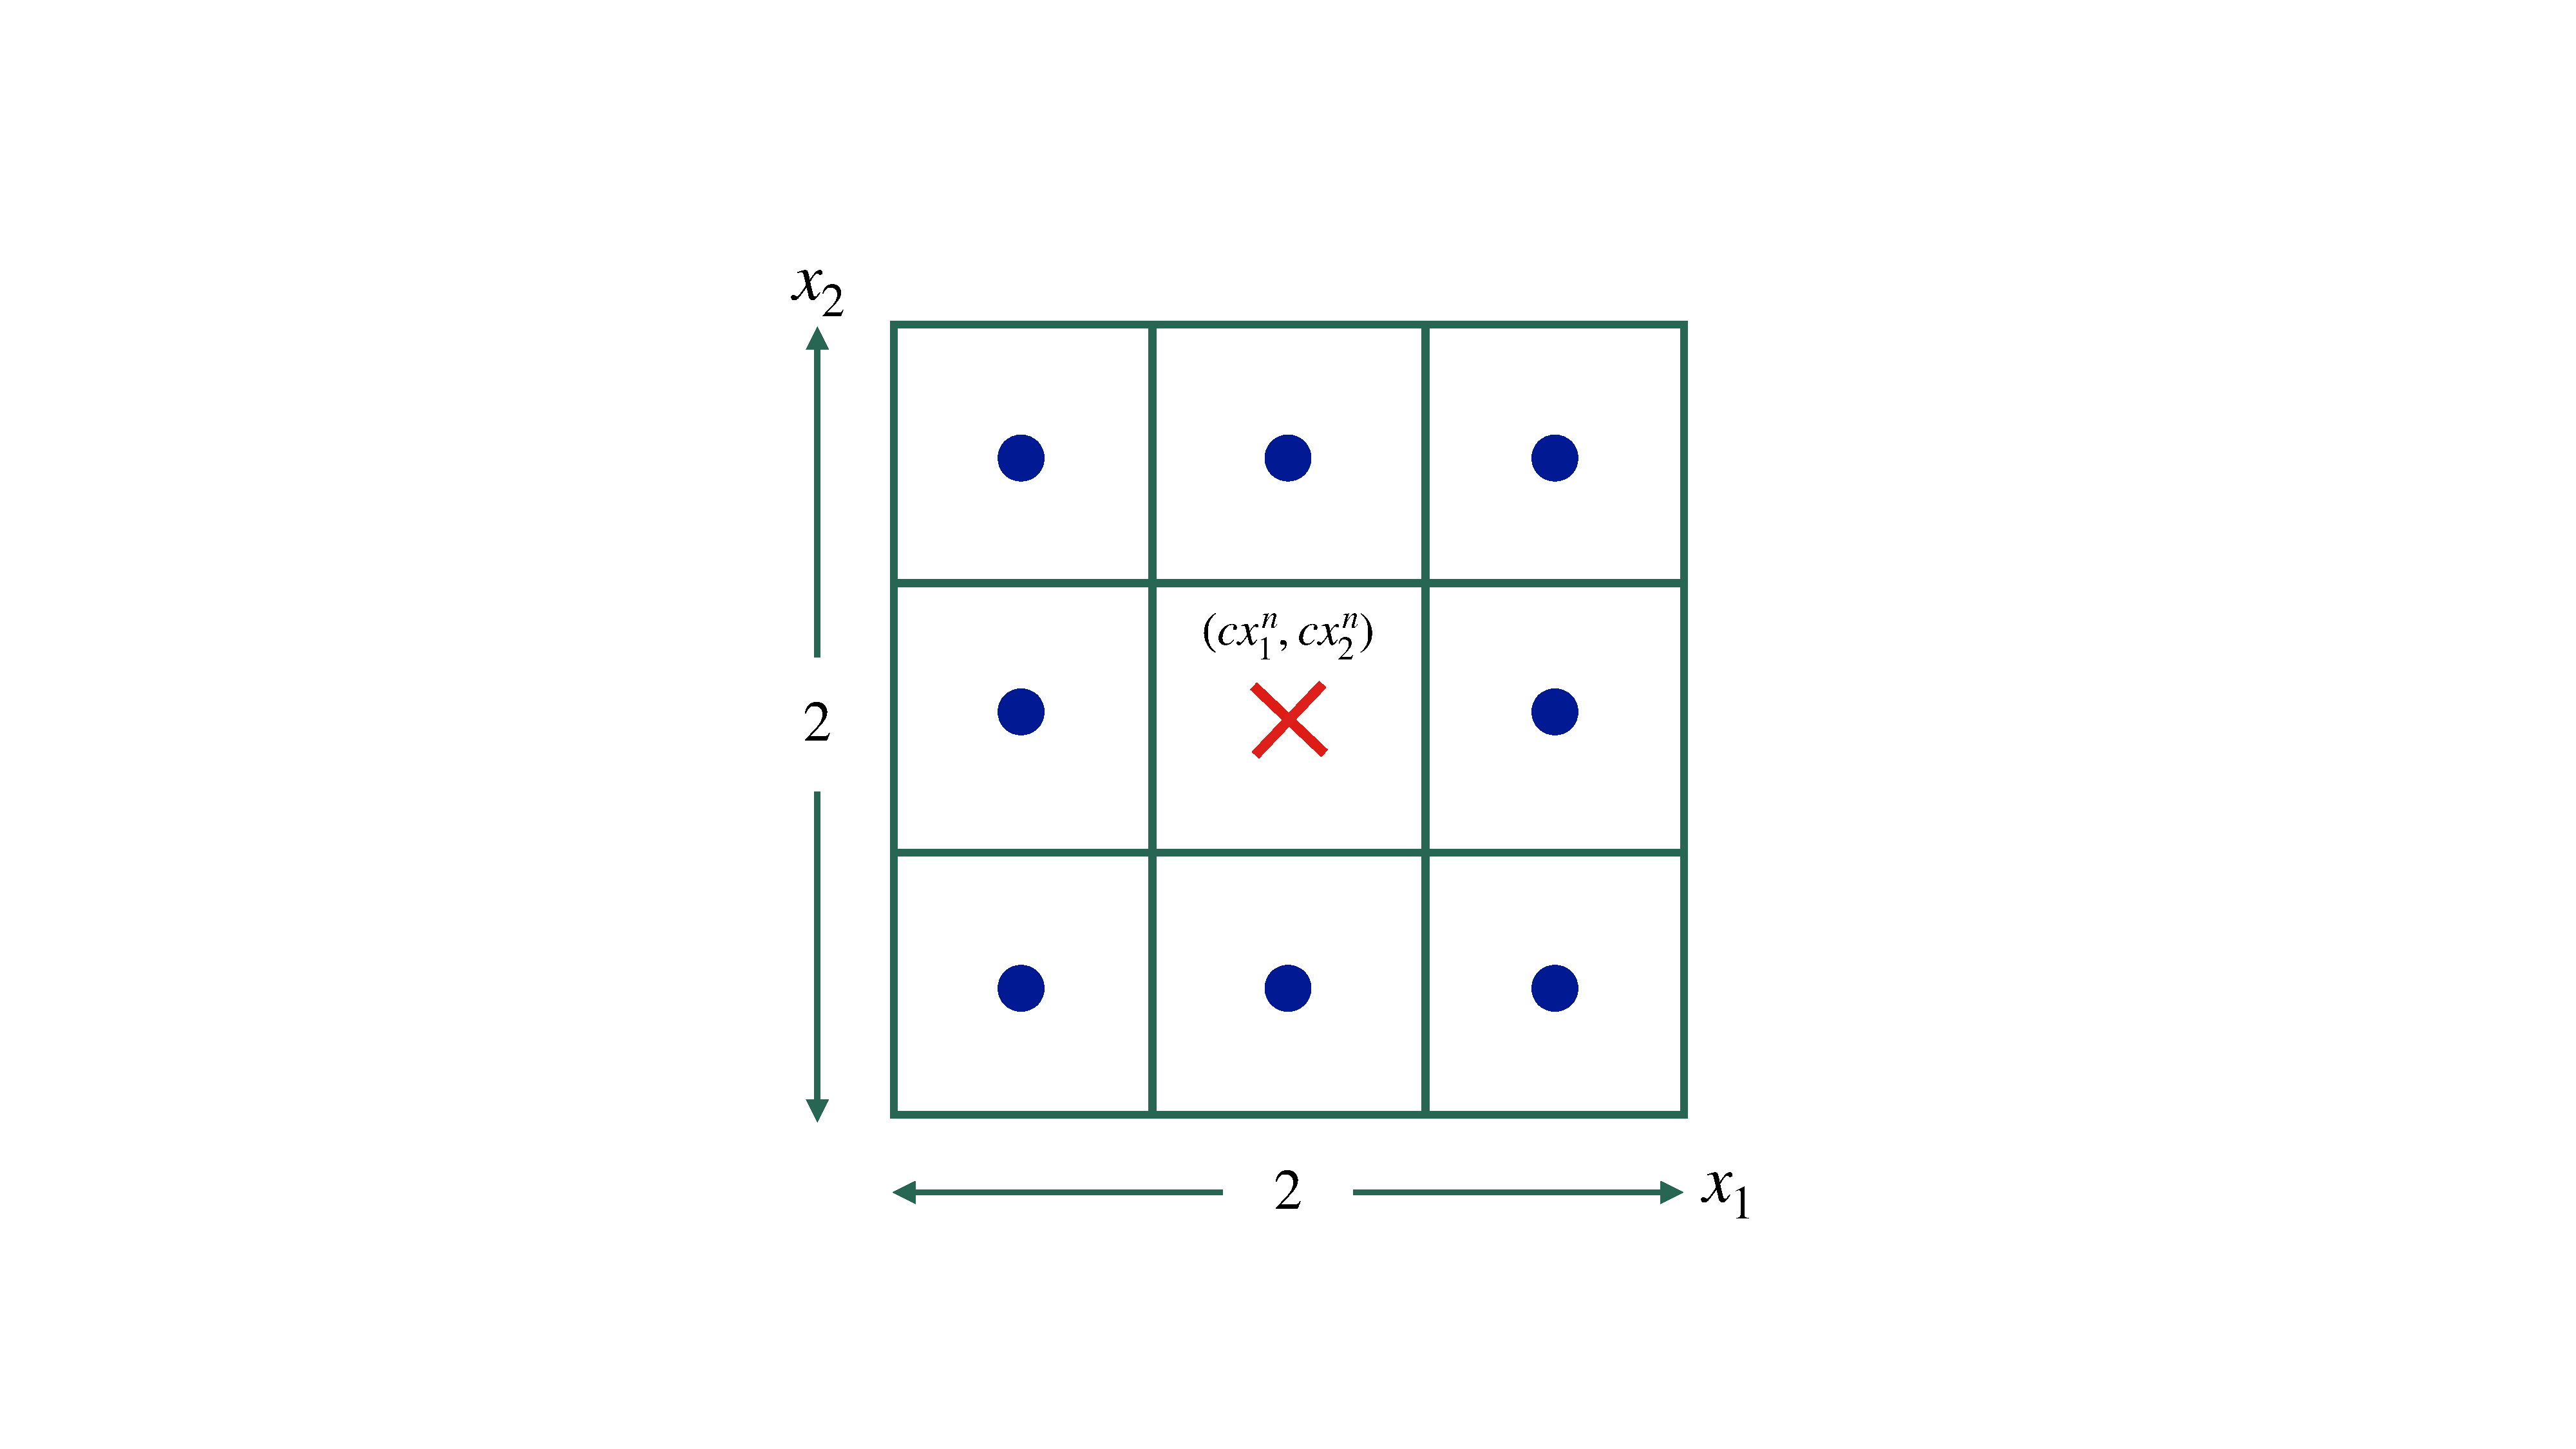
\includegraphics[scale=0.17]{./figures/fig_face_grid}
	\caption{Schematic of points we use to approximate the integral of the single-layer potential kernel over one square face.}
	\label{fig_face_grid}
\end{center}
\end{figure}
The blue dots and the red cross are the integration points.
We do not include any boundary values on one square face for simplicity.
\par
As mentioned, we hope to have a small integration error, i.e., $E_G \ll E_f$.
To measure $E_f$, we consider the settling of one cube-shaped aggregate.
We then observe the relative error of the vertical velocity on one square face, considering the translational velocity, $\vec{U}_a$, as the exact solution.
\begin{figure}[h]
	\begin{center}
		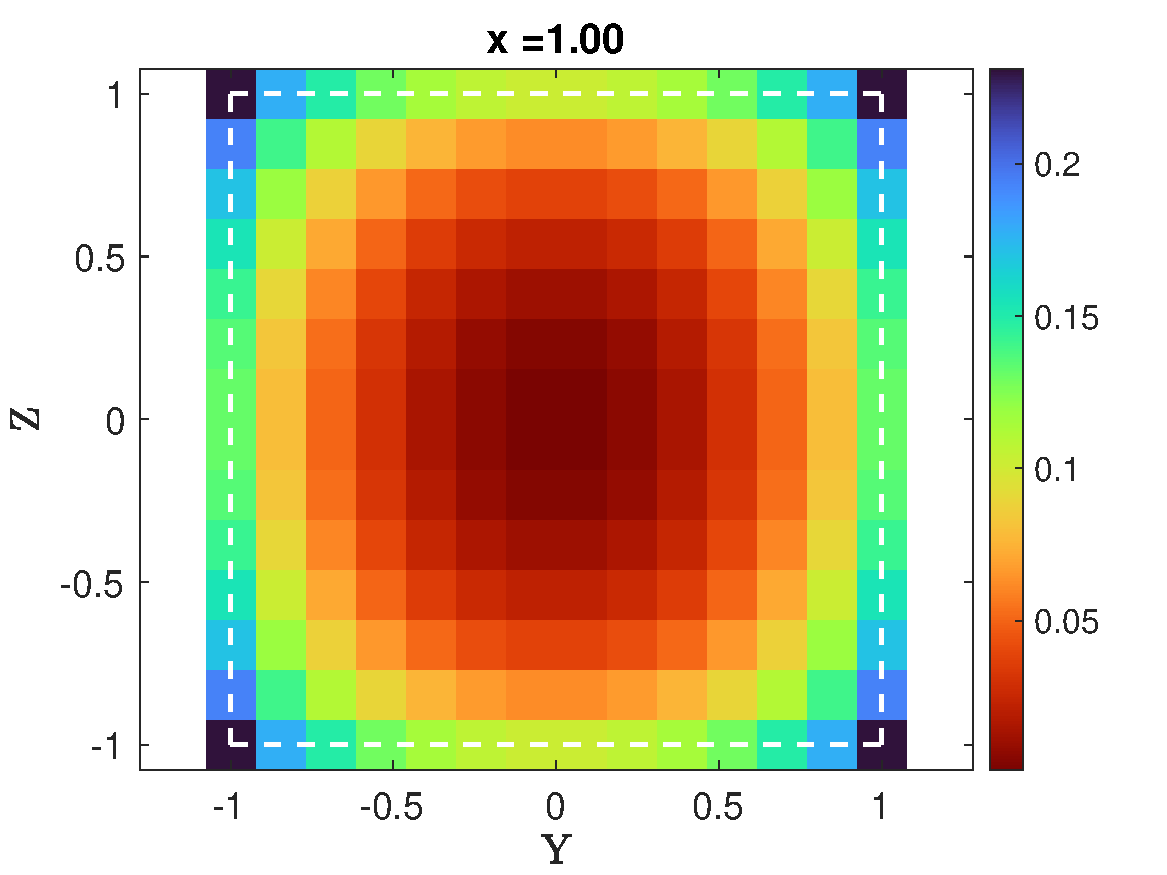
\includegraphics[scale=0.3]{./figures/fig_corner_err}
	\caption{Sample case of the relative velocity error on one face, $E_f$.}
	\label{fig_corner_err}
\end{center}
\end{figure}
In Figure~\ref{fig_corner_err}, we see the square face at $x = 1$, where the white dashed line shows the location of the square face, and the color indicates the relative error. It implies that the maximum of 23.12$\%$ error occurs at the cube corners, as we expected. We thus would like to control the quadrature error, $E_G$, by adjusting the total number of integration points, $Ns^2$.
\begin{figure}[ht]
	\begin{center}
		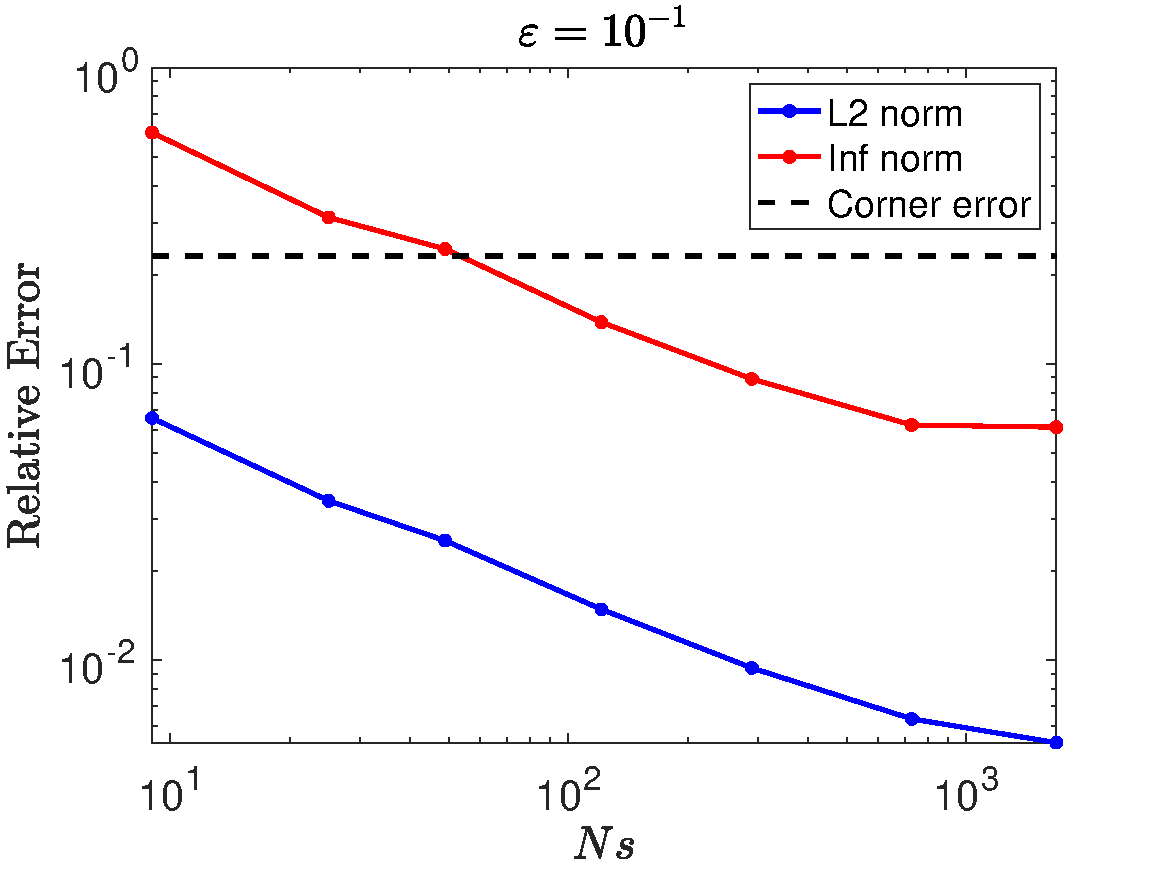
\includegraphics[scale=0.4]{./figures/fig_Ef_Eg_ep-1}
	\caption{Relative error between $U^*$ and $U^{*+}$, varying the number of integration points: $Ns = [3, 5, 7, 11, 17, 27,41]^2$ and $\varepsilon = 10^{-1}$.}
	\label{fig_Ef_EG_compare}
\end{center}
\end{figure}
\par
Two parameters affect the efficiency and accuracy of the FMM computations: 1) the number of quadrature points, $N_s^2$, and 2) the tolerance $\varepsilon$ in the FMM3D library, which determines the number of terms in the series expansion.
In Figure~\ref{fig_Ef_EG_compare}, we vary the number of integration points to choose an optimal value. 
We test a single-time simulation in the domain,  $[-5, 5] \times [-5, 5] \times [-10, 10]$,  with the one cube aggregate model. To check the responses of varying $\varepsilon$ values, we simulated the same setup with two tolerance values, $\varepsilon = 10^{-1}, \ 10^{-6}$.
From this analysis, we chose that $Ns = 9^2$ quadrature points as the error is of a size we can tolerate. We had similar results for the $\varepsilon = 10^{-6}$ case. We did not notice any difference in accuracy. We may observe this because the corner error, $E_f$, dominates our approximation and is already larger than $10 \%$. 
\begin{figure}[ht]
	\begin{center}
		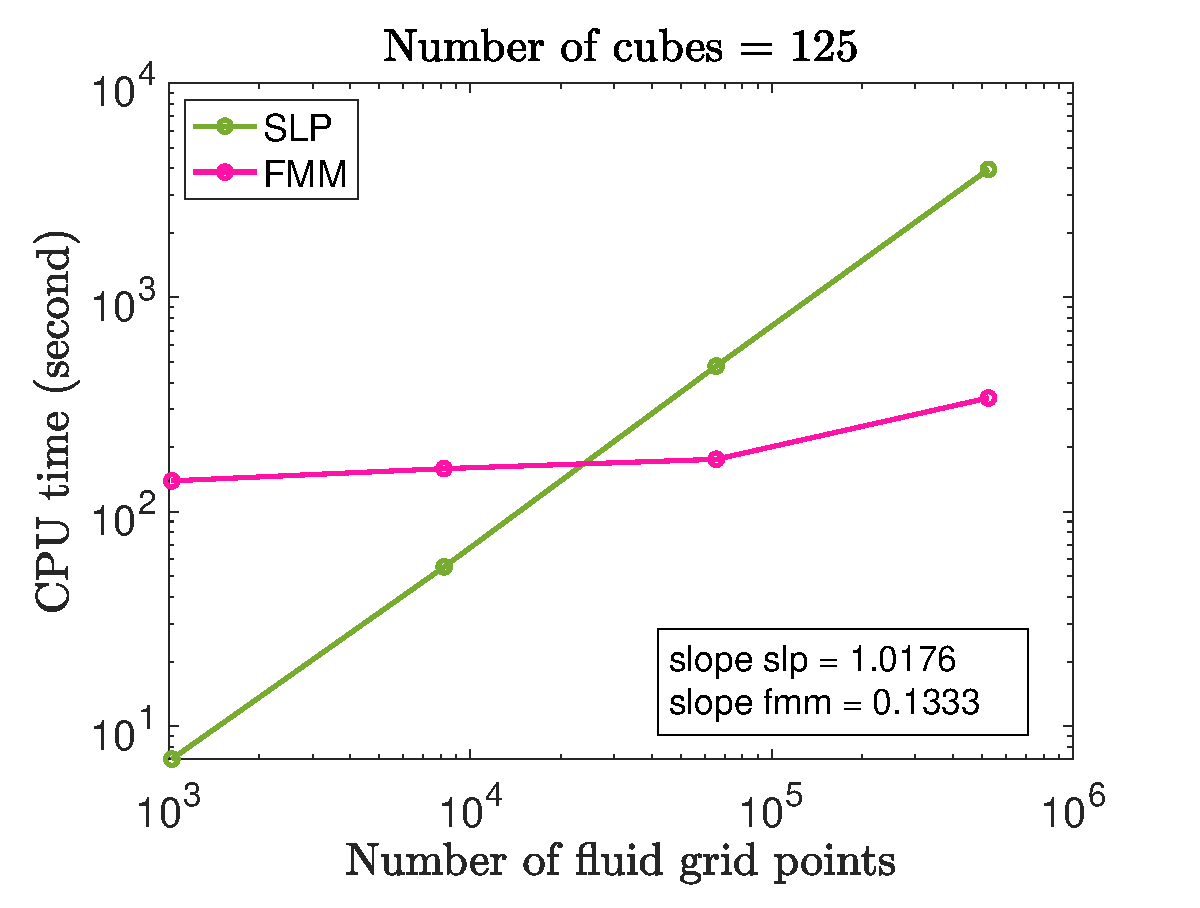
\includegraphics[scale=0.4]{./figures/fig_time_both_mm5_Nt10}
	\caption{CPU time with an aggregate made with 125 cubes for ten time steps. The green line is the velocity computation with the original single-layer potential code, and the pink line represents the approximation using the FMM3D library.}
	\label{fig_vel_mm5_t1}
\end{center}
\end{figure}
After implementing the FMM3D library into our program, we checked the compute time to compare the fluid velocity computation previously shown as the green (or dashed line) in Figure~\ref{fig_time_fmm_sum}. In Figure~\ref{fig_vel_mm5_t1}, we observe that the efficiency of the computation increases about ten times when the number of fluid grid points is about 500,00, which is in the range of what we will use to compute the fully stratified simulations.
%Rotation==============================================
\subsection{Rotation}
To have more realistic simulations, we allow our model aggregates to rotate while they settle.
In this section, we focus on the angular velocity, $\vec{\Omega} = \Delta \theta / \Delta t$, which tells us how much the aggregate rotates, $\Delta \theta$ in one time step, $\Delta t$. 
\begin{figure}[ht]
	\begin{center}
		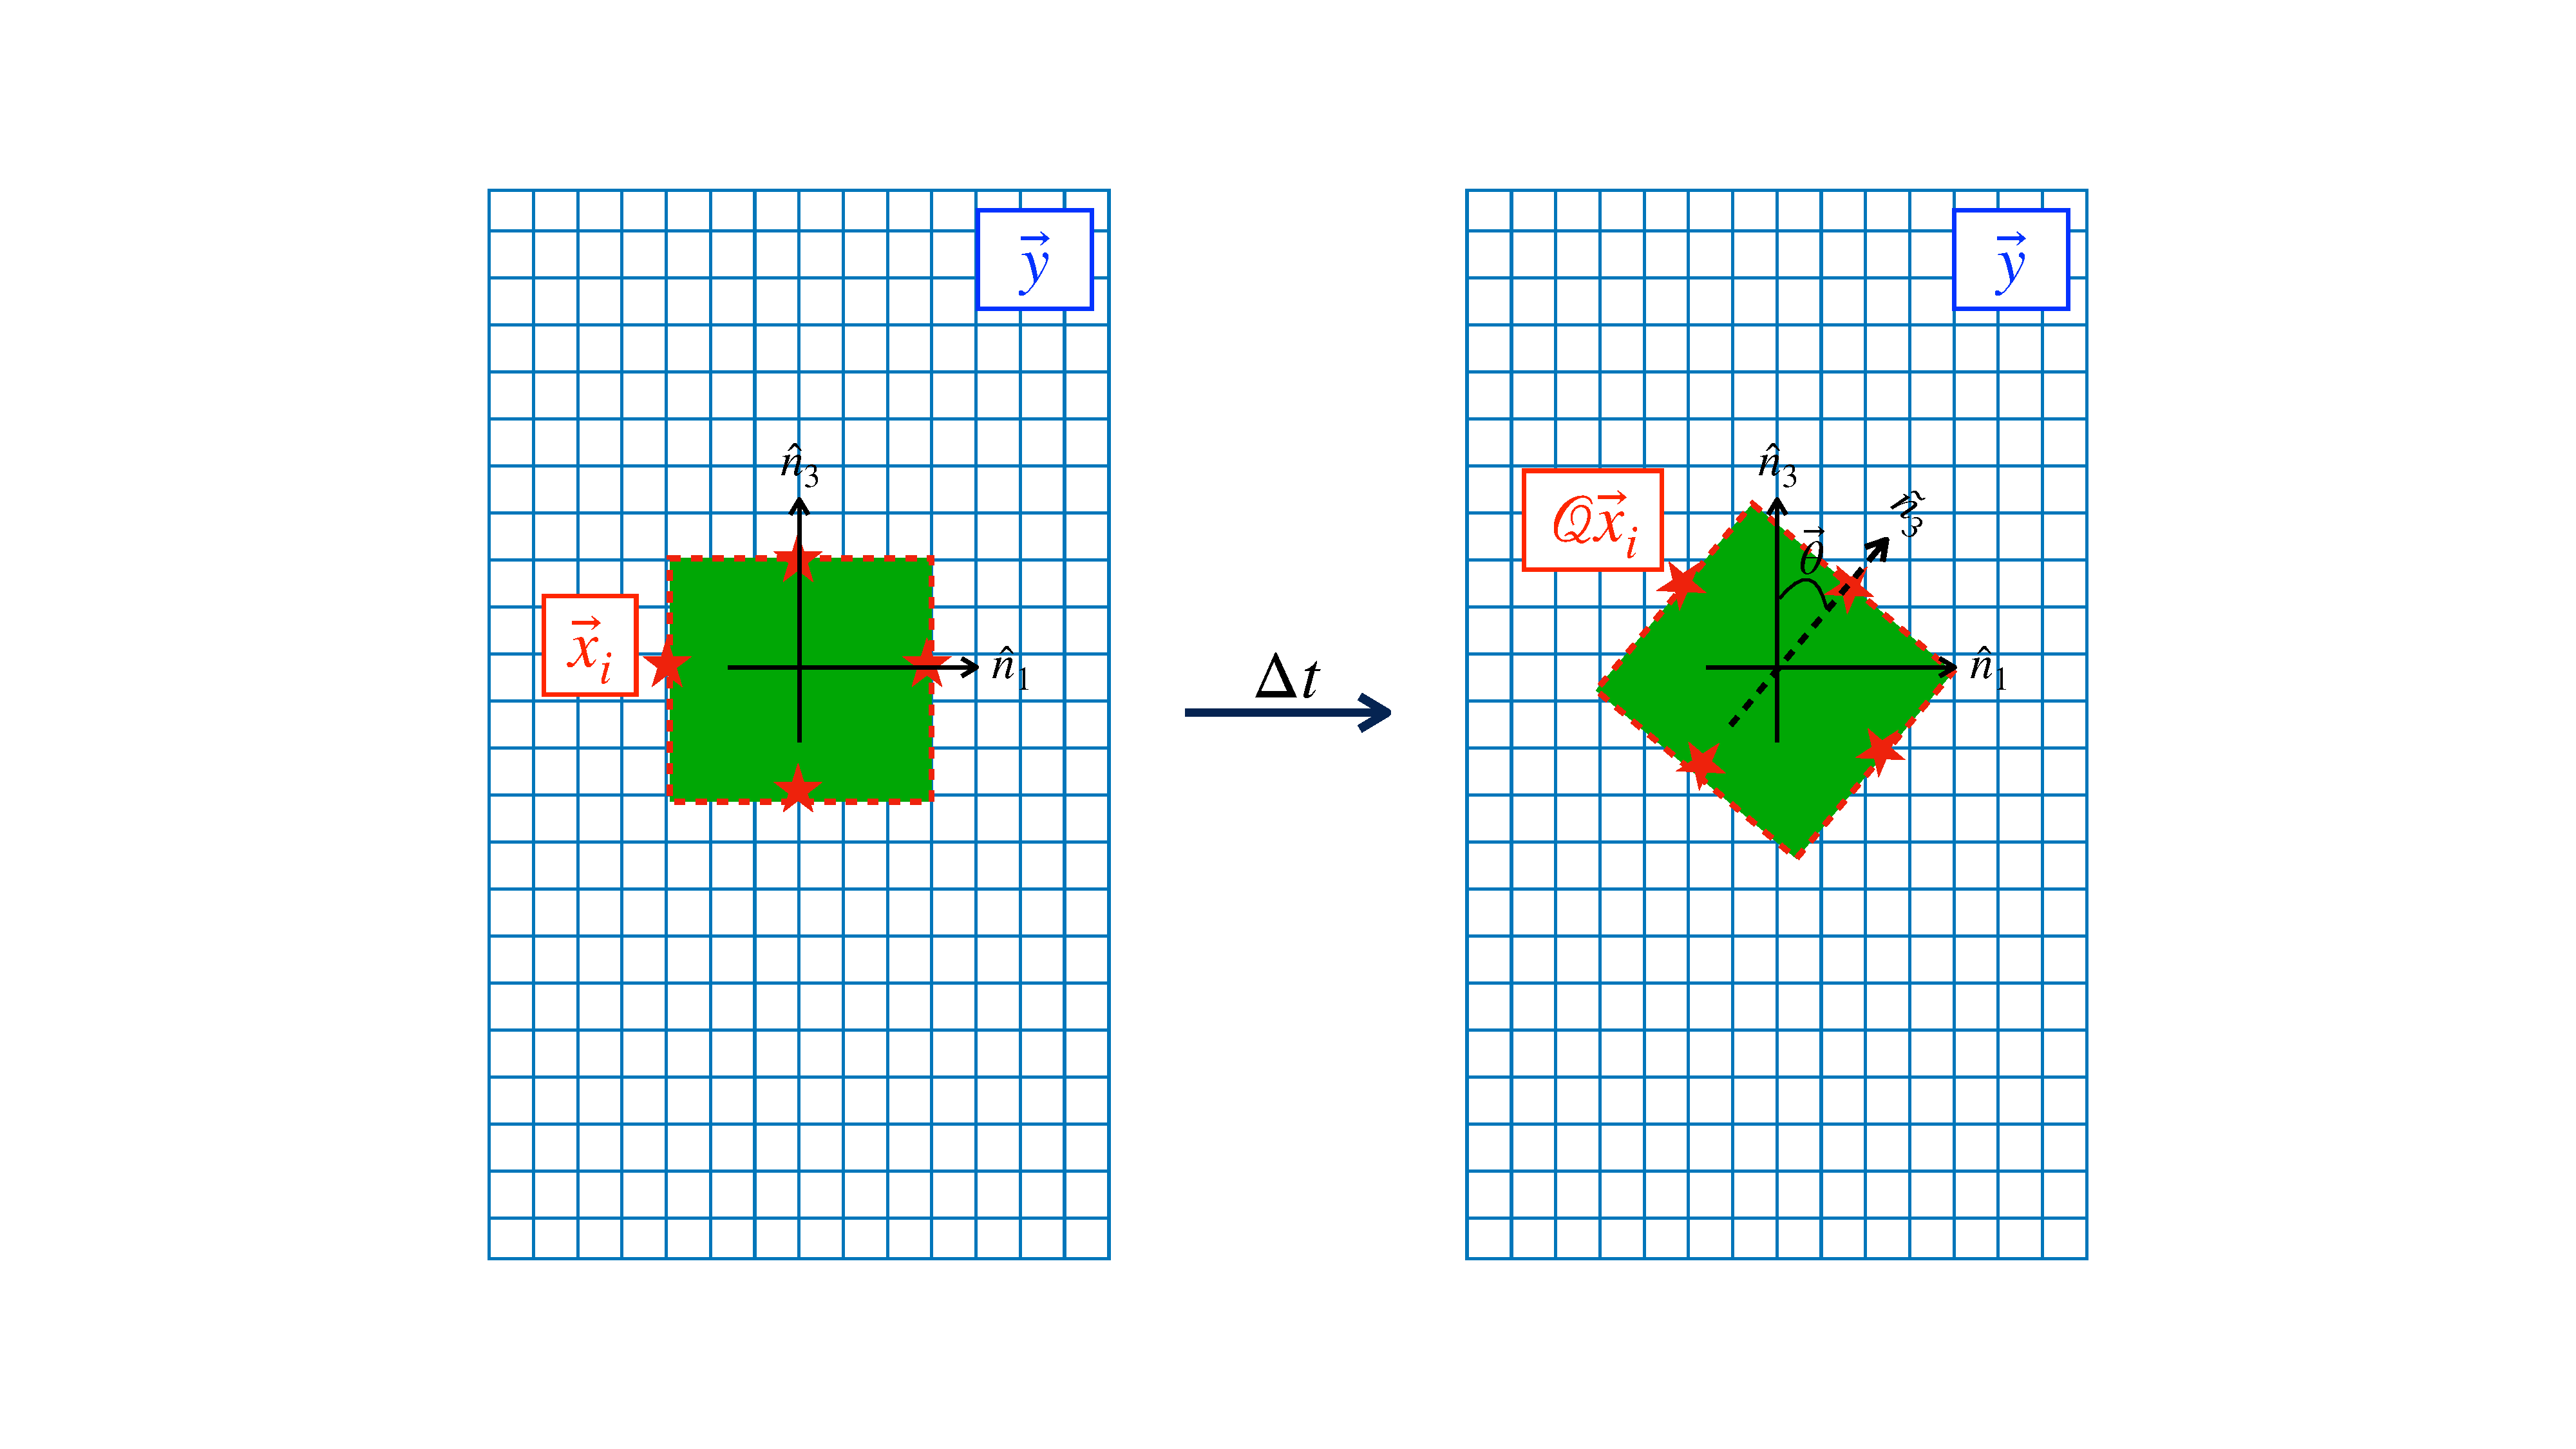
\includegraphics[scale=0.25]{./figures/fig_rotation_schematics.pdf}
	\caption{Schematics of the rotation of an aggregate. The blue grid is the fluid domain and the green rectangle represents an aggregate. Red stars show points on the aggregate.}
	\label{fig_rotation_schematics}
\end{center}
\end{figure}
This information is stored in the orientation matrix, $\mathcal{Q}(t)$. 
We can compute the position, $\vec{x}_{\mathcal{R}}(t)$ of a point on the surface of the rotated aggregated using
\[
\vec{x}_{\mathcal{R}}(t) = \mathcal{Q}(t) \vec{x}_a,
\]
where $\vec{x}_a $ is the position of a point of the aggregate surface relative to the center of mass expressed in a coordinate system that rotated with the aggregate. We note that $\vec{x}_a$ is constant in time and $\mathcal{Q}(0) = \bar{\bar{I}}$ (identity matrix) initially. After we move forward one time step, we update this orientation matrix as 
\begin{equation}
	\mathcal{Q}(t + \Delta t) = \mathcal{R} \mathcal{Q}(t),
\end{equation} 
where $\mathcal{R}$ is a rotation matrix. 
\par
We implement updates to the orientation matrix as follows~\cite{polimeno_toward_2022}.
Assume we obtain the angular velocity, $\vec{\Omega}$, from solving equation (\ref{eq_slp_linear_system}) at every time step. (Initially, it is the zero vector). With this, we can find the three-dimensional change of the angular position vector, $ \vec{\Omega} \Delta t = \left( \Delta \theta_1, \ \Delta \theta_2, \ \Delta \theta_3 \right) \equiv \Delta \vec{\theta}$.
The matrix $\mathcal{A}$ is then defined such that $\mathcal{A} \vec{x} = \Delta \theta \times \vec{x}$,
\begin{equation}
	\mathcal{A}
	=\begin{bmatrix}
	 0 & - \Delta \theta_3 & \Delta \theta_2  \\
	 \Delta \theta_3 & 0  & -\Delta \theta_1  \\
	 - \Delta \theta_2 & \Delta \theta_1 & 0  \\
	\end{bmatrix},
	\label{eq_rotation_mx}
\end{equation}
From here, we have the rotation matrix $\mathcal{R} = e^{\mathcal{A}}.$
We can compute the matrix exponential $e^{\mathcal{A}}$ using Rodrigues' formula, for antisymmetric matrices
\begin{equation}
	\mathcal{R} = 
e^{\mathcal{A}} 
 = \bar{\bar{I \ }} 
 + \frac{\sin(\phi)}{\phi} \mathcal{A}
 + \frac{1-\cos(\phi)}{\phi^2} \mathcal{A}^2,
\label{eq_R_eA}
\end{equation} 
where $\phi = \|\Delta \vec{\theta}\|_2$.
With this $\mathcal{R}$ and orientation matrix $\mathcal{Q}$, we are ready to update the fluid grid.


	
\subsubsection{Linear system in a rotated coordinate}
We first solve for the stress at the center of each square face of an aggregate, $\vec{y} = \vec{x}_i$, 
using the same formula as equation (\ref{eq_vel_all_onS_nonD}),
\begin{equation}
	\vec{u} \left(\vec{x}_i \right) 
		  = -\int_{S}  
		 \vec{f}(\vec{x}) 
		 \cdot \bar{\bar{G \ }} (\vec{x}, \vec{x}_i) 
		 \ \textrm{d}S 
		 - \frac{ \alpha C_{max}}{8\pi } \frac{\rho_0}{(\rho_s - \rho_0)(1-\phi)}
		 \int_V  C \left(\vec{x} ,t \right) \hat{k} \cdot
		 \bar{\bar{G \ }}(\vec{x}, \vec{x}_i)
		 \ \text{d}V,
		 \nonumber
\end{equation}
As we allow rotation, we can express the above equation in a rotated frame of reference using $\vec{x}_{r, i} = \mathcal{Q} \vec{x}_i, \ \vec{u}_r = \mathcal{Q} \vec{u}$, and $\vec{f}_r = \mathcal{Q} \vec{f}$,
\begin{align}
	\vec{u}_r(\vec{x}_{r, i}) =
	\mathcal{Q}
	\vec{u} \left(\mathcal{Q} \vec{x}_i \right) 
		  = & - \frac{1}{8 \pi} \int_{S}  
		 \vec{f}_r(\mathcal{Q} \vec{x}) 
		 \cdot \bar{\bar{G \ }} (\mathcal{Q} \vec{x},\mathcal{Q}\vec{x}_i) 
		 \ \textrm{d}S
		 \nonumber \\
		 & - \frac{ \alpha C_{max}}{8\pi } \frac{\rho_0}{(\rho_s - \rho_0)(1-\phi)}
		 \int_V  C \left(\vec{x} ,t \right) \hat{k} \cdot
		 \bar{\bar{G \ }}(\vec{x}, \mathcal{Q} \vec{x}_i)
		 \ \text{d}V.
	\label{eq_slp_On_rotate}
\end{align}
Since the rotation matrix $\mathcal{Q}$ is constant in space and is a rotation matrix, it is valid to say that
\[
 \bar{\bar{G \ }} (\mathcal{Q} \vec{x},\mathcal{Q}\vec{x}_i) 
	 = \bar{\bar{G}}( \vec{x}, \vec{x}_i).
\]
We now solve for unknowns, including the translational and angular velocities,
in a rotated coordinate system $\vec{x}_{r,i} $.
Note that the stress values we obtain here 
are located in the rotated positions.  
To complete the linear system to solve for stress, translational, and angular velocities, we temporarily map the fluid domain grid into the same coordinate system as the boundary integral term.
We can multiply by $\mathcal{Q}^{-1} = \mathcal{Q}^{T}$ as 
\begin{align}
	 \vec{u} \left(\mathcal{Q} \vec{x}_i \right) 
		= &
		 -\mathcal{Q}^{-1}
		 \biggl(
		 \frac{1}{8 \pi} \int_{S}  
		 \vec{f}_r(\mathcal{Q} \vec{x}) 
		 \cdot \bar{\bar{G \ }} (\mathcal{Q} \vec{x},\mathcal{Q}\vec{x}_i) 
		 \ \textrm{d}S \biggl)
		 \nonumber \\  
		 & -\mathcal{Q}^{-1}
		 \biggl(
		 \frac{ \alpha C_{max}}{8\pi } \frac{\rho_0}{(\rho_s - \rho_0)(1-\phi)}
		 \int_V  C \left(\vec{x} ,t \right) \hat{k} \cdot
		 \bar{\bar{G \ }}(\vec{x}, \mathcal{Q} \vec{x}_i)
		 \ \text{d}V
		 \biggr).
	\label{eq_slp_vol_R}
\end{align}
For the other force equations as well, we implement the following
\begin{equation}
	\int_{S} \vec{f}(\vec{x}) \  \text{d}S(\vec{x})
	= \mathcal{Q}^{-1} \vec{F}_o
	 \label{eq_drag_code}
	 \end{equation} 
	 \begin{equation}
		 \int_S \vec{f} (\vec{x})  \times (\vec{x} - \vec{x}_{cm}) 
		 \ \textrm{d}S(\vec{x}) 
		 = \vec{0}.
	 \label{eq_torque_code}
	 \end{equation}
Once we solve the linear system, we may return the values on the fluid grid to the Cartesian coordinate system.

\subsubsection{Velocity computation}
Once we solve the stress, we are supposed to use the same 
equation (\ref{eq_vel_all_onS_nonD}) 
to solve for velocity in the fluid grid, which stays in the Cartesian coordinates.
Although the volume integral term can stay as it is,  
the boundary integral needs some special treatment
since it has two mixed coordinate systems.
We particularly pay more attention to the Stokeslet,
\[
	\bar{\bar{G \ }} (\mathcal{Q}\vec{x},\vec{y}) 
	= 
	\frac{\bar{\bar{I \ }}}{||\mathcal{Q}\vec{x}-\vec{y} ||} 
	+ \frac{(\mathcal{Q}\vec{x}-\vec{y})(\mathcal{Q}\vec{x}-\vec{y})^T}{||\mathcal{Q}\vec{x}-\vec{y} ||^3}, 	 
\]
where $\mathcal{Q}\vec{x}$ is in the rotated frame. Since we cannot compute the boundary integral of the Stokeslet when $\mathcal{Q}\vec{x}$ and $\vec{y}$ are not in the same coordinate system, we need to express $\vec{y}$ using another vector $\vec{v}$ that is in the rotated frame such that 
\[
	\mathcal{Q}\vec{x} - \vec{y} = \vec{x} - \vec{v},
	% \mathcal{Q}\vec{x}-\vec{v} = \vec{x} - \vec{y},
\]
or equivalently,
\[
	\vec{v} = \left(   \bar{\bar{I}} - \mathcal{Q} \right) \vec{x}  + \vec{y}.
\]


After we solve for the velocity field of the fluid domain, we rotate the velocity field back to the original coordinate by multiplying by the inverse of $\mathcal{Q}$ for the concentration update. 
%validation---------------------------------------------------
\section{Validation}
\label{sec:ch3_validation}
As we explained in the previous section, the run time of the entire simulation with an aggregate model using 100 cubes, which we desire to observe, may take up to a few weeks. We thus need to determine the parameters to optimize the computing time, while maintaining an acceptable degree of accuracy. We examine a smaller simulation, using an aggregate with 10 cubes, $NC = 10$, shown in Figure~\ref{fig_sample_agg10}, by varying 1) domain size via $s$ in Figure~\ref{fig_sample_agg10}, 2) grid spacing $\Delta x$, and 3) time step  $\Delta t$. Note that we use uniform spacing for all directions, i.e., $\Delta y = \Delta z = \Delta x $. To vary the fluid domain size, we consider the center of mass,  $\vec{x}_{cm}$, and maximum radius, $R_m$, of the aggregate.
We use a domain centered at $\vec{x}_{cm}$ of size  $2s\left[  R_m \times   R_m \times 2 R_m \right]$. We note that $s$ is thus the ratio of the domain size to the aggregate diameter. See Figure~\ref{fig_sample_agg10}.
\begin{figure}[ht]
	\begin{center}
		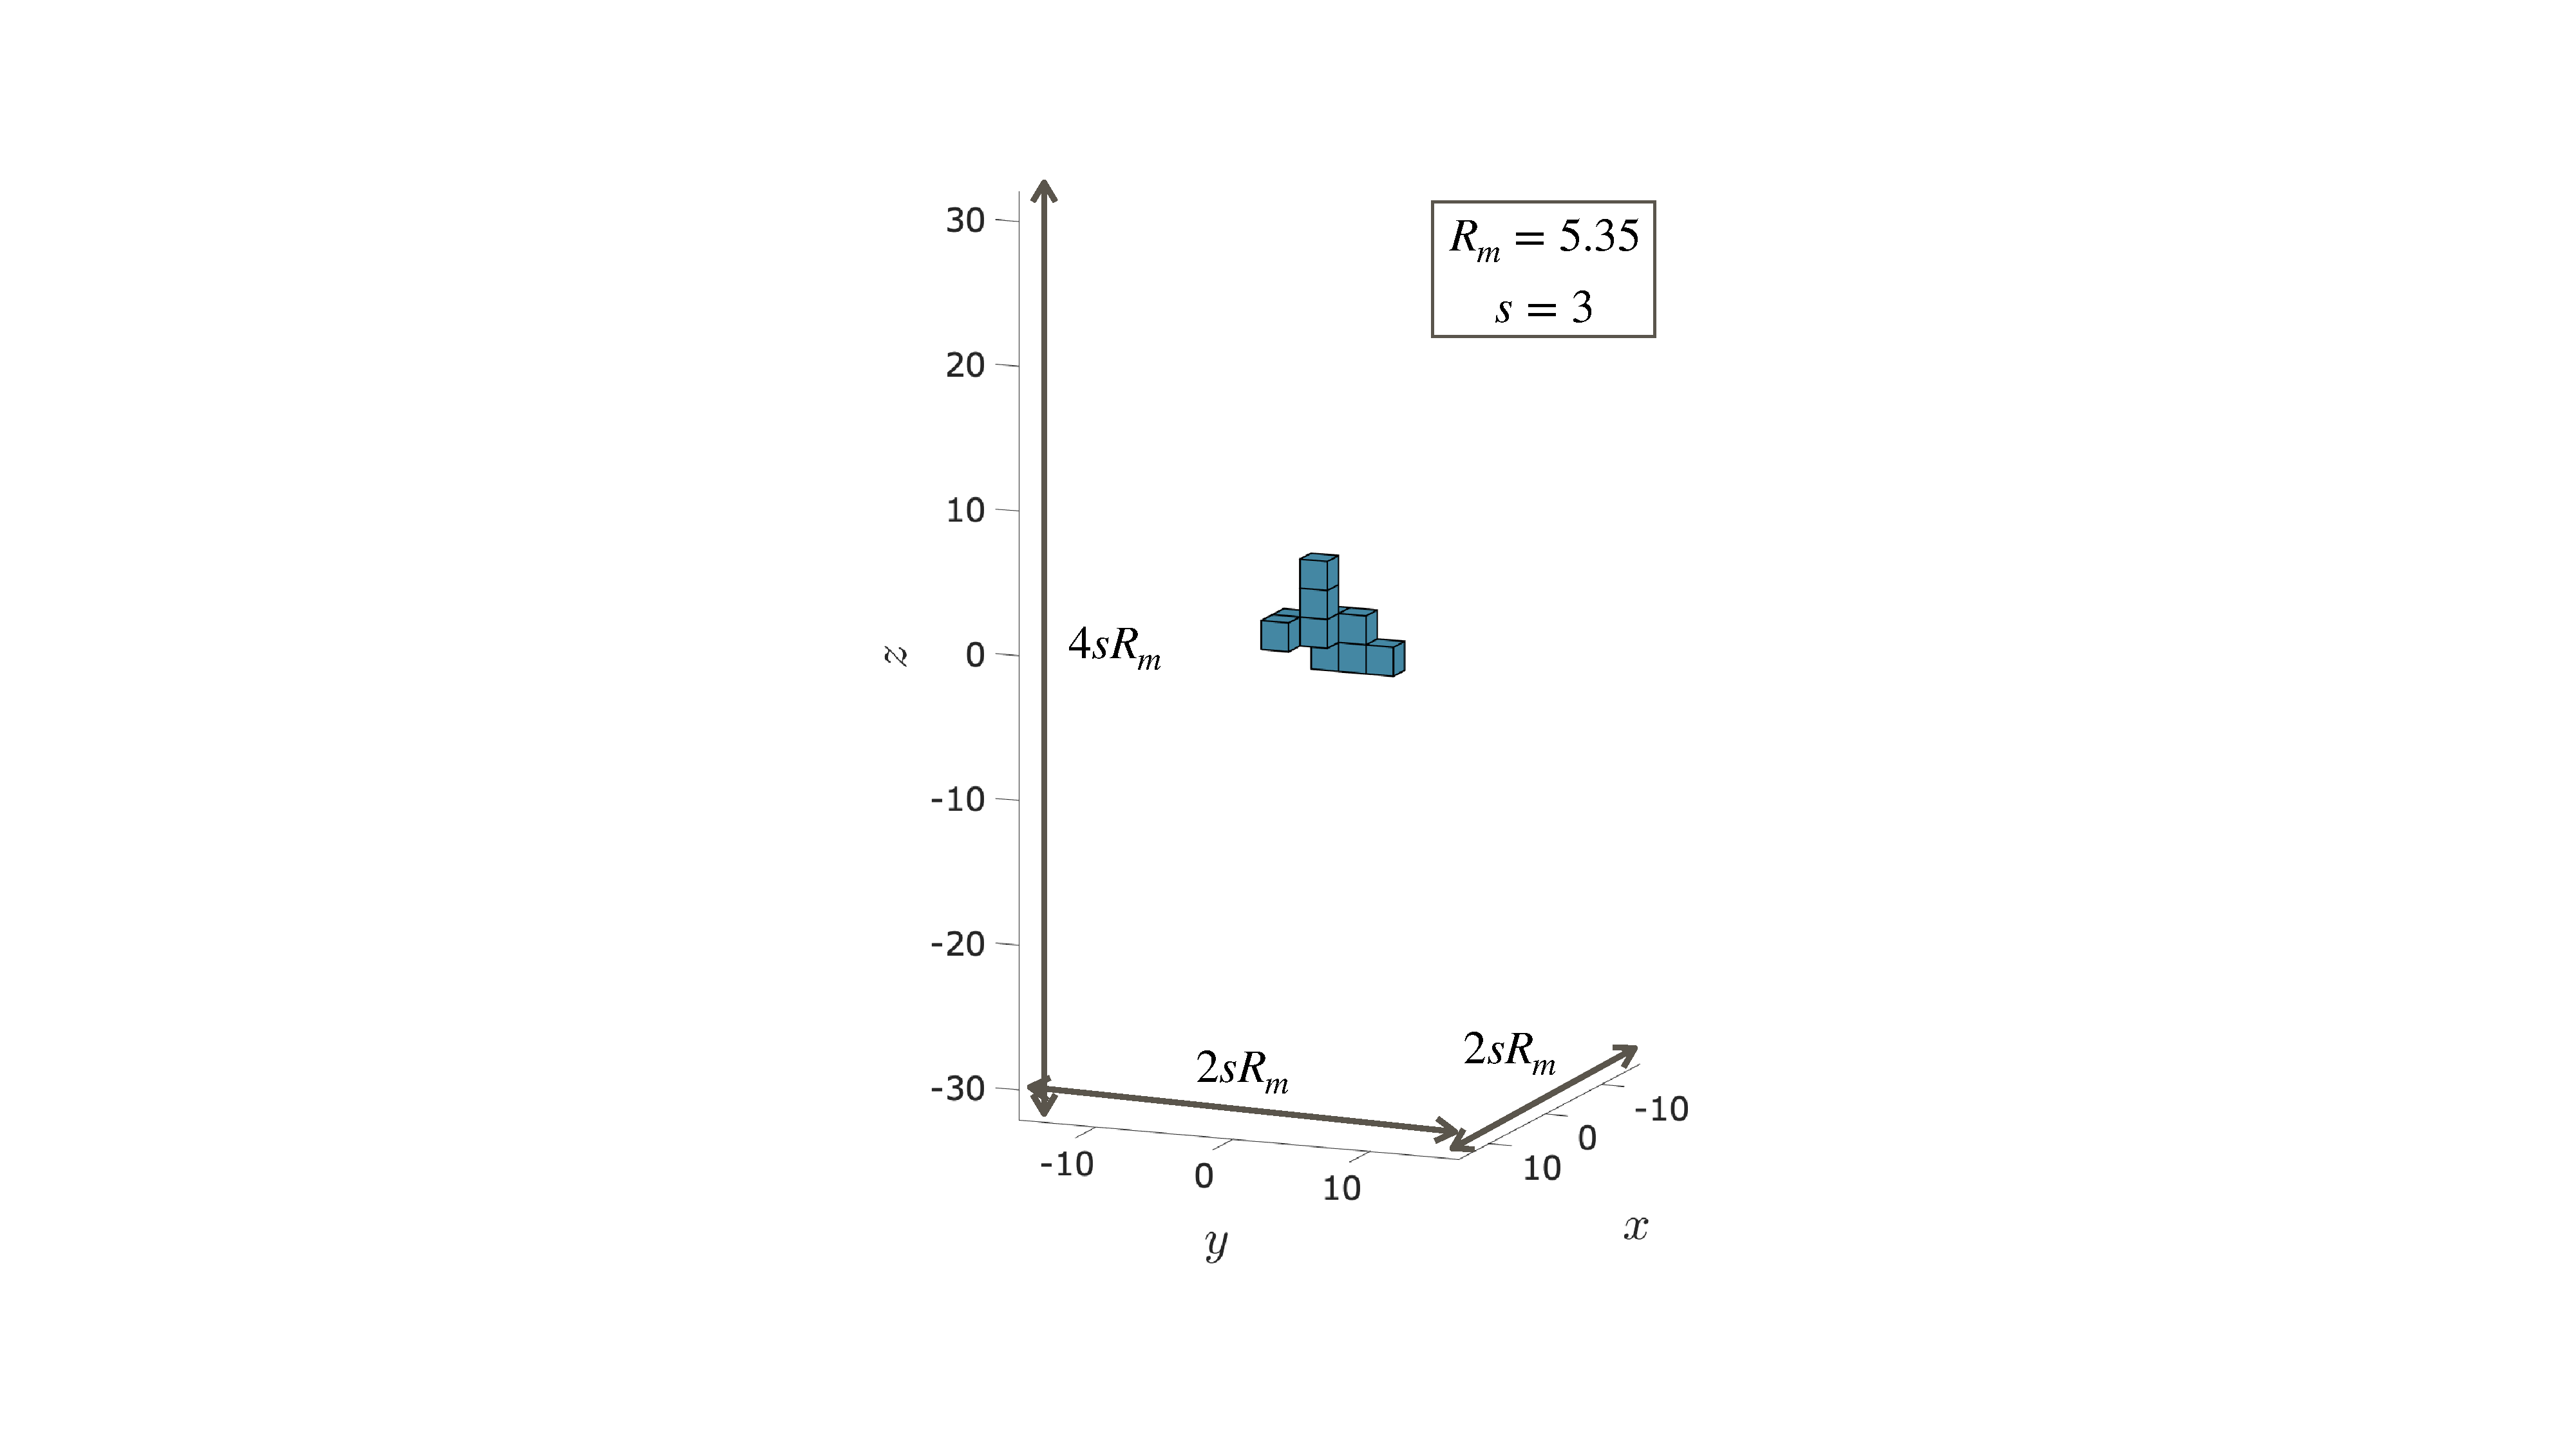
\includegraphics[scale=0.4]{./figures/fig_sample_agg10.pdf}
		\caption{Sample aggregate with ten cubes where $s = 3$, that is used to obtain simulations presented in Figure~\ref{fig_NC10_snaps_all}. }
		\label{fig_sample_agg10}
	\end{center}
\end{figure}
\par
Since we are interested in the aggregate's long-term settling behavior, we measure its (a) translational velocity $\vec{U}_a$, (b) location of $\vec{x}_{cm}$, and (c) drag $\vec{F}_o$ as a function of time. 
In particular, we present the vertical component of these three values, focusing on the settling direction.
We also want to observe the (d) perturbation $C(\vec{x},t)$. At locations far from the aggregate, we expect to see very small, almost zero, perturbation.
We thus focus on the perturbation value near the aggregate, denoted by $\vec{x}^{\star}$, which is distanced by approximately $(1.2 + R_m)$ from the center of mass. 
\par
\begin{figure}[ht]
	\begin{center}
		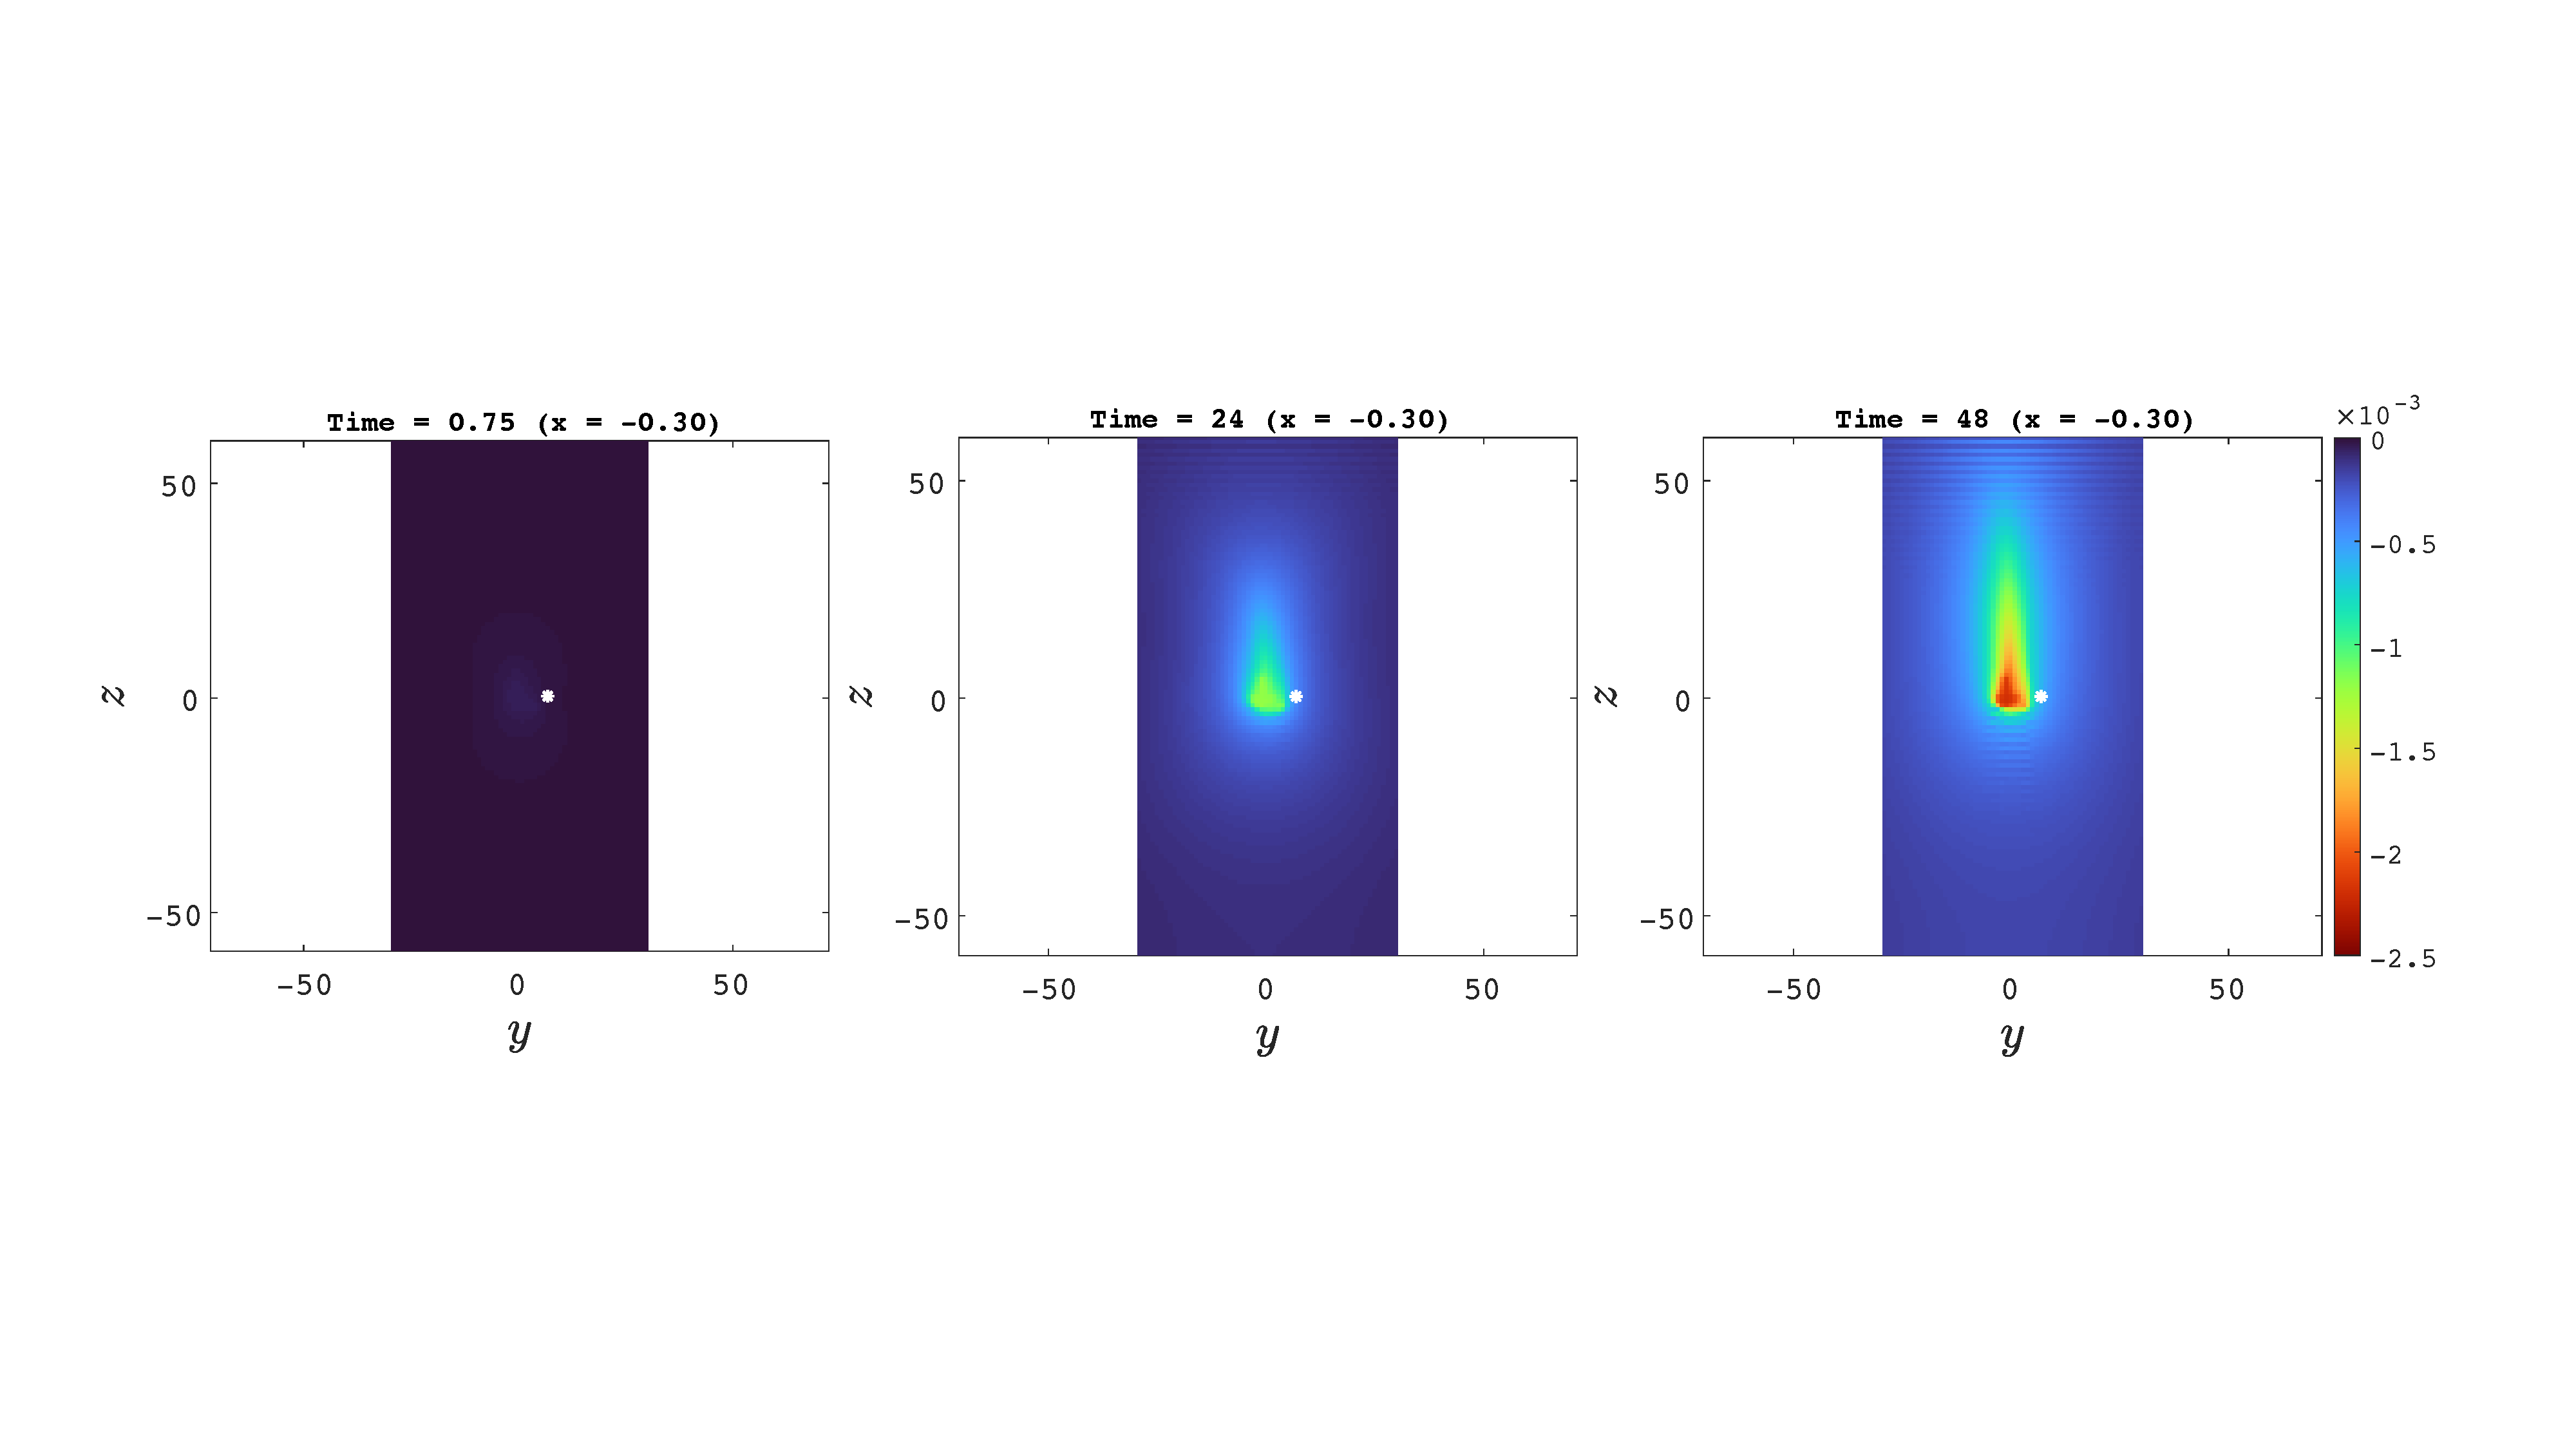
\includegraphics[scale=0.26]{./figures/fig_NC10_snaps_all.pdf}
		\caption{Snapshots of the perturbation obtained with $\Delta t = 0.75, \ \Delta x = 1,$ and $s = 5$. We look at the $y-z$ plane at $x = -0.3$, which is near the center of mass of the aggregate. The small white dot, $\vec{x}^{\star} = (-0.3, \ 6.9, \ 0.4)$, is located outside of, but very close to, the aggregate.}
		\label{fig_NC10_snaps_all}
	\end{center}
\end{figure}
We show three snapshots of the perturbation $C$ at three different times, obtained with $\Delta t = 0.75, \ \Delta x = 1$, and $s = 5$, at $x = -0.3$ as a sample result in Figure~\ref{fig_NC10_snaps_all}. Note that the white star point is at ${\vec{x}^{\star}} = (-0.3, \    6.9, \      0.4)$, which is the particular point at which we present $C$. Since we use the moving frame of reference to compute the perturbation, we see that the aggregate stays in the middle of the fluid domain in Figure~\ref{fig_NC10_snaps_all}.
We notice slight oscillations near the top of the fluid domain, where the zero-flux boundary condition is applied, as the perturbation increases. 
However, these oscillations remain relatively small and do not extend to the vicinity of the aggregate. 
We will consider a large enough fluid domain compared to the aggregate size, and study to observe the convergence of the quantities of interest, $\vec{U}_a(t), \ \vec{x}_{cm} (t), \ \vec{F}_o(t)$, and $C(\vec{x}^{\star}, t)$.
% -----subsection-------varying s----------
\subsection{Varying the domain size, via parameter $s$}
As we described in section~\ref{subsec:AD_numerics_space}, we have periodic boundary conditions in the horizontal direction to model an infinite domain where the velocity vanishes to zero. 
We seek to determine a domain size, via the multiplicative factor $s$, required to approximate these conditions.
If we can obtain reasonable results in a smaller domain, we could use smaller $s$ that results in more rapid computations and smaller memory requirements. 
\begin{figure}[ht]
	\begin{center}
		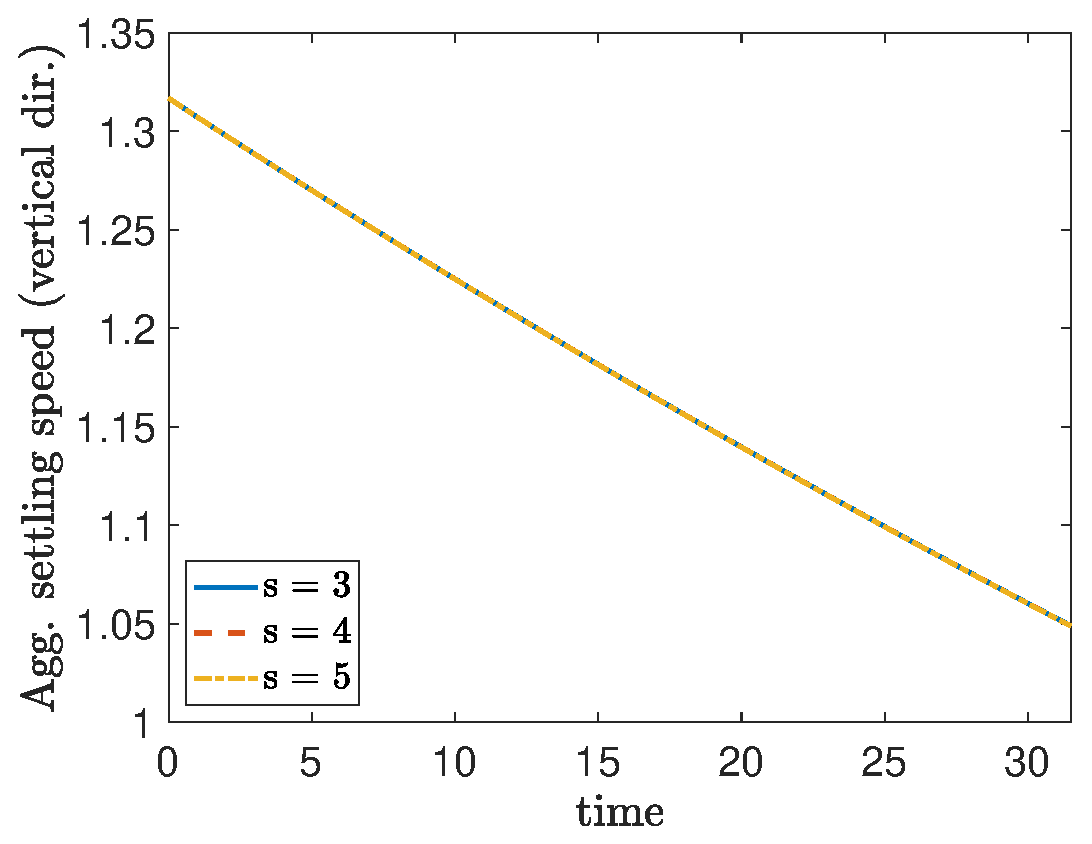
\includegraphics[scale=0.35]{./figures/fig_NC10_s_Ua3_all}
		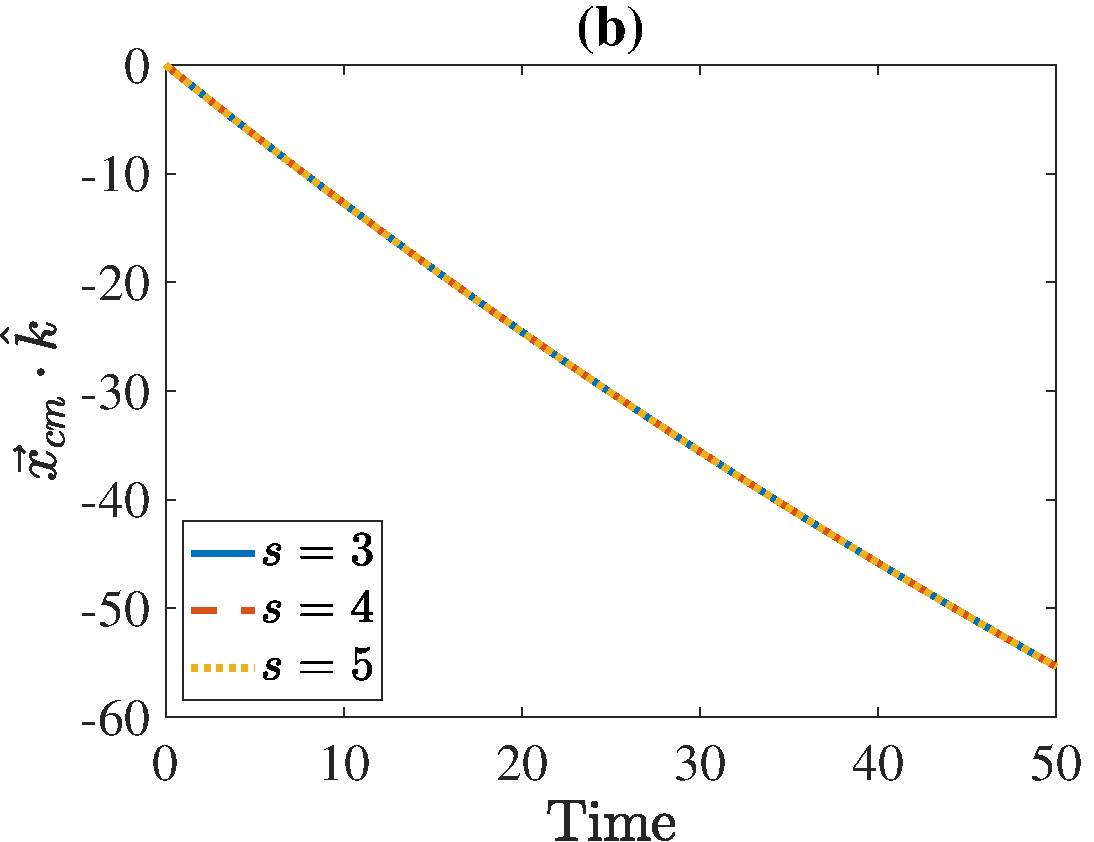
\includegraphics[scale=0.35]{./figures/fig_NC10_s_cm3_all}
		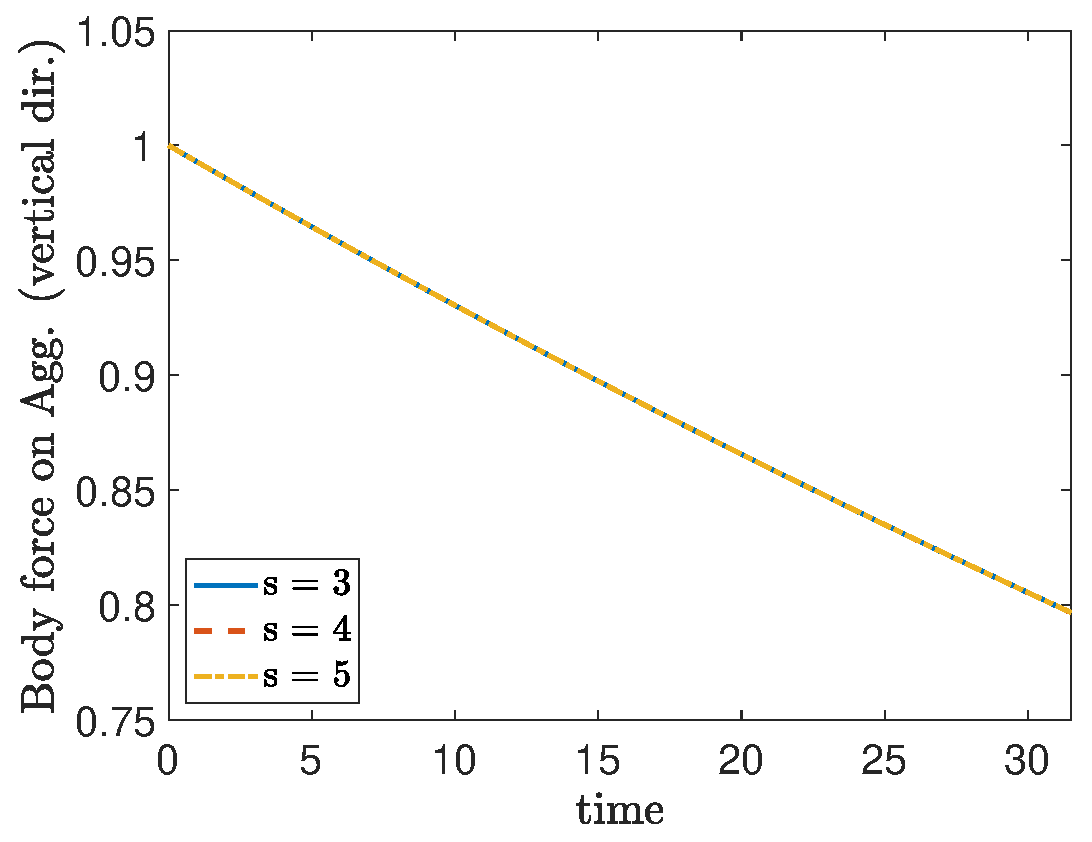
\includegraphics[scale=0.35]{./figures/fig_NC10_s_Fo3_all}
		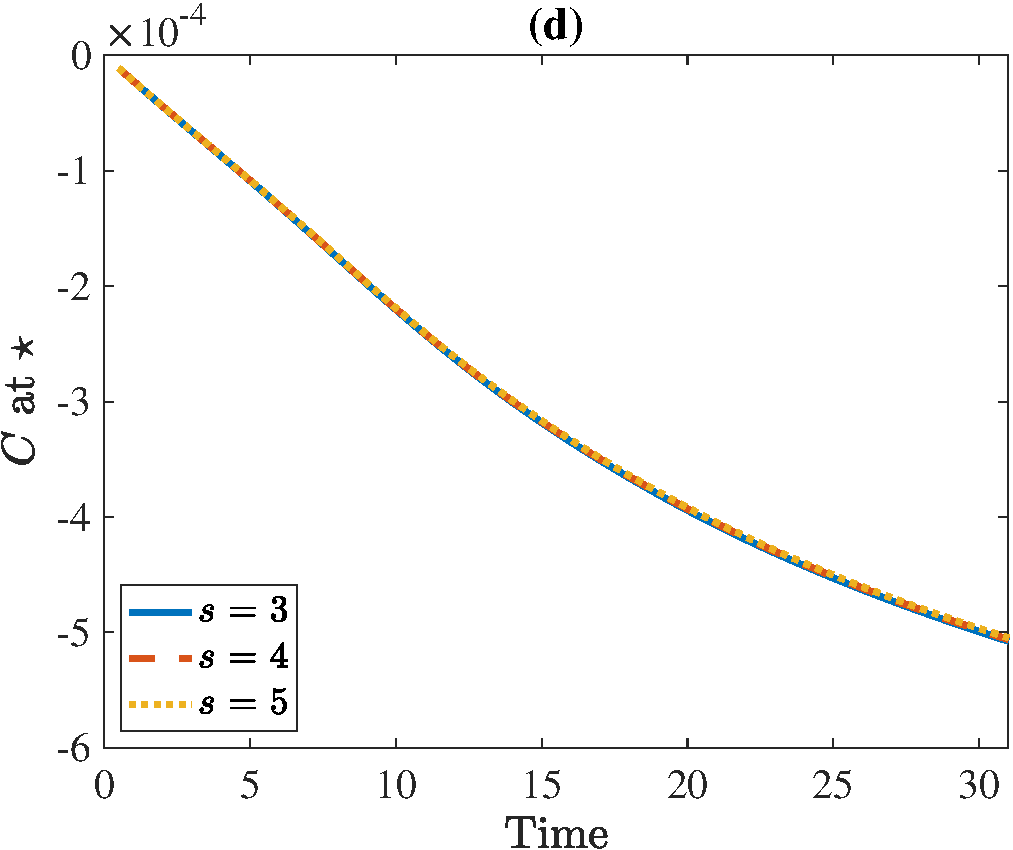
\includegraphics[scale=0.35]{./figures/fig_NC10_s_C_star}
	\caption{Comparison of various domain sizes with $ s = 3, \ 4, \ 5$. The time step is $\Delta t = 0.5$ and the grid size is $\Delta x = 1$. We show (a) the settling speed, (b) the position of the center of mass, (c) the vertical force on the aggregate, and (d) the value of the perturbation at $\vec{x}^{\star}$. Note that $NC = 10$ is the number of cubes used to form the aggregate.}
	\label{fig_NC10_compare_s}
\end{center}
\end{figure}
\par
In Figure~\ref{fig_NC10_compare_s}, we present three different domain sizes with the $s$ factor $s = 3, \ 4$, and $5$. At first glance, we can barely tell the differences between all three cases. In other words, there is no significant impact on aggregate behavior when reducing the domain size down to $s = 3$. Although we notice that the perturbations at $\vec{x}^{\star}$ show a little more variation with $s$, this remains a negligible effect.

\subsection{Varying time step, $\Delta t$}
We now vary the time step, $\Delta t$. We consider three different cases, $\Delta t = 0.75, \ 0.5$, and $0.25$. We are able to run simulations with somewhat large time steps since the aggregate size is small enough to have a velocity of order one. When the initial settling velocity is high, the CFL condition (\ref{eq_CFL}) can be violated, leading to instability. As the aggregate settles, the surrounding fluid becomes denser, which decreases the velocity, and therefore the CFL number. Thus, the velocities are more limiting on the time step at the beginning of the simulation. 
\par
While we vary $\Delta t$, we set the domain size to aggregate diameter ratio $s = 3$ since we observed no critical changes in aggregate dynamics and we can save on computational time. For a fair comparison, we keep the grid size $\Delta x =1$. 
The main takeaway of Figure~\ref{fig_NC10_compare_dt} is that there are no significant differences in the values we observe when we vary $\Delta t = 0.75, \ 0.5$, and $0.75$. Once again, we notice some variations in the perturbation $C(\vec{x}^{\star},t$ at later times. 
However, these remain smaller than 4\%.
\begin{figure}[ht]
	\begin{center}
		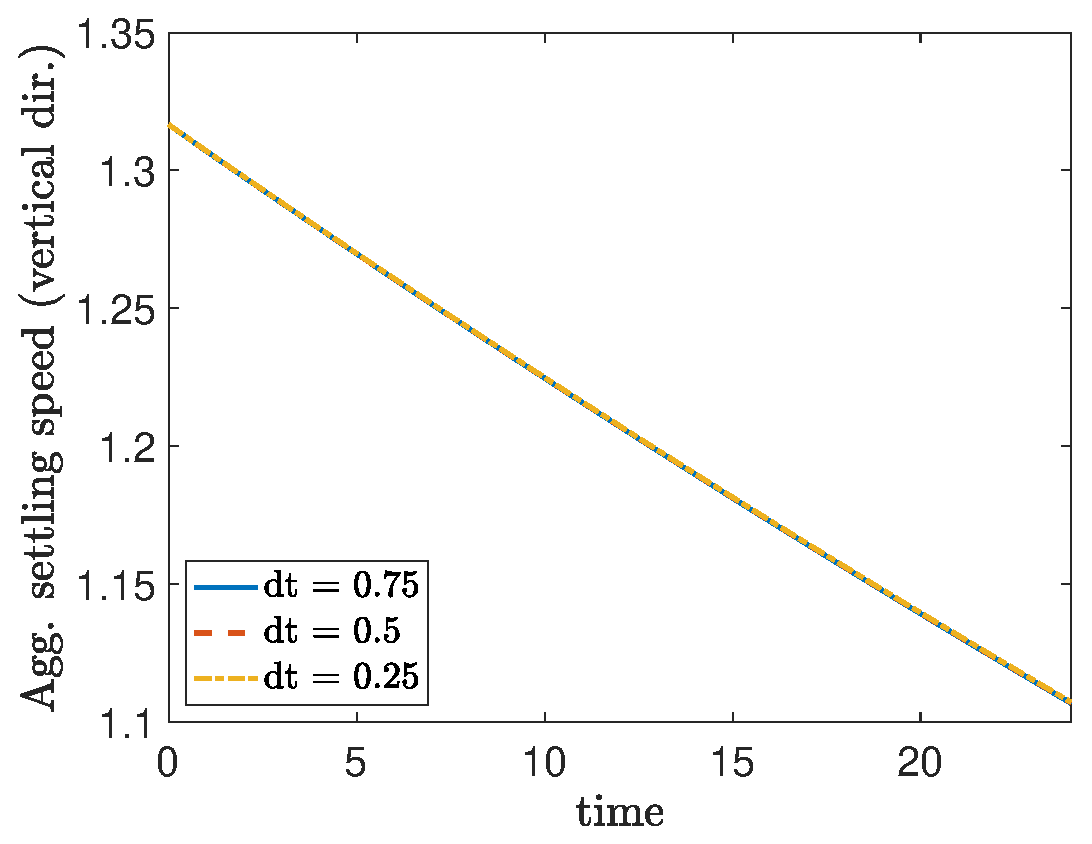
\includegraphics[scale=0.35]{./figures/fig_NC10_dt_Ua3_all}
		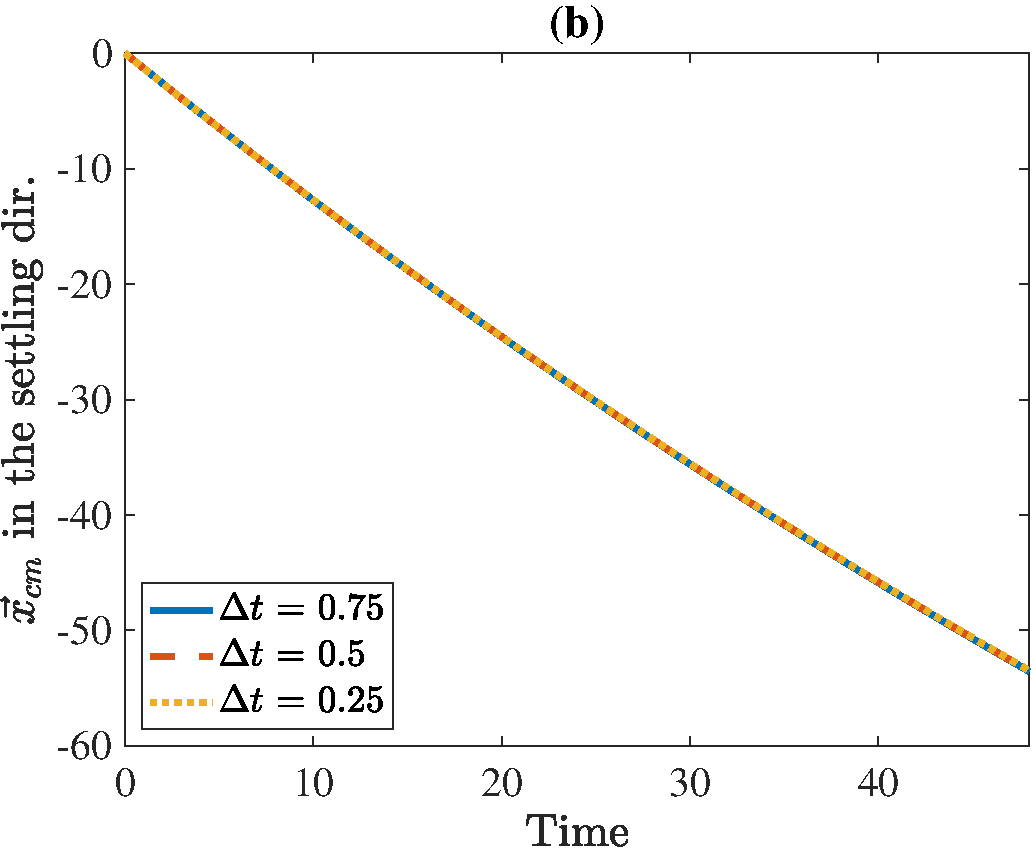
\includegraphics[scale=0.35]{./figures/fig_NC10_dt_cm3_all}
		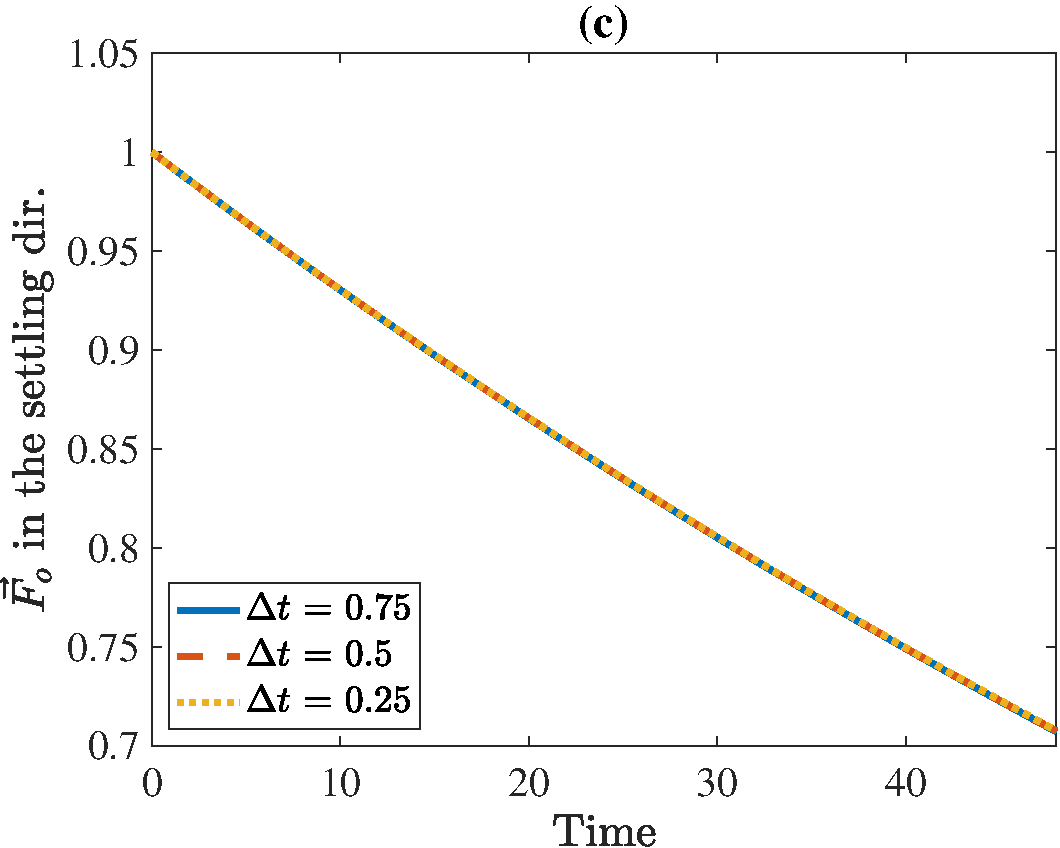
\includegraphics[scale=0.35]{./figures/fig_NC10_dt_Fo3_all}
		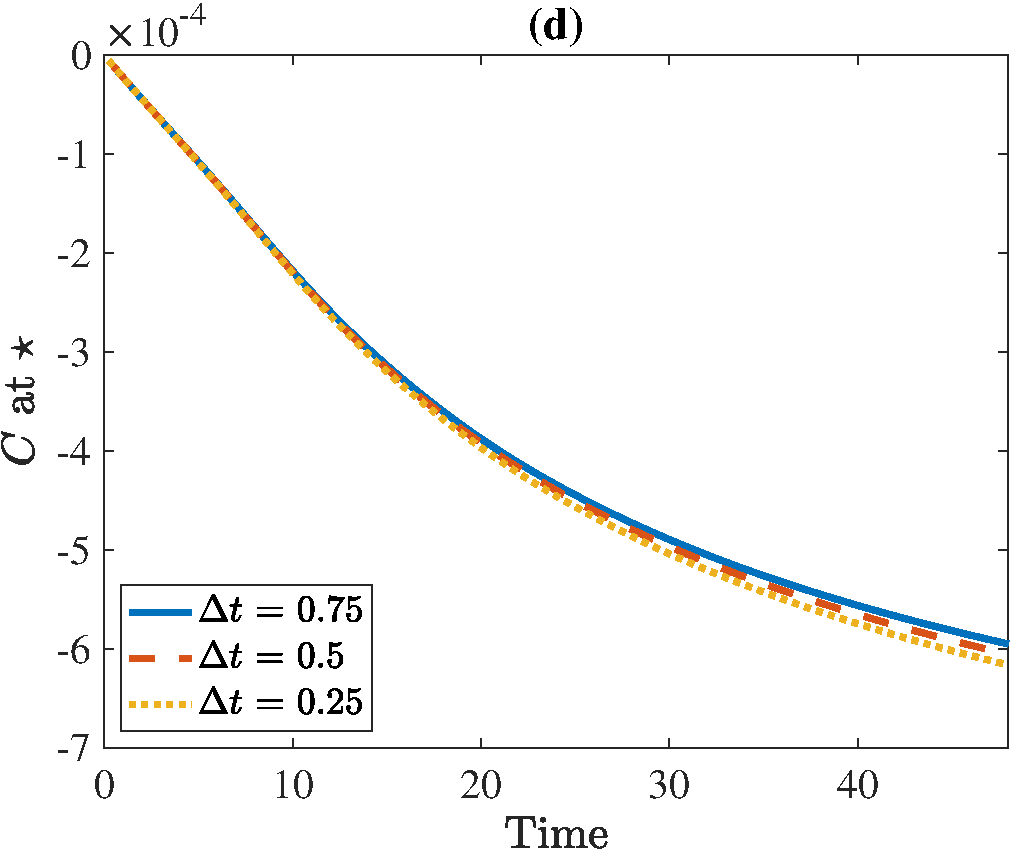
\includegraphics[scale=0.35]{./figures/fig_NC10_dt_C_star}
	\caption{Comparison of various $\Delta t = 0.75, \ 0.5, \ 0.25$ in the domain size factor $s = 5$ with $\Delta x = 1$. We show (a) the settling speed, (b) the position of the center of mass, (c) the vertical force on the aggregate, and (d) the value of the perturbation near the aggregate.}
	\label{fig_NC10_compare_dt}
\end{center}
\end{figure}
\par
To more accurately capture the effects of varying $\Delta t$, we also present the relative errors between two $\Delta t = 0.25$ and $0.5$ in Figure~\ref{fig_NC10_dt_err_all}.
It is clear that the errors in all four values are fairly small compared to the error at the corner we found in section~\ref{subsec:FMM} (due to the approximation of constant stress over each face). For the time integration scheme we use, which is the explicit RK2 method, we typically expect to have second-order convergence. These error plots support that our solutions have reached convergence.
\begin{figure}[h]
	\begin{center}
		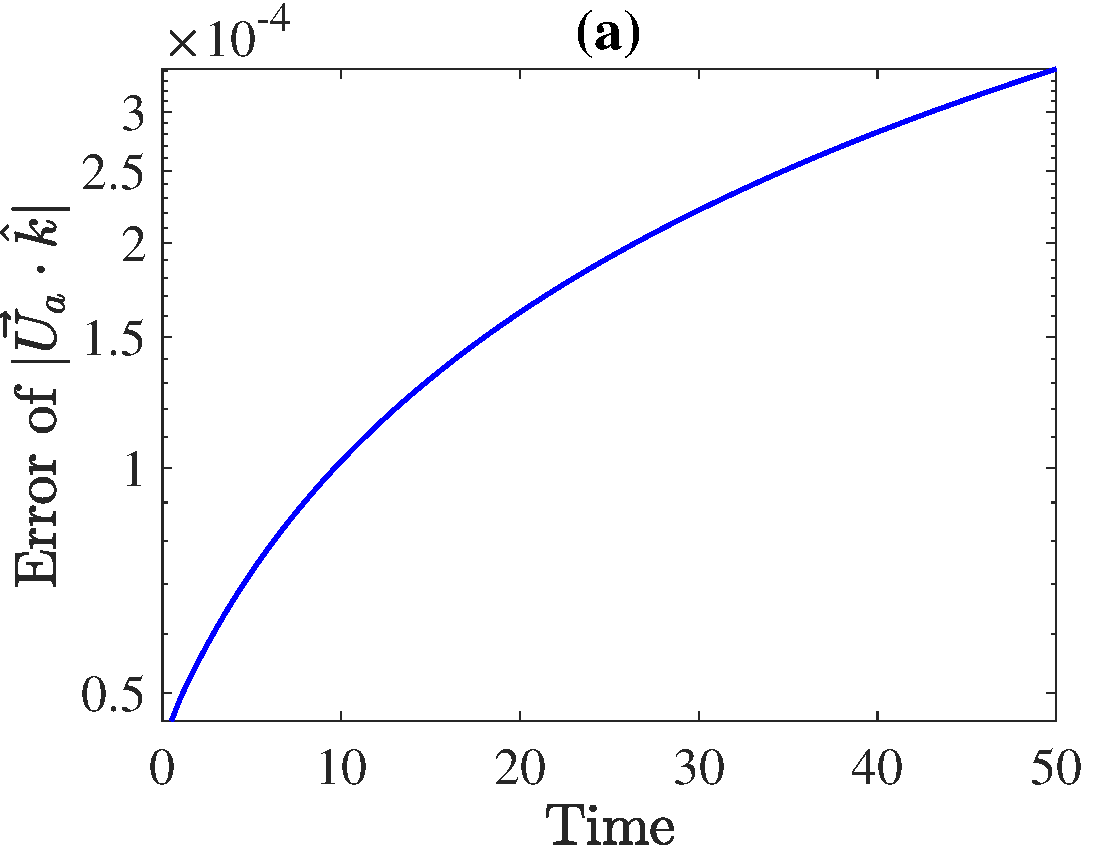
\includegraphics[scale=0.35]{./figures/fig_NC10_dt_err_Ua3_all}
		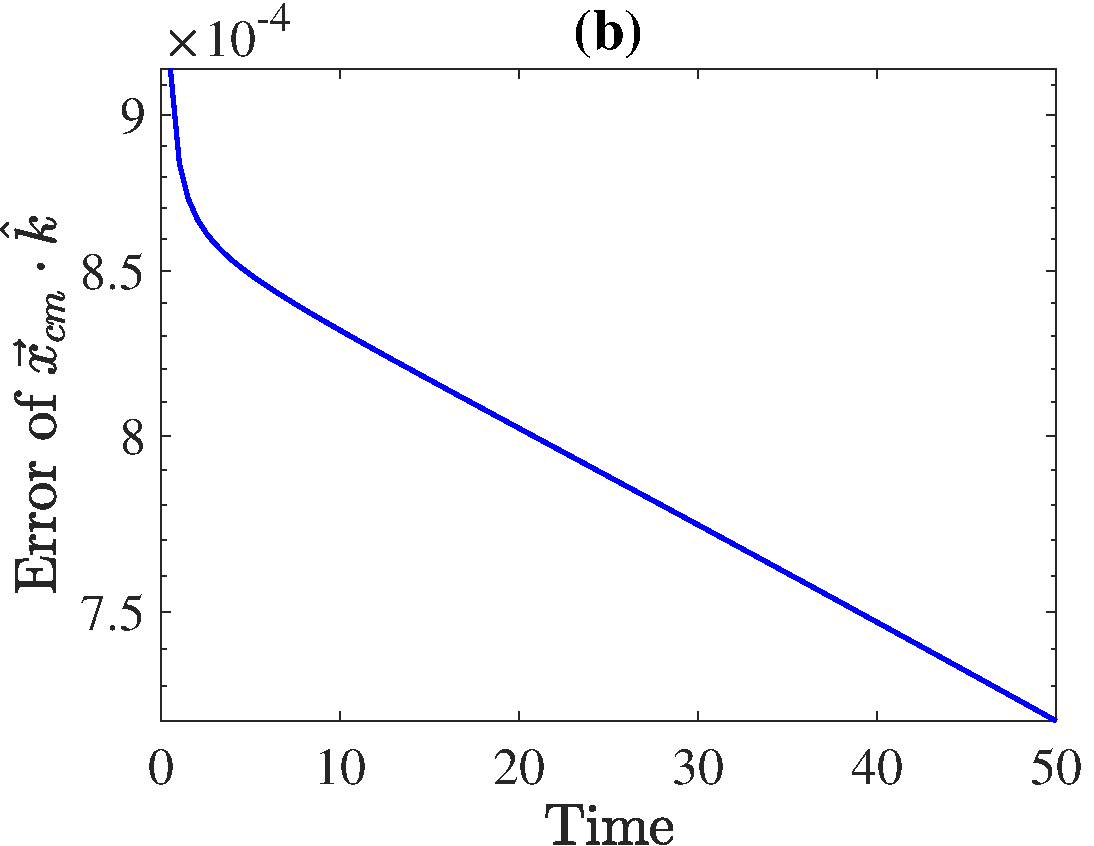
\includegraphics[scale=0.35]{./figures/fig_NC10_dt_err_cm3_all}
		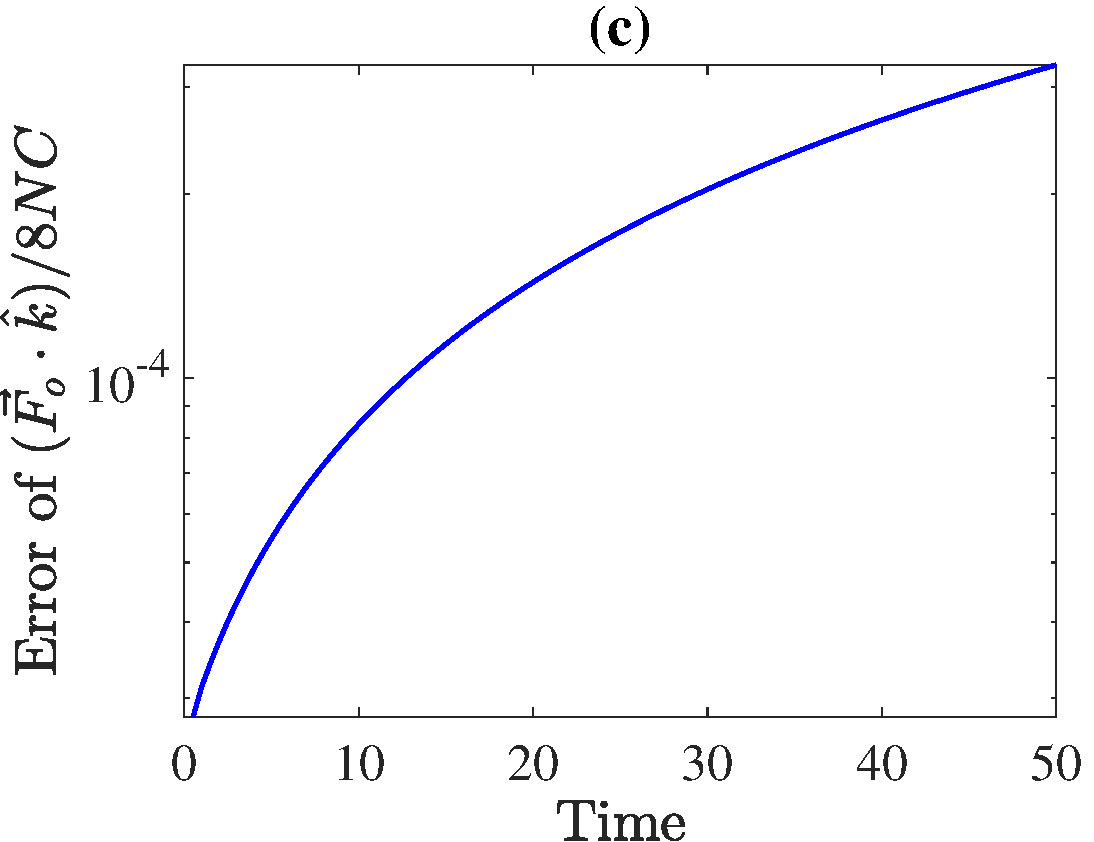
\includegraphics[scale=0.35]{./figures/fig_NC10_dt_err_Fo3_all}
		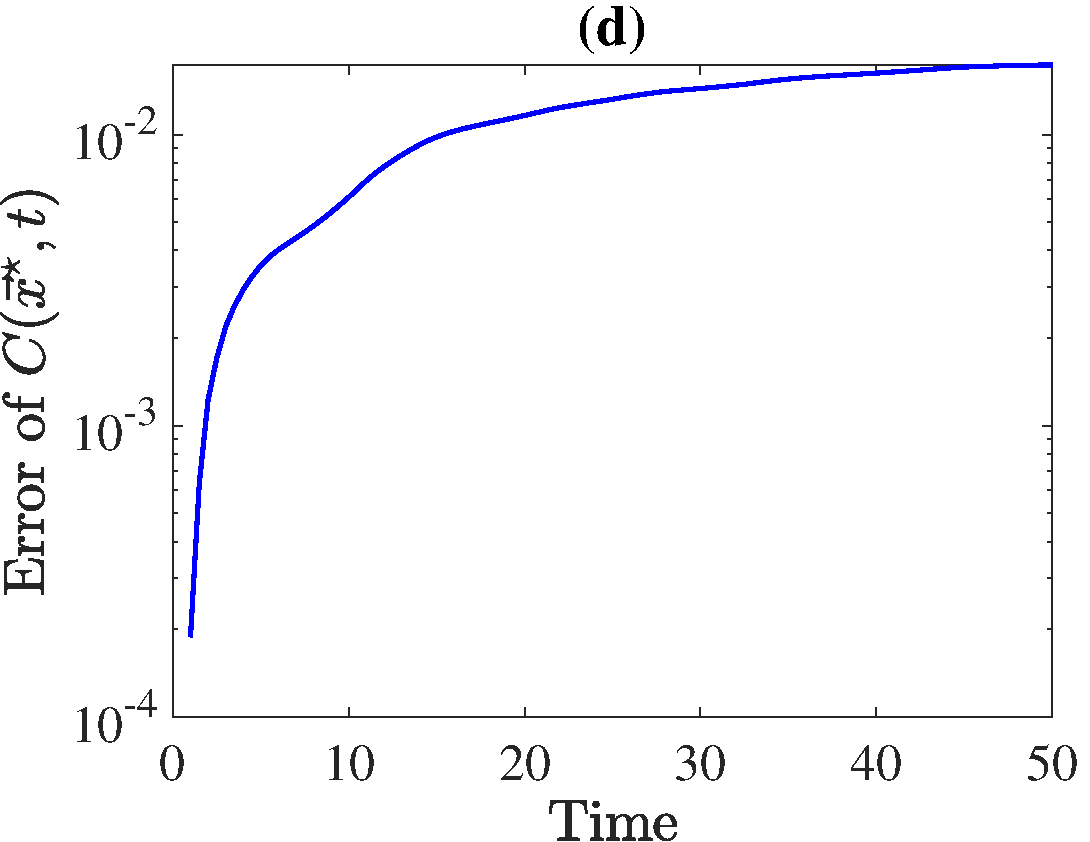
\includegraphics[scale=0.35]{./figures/fig_NC10_dt_err_C_star}
	\caption{Relative error between $\Delta t = 0.5$ and 0.25 cases.}
	\label{fig_NC10_dt_err_all}
\end{center}
\end{figure}

\subsection{Varying grid size, $\Delta x$}
Lastly, we perform the simulations with several grid sizes, $\Delta x = 1, \ 2, $ and $4$. 
The choice of such large grid sizes is justified by the approximation of constant stress over each face (of side length 2).
In general, as long as all three choices produce similar results and have no stability issues, we prefer to use as large $\Delta x$ as possible to reduce the computational time. 
The number of fluid grid points can also be a challenge in terms of computational memory required. 
\par
\begin{figure}[ht]
	\begin{center}
		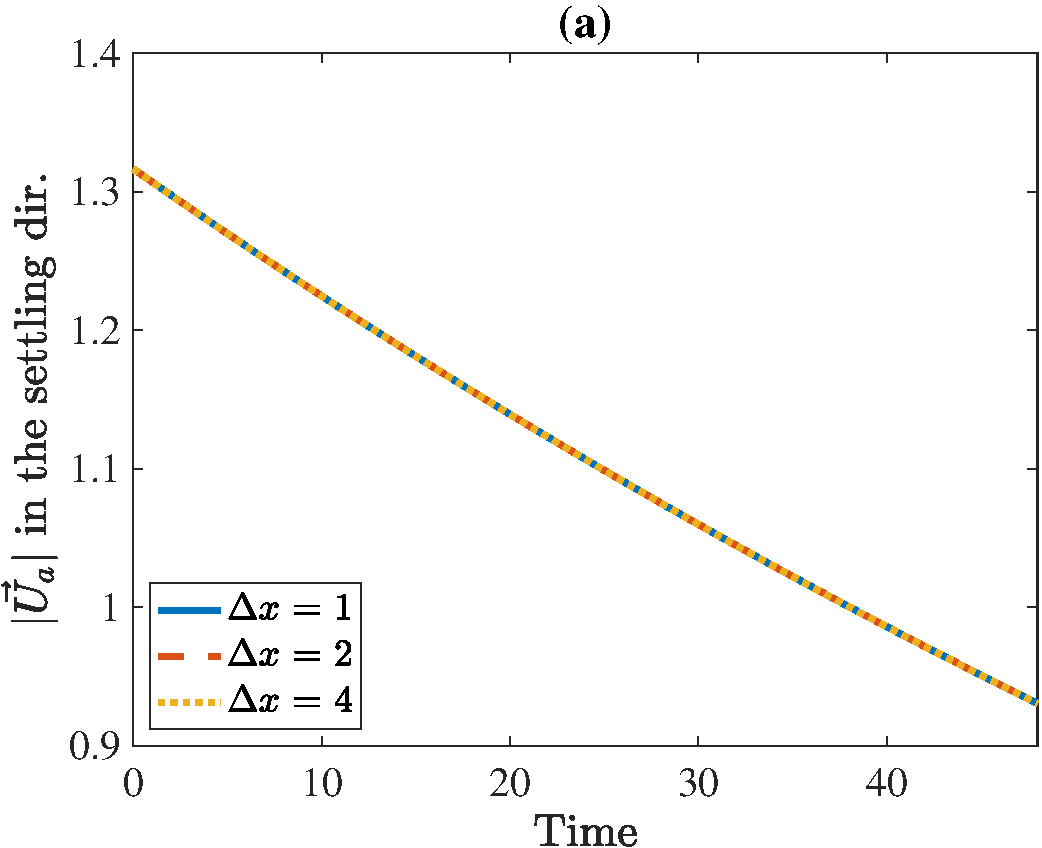
\includegraphics[scale=0.35]{./figures/fig_NC10_dx_Ua3_all}
		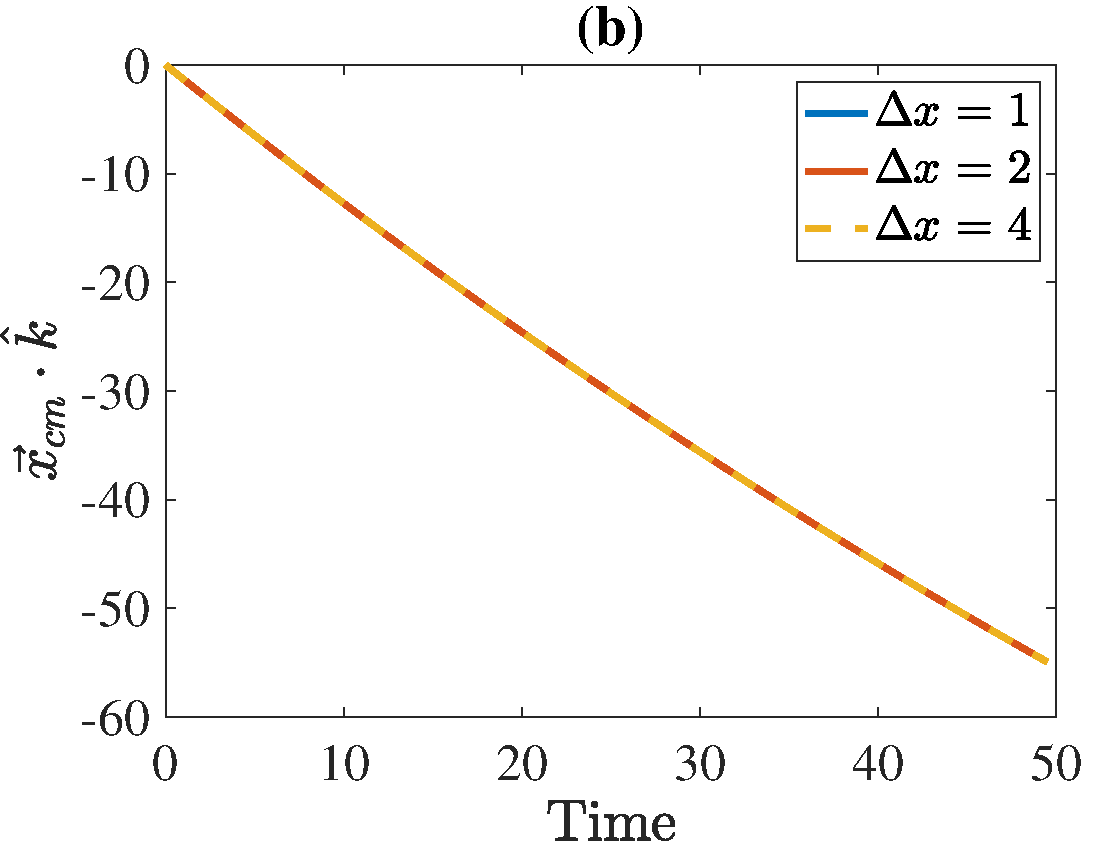
\includegraphics[scale=0.35]{./figures/fig_NC10_dx_cm3_all}
		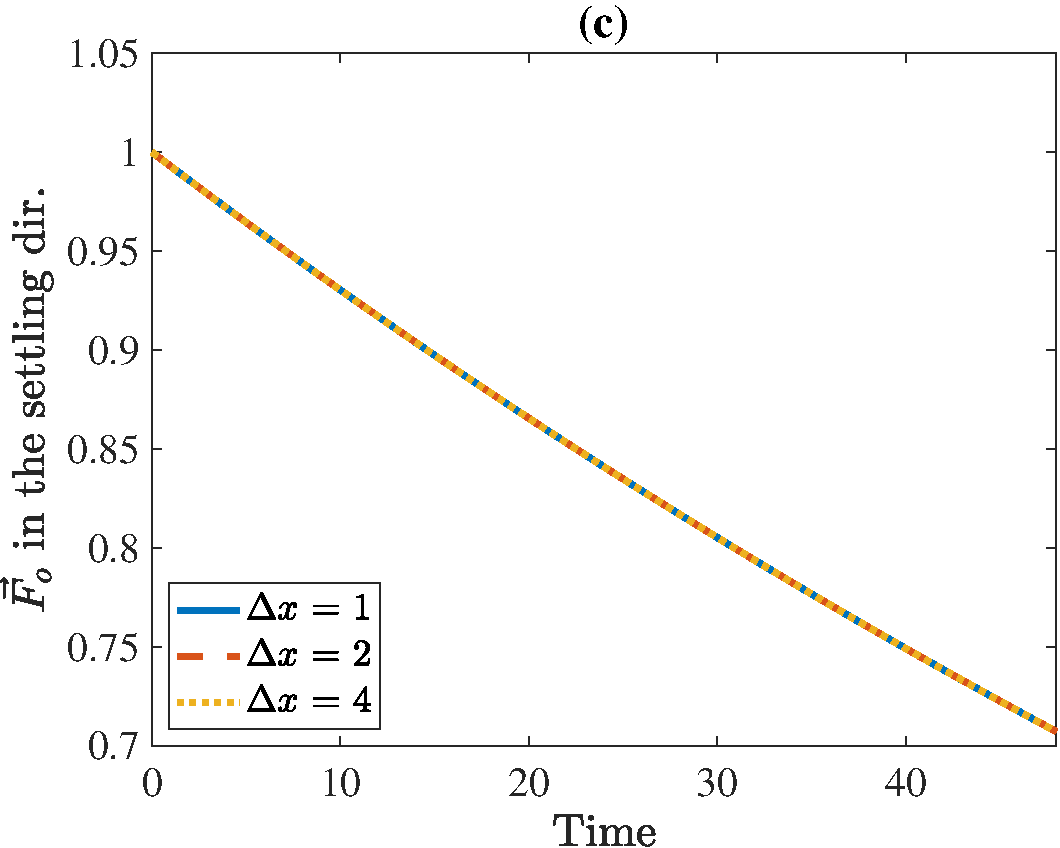
\includegraphics[scale=0.35]{./figures/fig_NC10_dx_Fo3_all}
		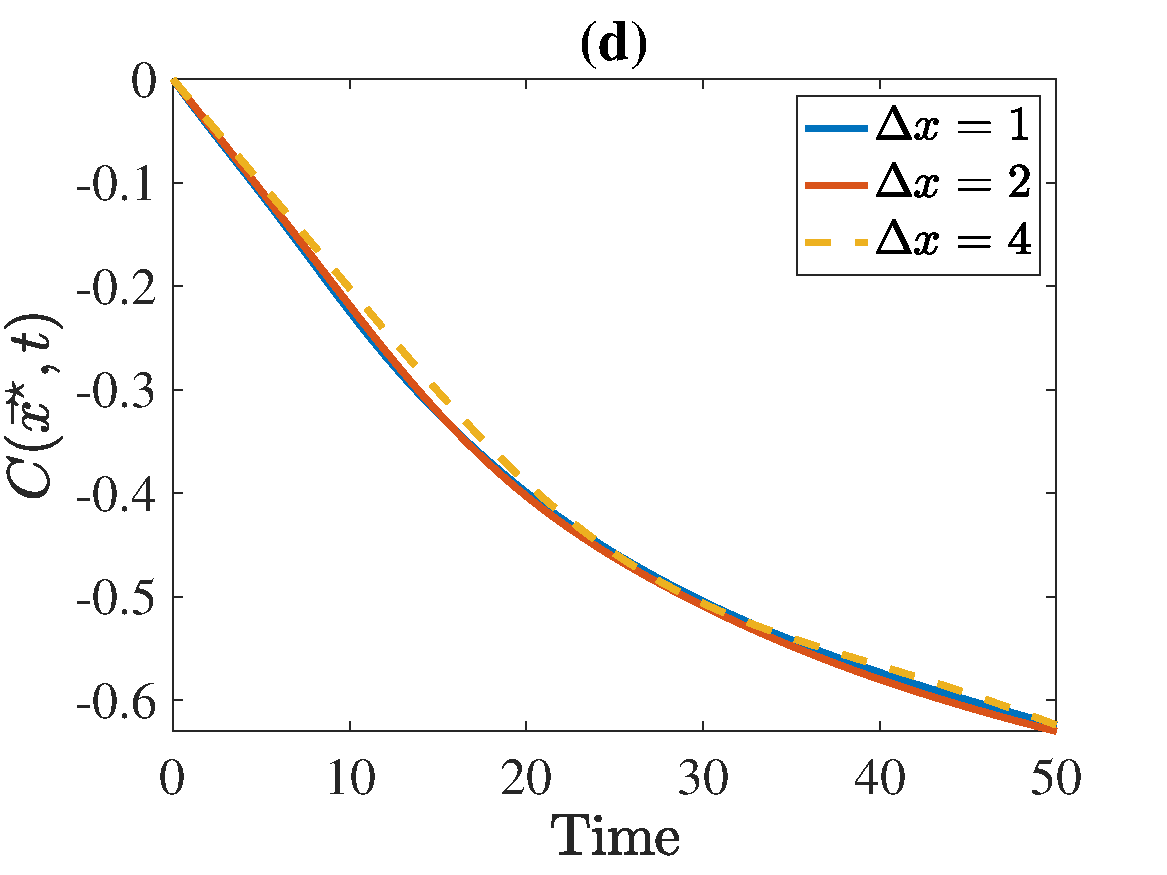
\includegraphics[scale=0.35]{./figures/fig_NC10_dx_C_star_interp3}
	\caption{Comparison of various $\Delta x = 1, \ 2, \ 4$ in the domain size factor $s = 5$ with $\Delta t = 0.75$. We show (a) the settling speed, (b) the position of the center of mass, (c) the vertical force on the aggregate, and (d) the he value of the perturbation near the aggregate.}
	\label{fig_NC10_compare_dx}
\end{center}
\end{figure}
As we saw in the first two validations, we observe quite good agreement presented in the velocity, location, and drag, in Figure~\ref{fig_NC10_compare_dx}. If we had computation time or memory capacity constraints, these results in plots (a), (b), and (c) support that we can still obtain qualitative results to analyze a settling aggregate. 
\par
For the last plot (d), since we have different grid spacings, we were not able to capture the perturbation at the $\vec{x}^{\star}$ exactly for $\Delta x = 2$ and 4 cases.  
We thus used MATLAB built-in function \verb+interp3+ to interpolate the $C$ value at location $\vec{x}^{\star}$. We particularly select the nearest-neighbor method, which finds the value at the nearest sample grid point. We find the interpolation results seem to be reliable, having a good match with previous results of $C$ with various domain and time step sizes. 

% As we plan to use approximately 10 times larger aggregate to show the results in section~\ref{sec:stratified_results}, it is inevitable to adjust both grid and time step sizes. 
\par
\vphantom{D}
\par
Before we conclude this section, we want to note that it is difficult to say we obtained the correct solution since we do not have any analytic solutions. The validations we provide here are to exhibit convergence and estimate the size of the errors made due to time and space discretization and finite domain size effects.
The results we described in this section were confirmed with simulations of an aggregate made with 50 cubes, and similar trends were observed. We present larger aggregate model simulations in the next section.
%-----RESULTS-----------------------------
\section{Simulation results}
\label{sec:stratified_results}
\subsection{Base case analysis}
Since there are several parameters we are interested in varying, we decide on setting a base case to compare further simulations. To explore assorted shapes, we use 50 cubes to form an aggregate. We particularly use the aggregate shape in Figure~\ref{fig_NC50_base_seed2}. 
\begin{figure}[ht]
	\begin{center}
		\vspace*{3mm}
		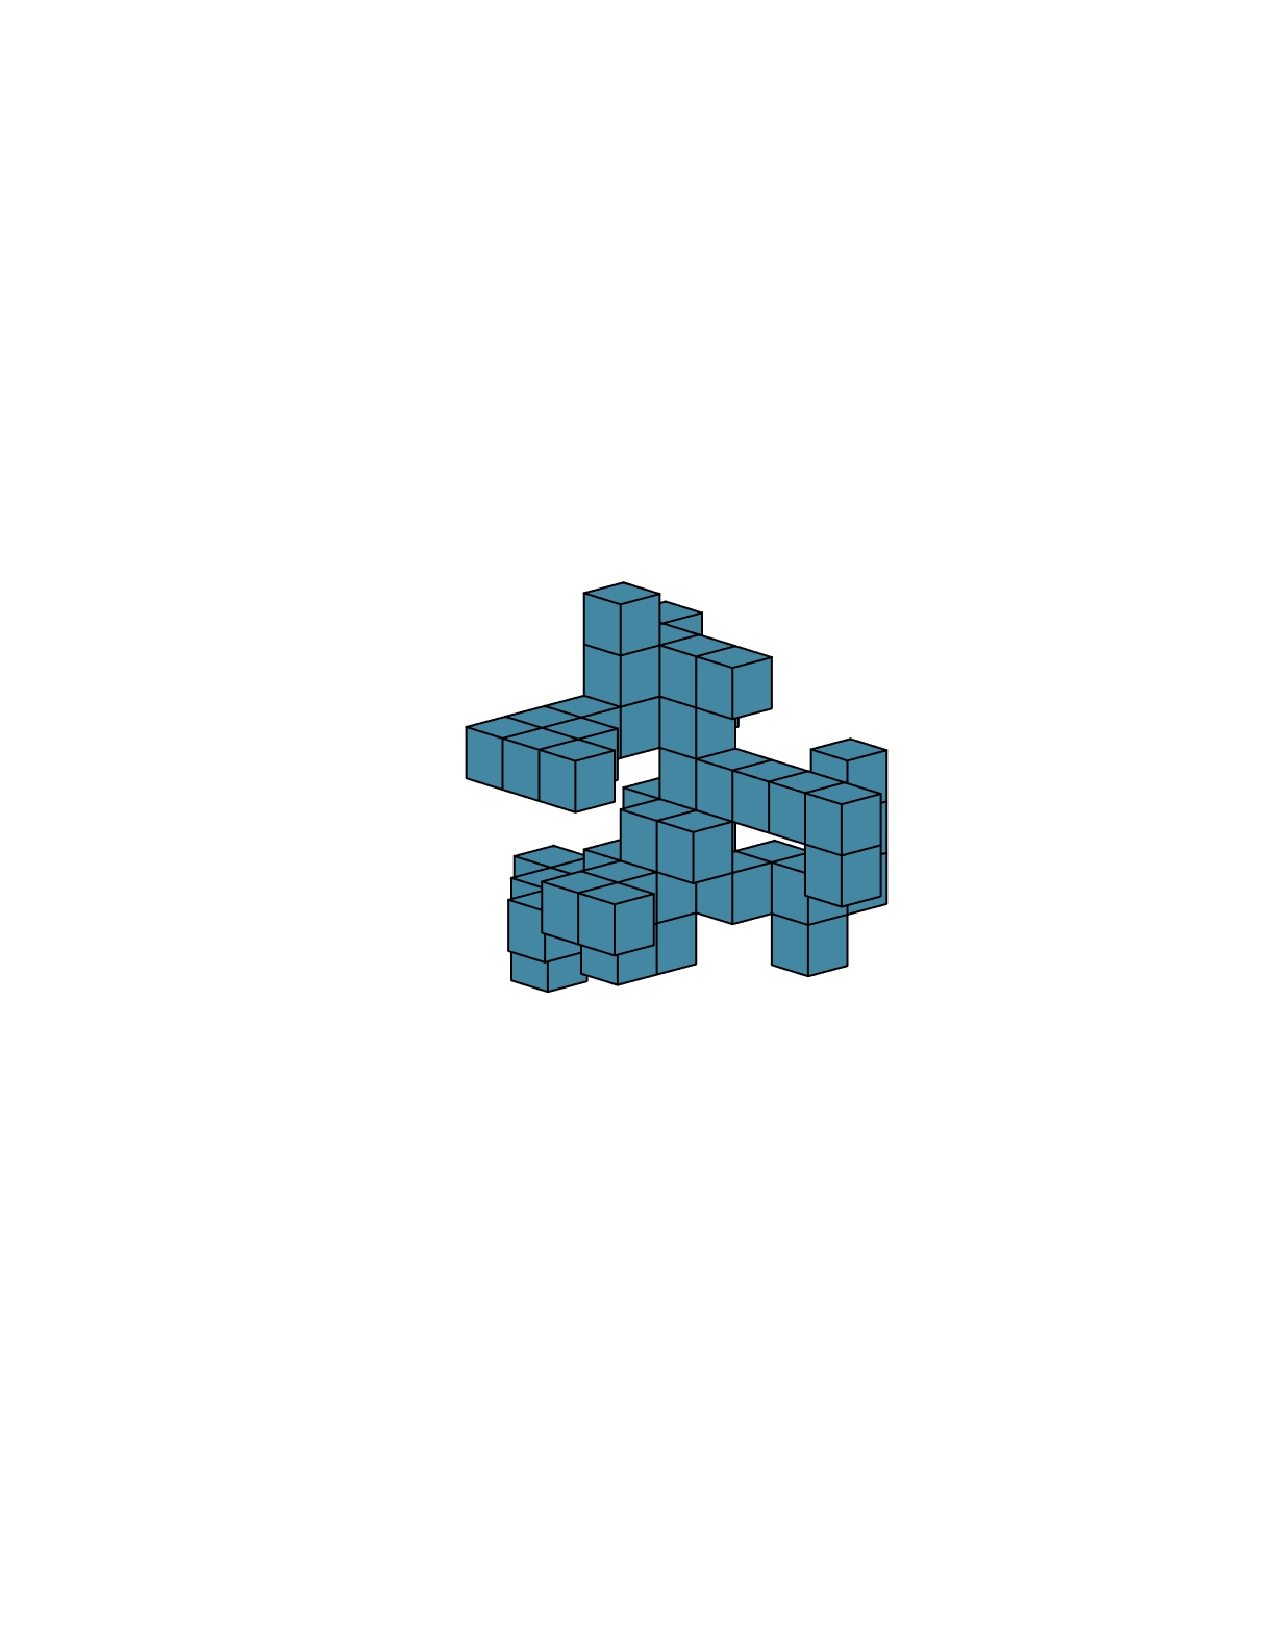
\includegraphics[scale=0.5]{./figures/fig_NC50_seed2}
	\caption{The base aggregate model (random seed number 2) with 50 cubes.}
	\label{fig_NC50_base_seed2}
\end{center}
\end{figure}
To avoid any stability issues while being computationally efficient, we choose the time step size $\Delta t = 0.5$ and grid spacing $\Delta x =1$. In section~\ref{sec:ch3_validation}, we have shown that these choices provide good accuracy. Moreover, we found that simulating the settling aggregate in the domain size with the scaling factor $s = 3$ is sufficient to have negligible boundary effects.  Also, we apply Pe = 100 as we did for the homogeneous model in Chapter~\ref{sec:ch2_CO2_simulation} for this base model.
\begin{figure}[ht]
	\begin{center}
		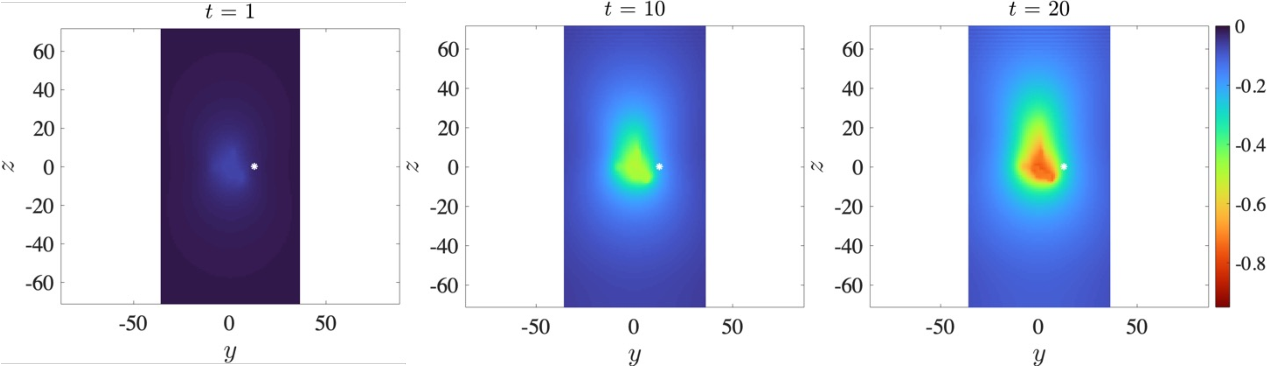
\includegraphics[scale=0.65]{./figures/fig_NC50_snaps_pt1.pdf}
		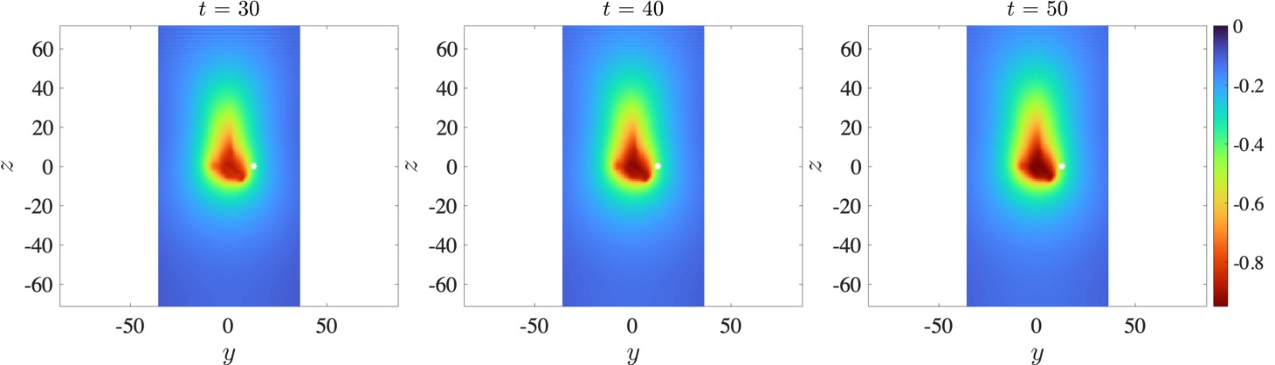
\includegraphics[scale=0.65]{./figures/fig_NC50_snaps_pt2.pdf}
	\caption{Concentration dynamics with the base model case at various times.}
	\label{fig_NC50_snaps_all}
\end{center}
\end{figure}
\par
Additionally, we select the stratification strength $\gamma$ more systematically. 
To do so, we first consider the settling distance of an aggregate, denoting it as $z_T$. In Figure~\ref{fig_sample_agg10}, we show that the aggregate is initially located in the middle of the domain. We are interested in observing a setup where $\gamma$ is as large as possible while allowing the aggregate to travel about $z_T = 6R_a$, before
reaching its level of neutral buoyancy.
Equation (\ref{eq_rho_bg}) allows us to compute the background fluid stratification $\gamma$
\begin{equation}
	\rho_{bg} = \rho_0 (1-\gamma z_T) =	\rho_0 (1 - \gamma 6R_a ) = \rho_a.
	\label{eq_compute_G}
\end{equation}
We want the aggregate density $\rho_a$, which is defined in equation (\ref{eq_rho_a}), to reach neutral buoyancy, assuming its fluid portion $\rho_f$ is $\rho_0$.
For an aggregate composed of 50 cubes, we have an estimated average radius $R_a \approx 9$~\cite{yoo_hydrodynamic_2020}, and thus we find $\gamma \approx 4 \times 10^{-4}$.  
\begin{figure}[h]
	\begin{center}
		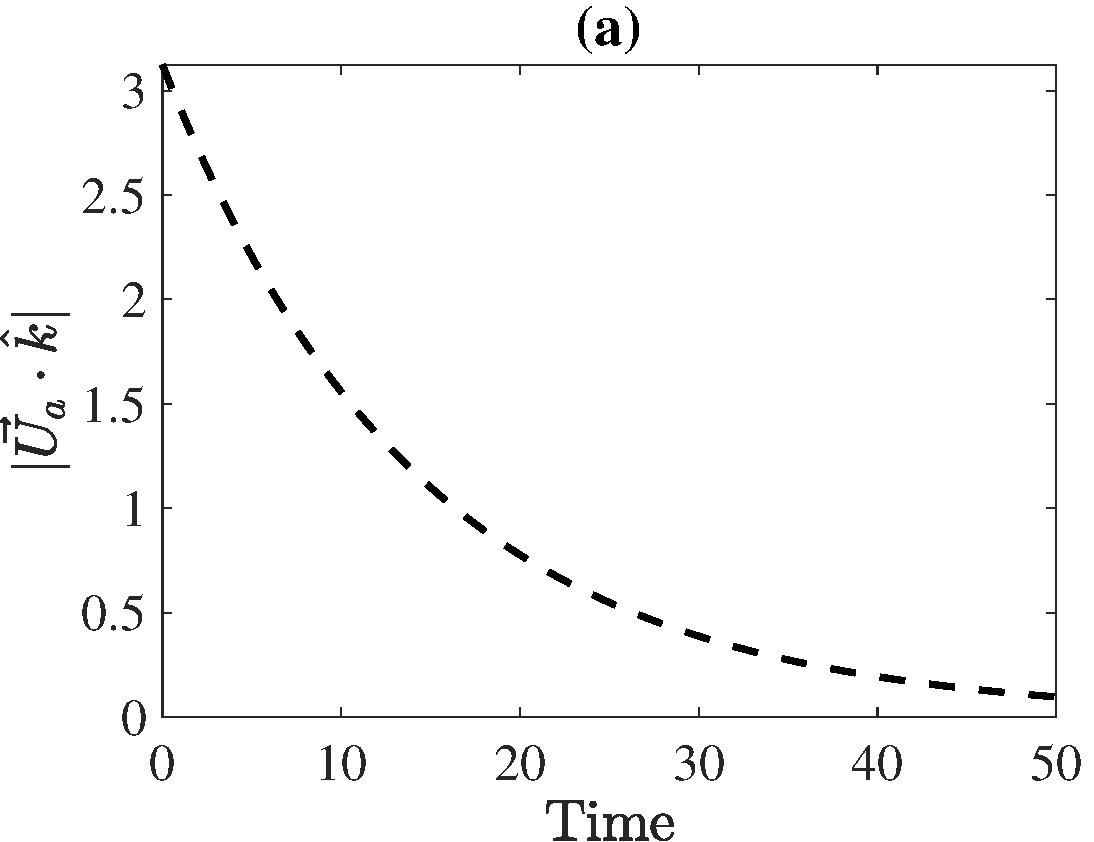
\includegraphics[scale=0.35]{./figures/fig_NC50_bs_Ua3_all.pdf}
		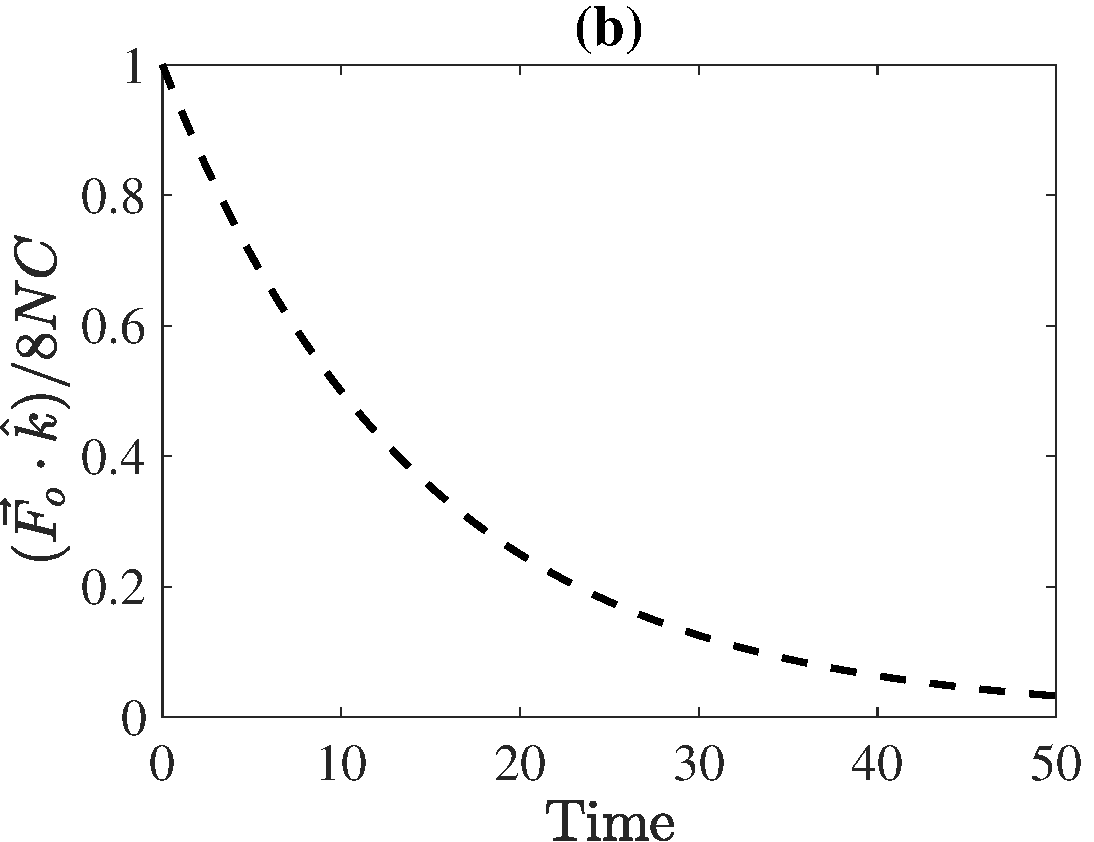
\includegraphics[scale=0.35]{./figures/fig_NC50_bs_Fo3_all}
		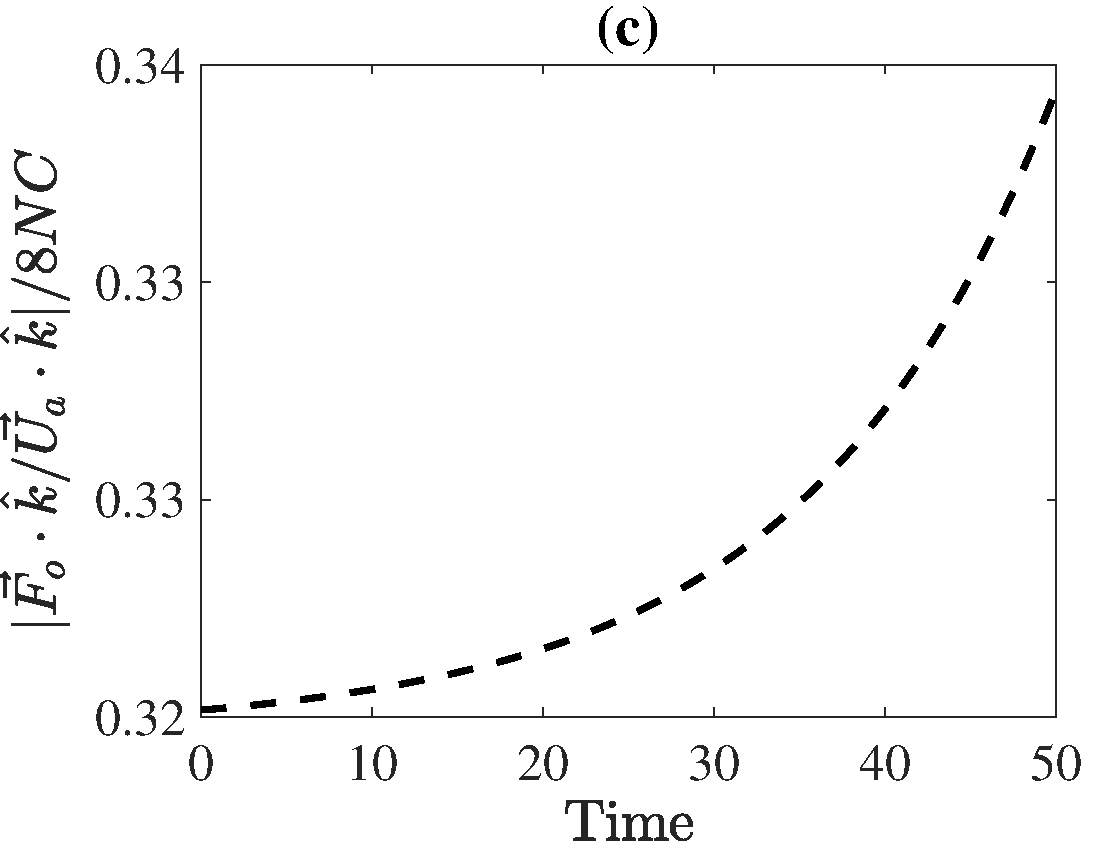
\includegraphics[scale=0.35]{./figures/fig_NC50_bs_Fo3Ua_ratio}
		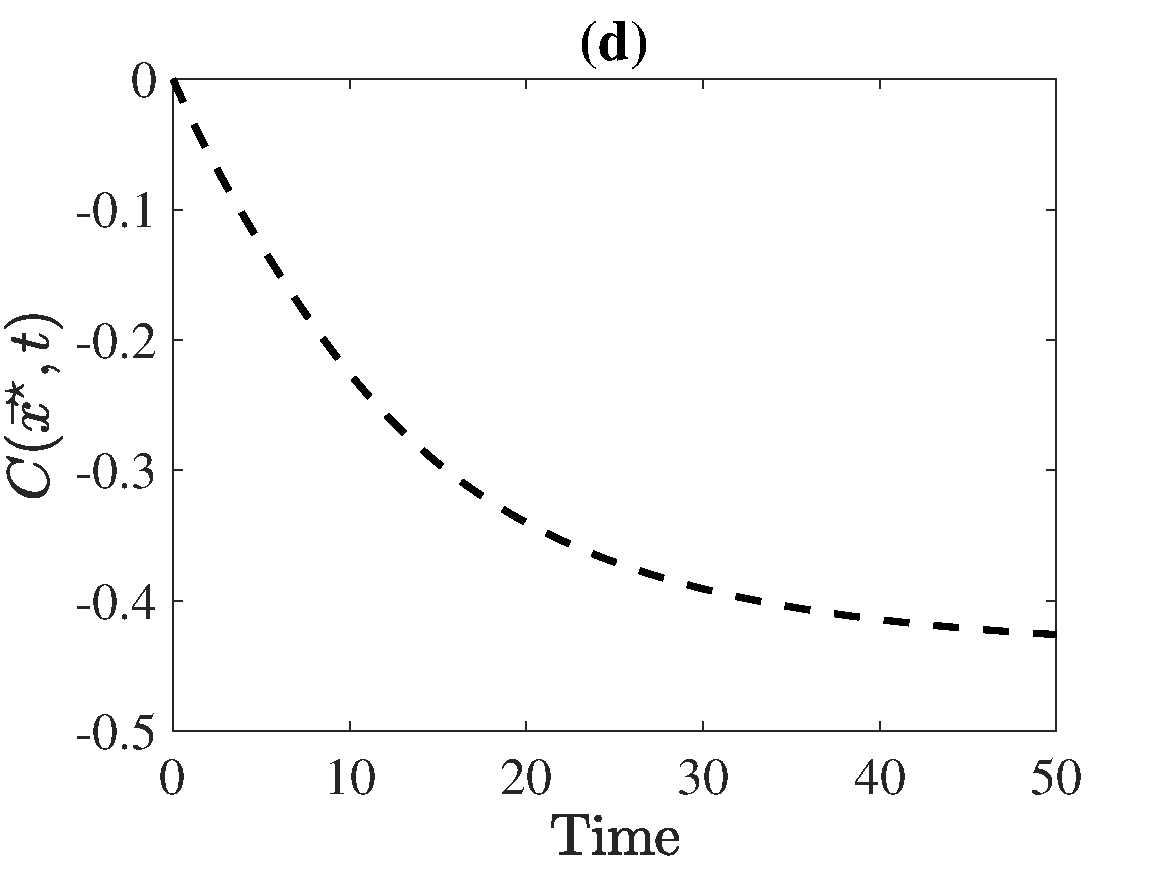
\includegraphics[scale=0.35]{./figures/fig_NC50_bs_C_star}
	\caption{Comparison of various Péclet numbers. We show (a) the settling speed, (b) the vertical component of normalized drag force on the aggregate, (c) the ratio of (b) to (a) values, and (d) the perturbation at position $\vec{x}^{\star}$. }
	\label{fig_NC50_base_case_all}
\end{center}
\end{figure}
\par 
In Figure~\ref{fig_NC50_snaps_all}, we show several 2D snapshots, sliced in the middle of the domain ($x = -0.74$), of the perturbation $C$ at various times. Note that we see negative values of $C$ since the perturbation is a concentration difference from the initial concentration. 
We can observe much higher perturbations around the aggregate that increases in magnitude as time increases as the aggregate entrains upper-layer solute. 
\par
We observe the aggregate behavior more closely in Figure~\ref{fig_NC50_base_case_all}. As we introduced in the previous section, we measure (a) the settling speed and (b) the normalized total drag of the aggregate. We also exhibit the ratio of total drag to the settling speed in plot (c) as a measure of the coefficient in the linear relationship between drag and velocity
that is observed in Stokes flow. Although both settling speed and drag seem to be decreasing over time, we find that their ratio (c) increases non-linearly. This implies that the stratification of the fluid plays a role in the aggregate's settling behavior, not only by reducing the buoyancy but also through the entrained fluid. 
We would have observed a horizontal line if the surrounding fluid did not affect aggregate motion as it settles in a homogeneous fluid. 
\par
In the last plot (d), we observe the perturbation at a particular location outside the aggregate boundary. It is the white star point $\vec{x}^{\star} = (-0.74, 12.74, 0.24)$ in Figure~\ref{fig_NC50_snaps_all}. This point is approximately (1.01 + $R_m$) away from the center of mass of the aggregate. The perturbation is expected to grow in magnitude over time at this point. As the settling motion slows down, the magnitude of perturbation also smoothes out. 
\par
In the next section, we explore various shapes of aggregates made with 50 cubes, in addition to the base case. Afterward, we will observe the effects of varying Péclet numbers and background fluid density stratification $\gamma$. 
\begin{figure}[ht]
	\begin{center}
		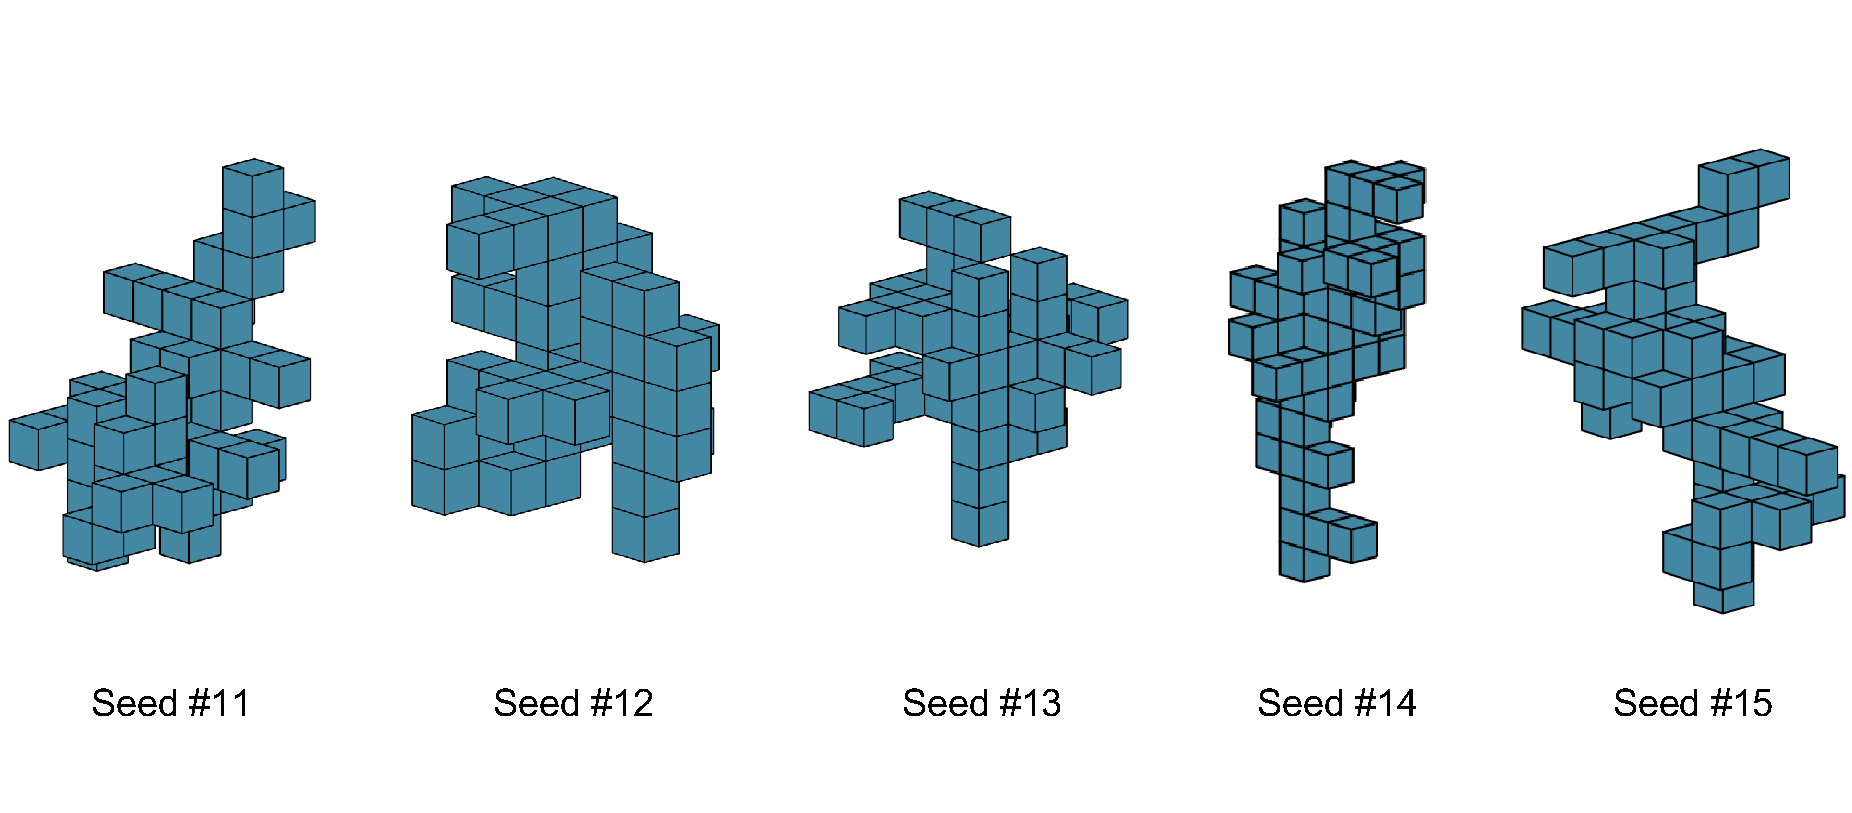
\includegraphics[scale=0.45]{./figures/fig_seed11_15_all.pdf}
	\caption{Five sample aggregates composed of 50 cubes.}
	\label{fig_seed11_15_all}
\end{center}
\end{figure}
\par
\subsection{Various shapes of aggregates}
We first run simulations with randomly shaped aggregates using 50 cubes, in addition to the base case model that is the random seed \#2. We create five more different aggregates, numbering seeds from \#11 to \#15. See Figure~\ref{fig_seed11_15_all}.
With these six sample aggregates, we examine their behaviors. Results are presented in Figure~\ref{fig_NC50_Seeds}.
\begin{figure}[ht]
	\begin{center}
		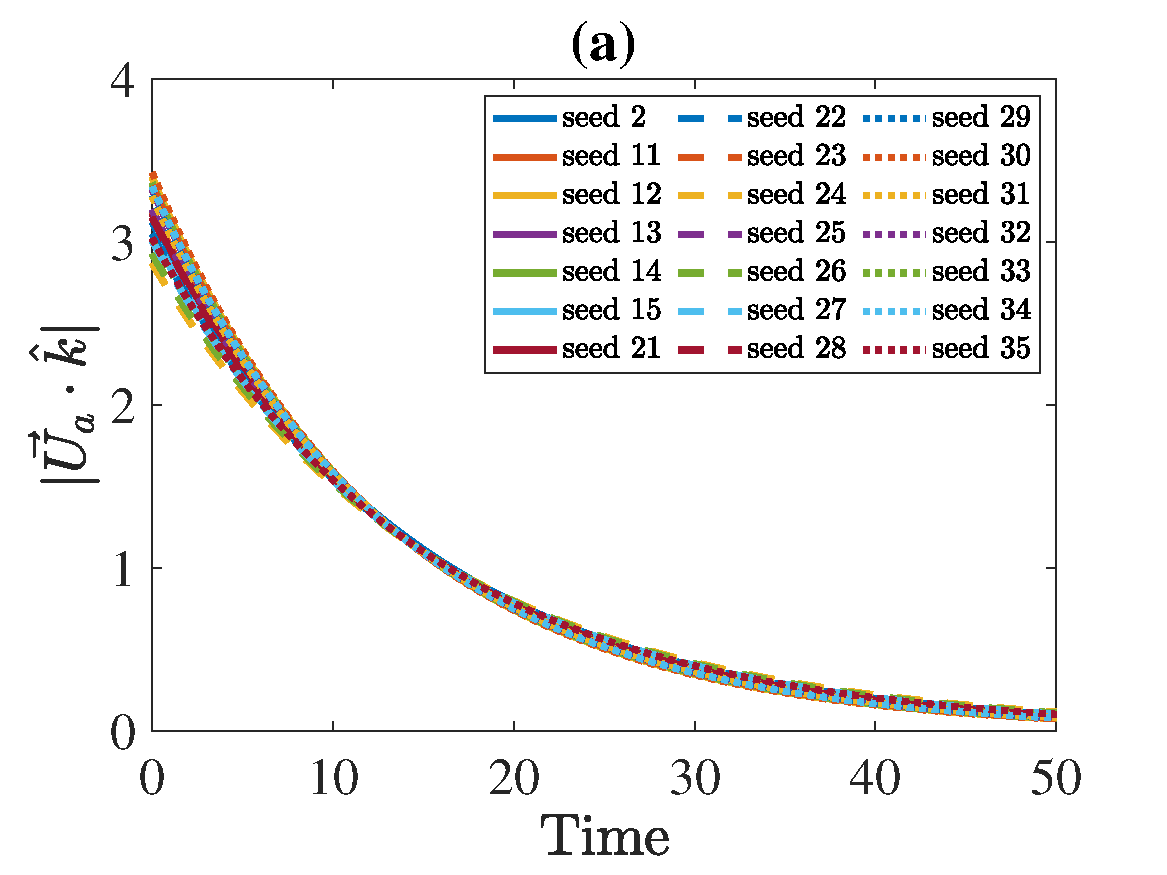
\includegraphics[scale=0.29]{./figures/fig_NC50_sd_Ua3_all}
		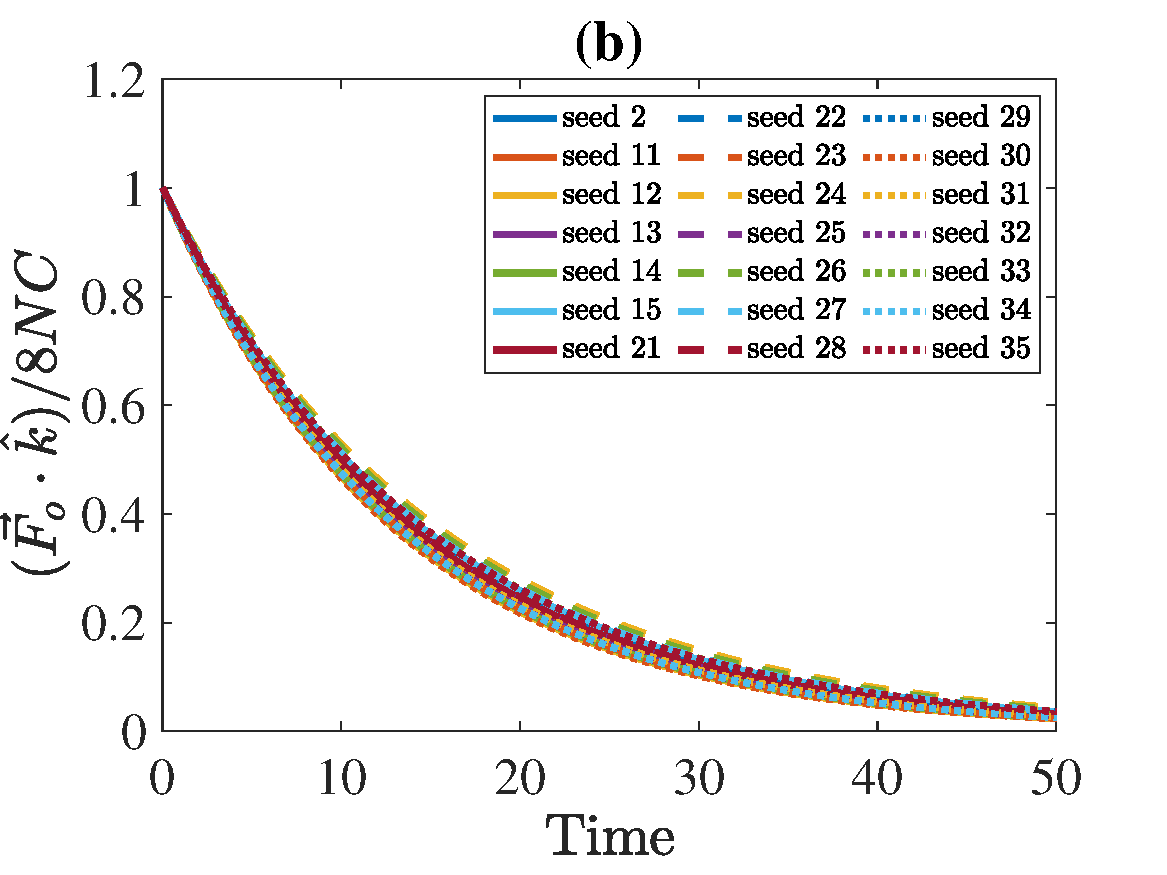
\includegraphics[scale=0.29]{./figures/fig_NC50_sd_Fo3_all}
		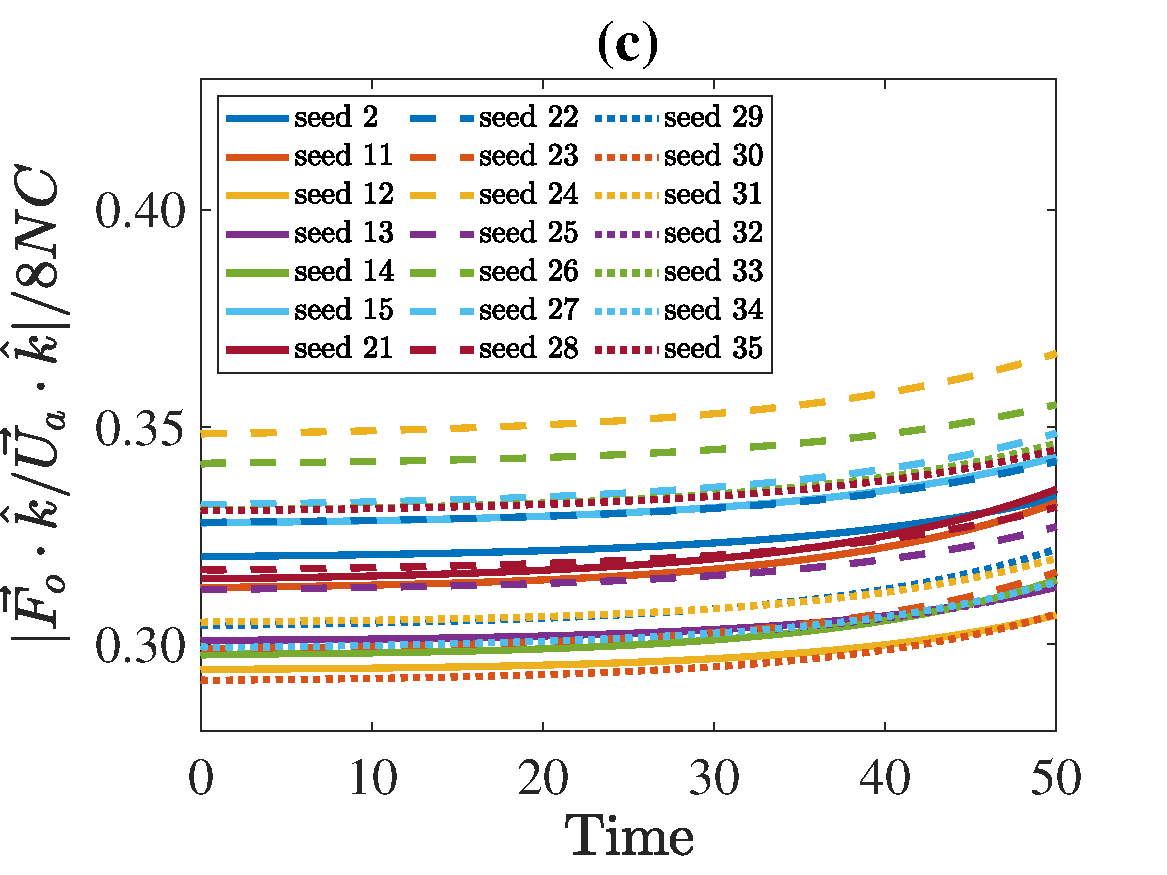
\includegraphics[scale=0.29]{./figures/fig_NC50_sd_Fo3Ua_ratio}
		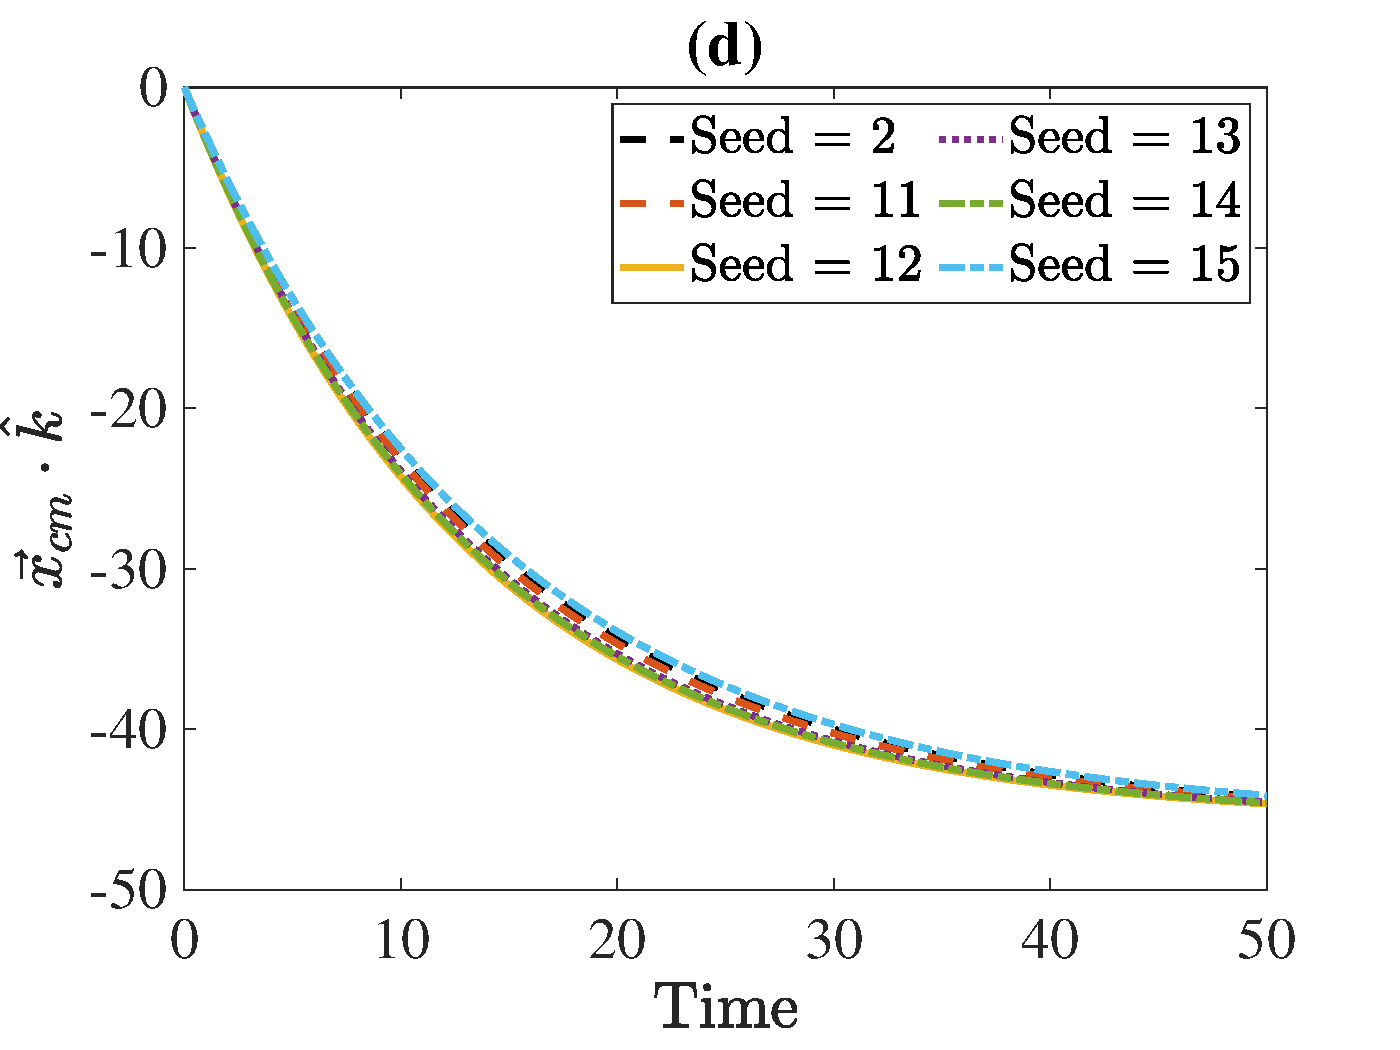
\includegraphics[scale=0.29]{./figures/fig_NC50_sd_cm3_all}
	\caption{Comparison of various shapes of aggregates made with 50 cubes. We show their (a) settling speed, (b) drag force on the aggregate in the settling direction, (c) ratio of (b) to (a) values, and (d) position of the center of mass.}
	\label{fig_NC50_Seeds}
\end{center}
\end{figure}
\par
% When we analyzed the drag forces in a homogeneous fluid in Chapter~\ref{sec:results_translationflow}, we observed the drag distribution of about 15\% with aggregates made with 50 cubes; see Figure~\ref{fig_drag_raw}.
There are some variations (less than 16\%) in aggregates settling behaviors, yet their speed, drag, and $\vec{x}_{cm}$ locations seem to have overall similar motions. 
Meanwhile, plot (c) shows larger differences between each aggregate shape. 
We find this interesting feature that the drag-velocity ratio spread shows approximately a 12\% difference range and 5\% away from their mean value (at the final time). 
Note that the sample mean value at the final time $t = 50$ is about 0.3241.
This demonstrates that modeling an aggregate with a simplified shape, such as a sphere, cannot accurately capture all physical forces involved.
\par
Based on this mean value of six samples, we can estimate the number of random seeds, $N_{sd}$, we should simulate to obtain a finer result. In particular, we want to get the $N_{sd}$ such that the relative error between the standard error ($SE$) and standard error of the mean ($SEM$) is 1\%, i.e.,
\begin{equation}
	\frac{|SE \ - \ SEM|}{SE} < 1 (\%).	
\end{equation}

In our case, we have
\begin{equation}
	SE \ = \frac{\text{Standard deviation with all  } N_{sd}}{\sqrt{N_{sd}}}
\end{equation}
and
\begin{equation}
	SEM \ = \frac{\text{Standard deviation of 6 samples}}{\sqrt{6}}.
\end{equation}
However, since we do not know the numerator of $SE$, we assume that it is the same as the sample standard deviation. We then can solve for $N_{sd} \geq 37$. In the future, we plan to run simulations with $N_{sd}$ many different randomly formed aggregates. 

\subsection{Various Péclet number, Pe}
Next, we vary Péclet numbers; Pe $=1$ and $ 10$ comparing the simulations to the base case for which Pe = 100.  As a smaller Péclet number 
implies more diffusive effects, we look for differences in perturbation. 
Since we have more numerical instability for lower Péclet numbers, we reduce the time step size to $\Delta t = 0.1$ for all three Péclet number cases.
\begin{figure}[ht]
	\begin{center}
		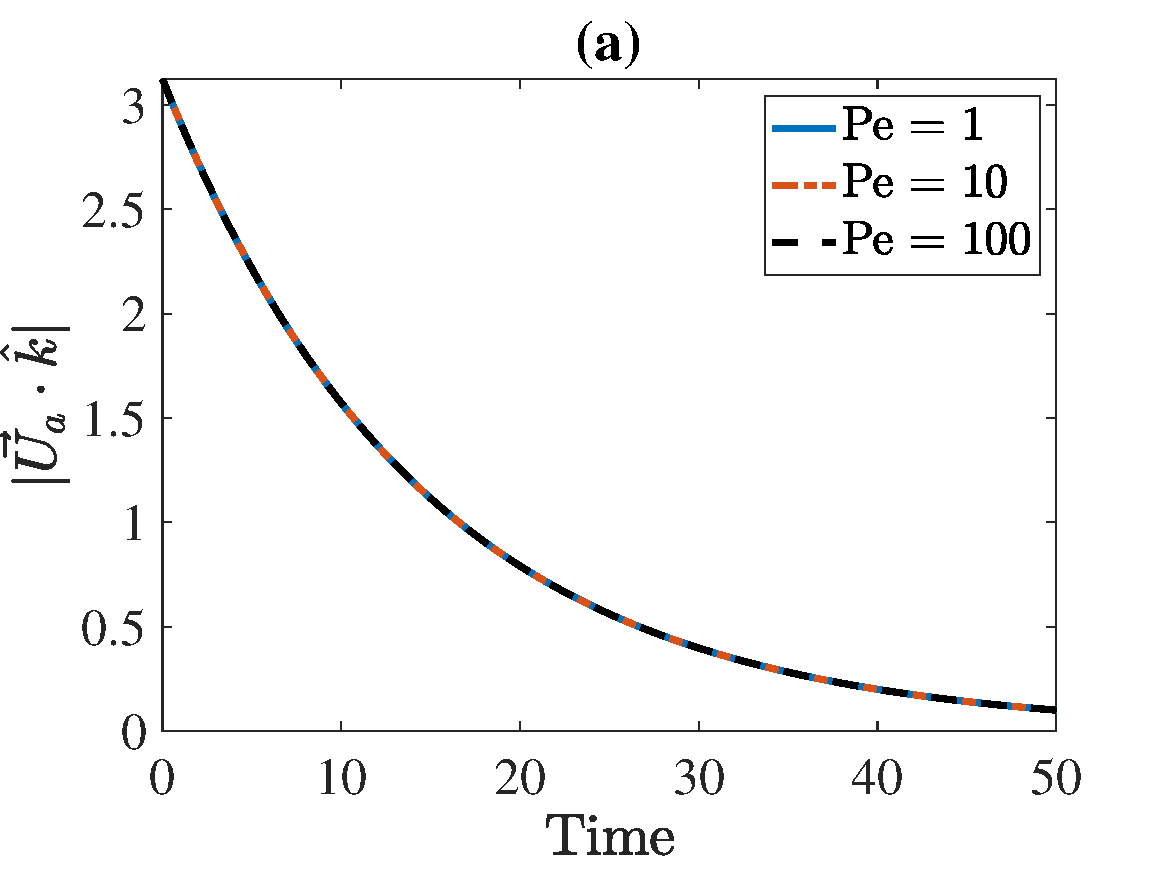
\includegraphics[scale=0.35]{./figures/fig_NC50_Pe_Ua3_all}
		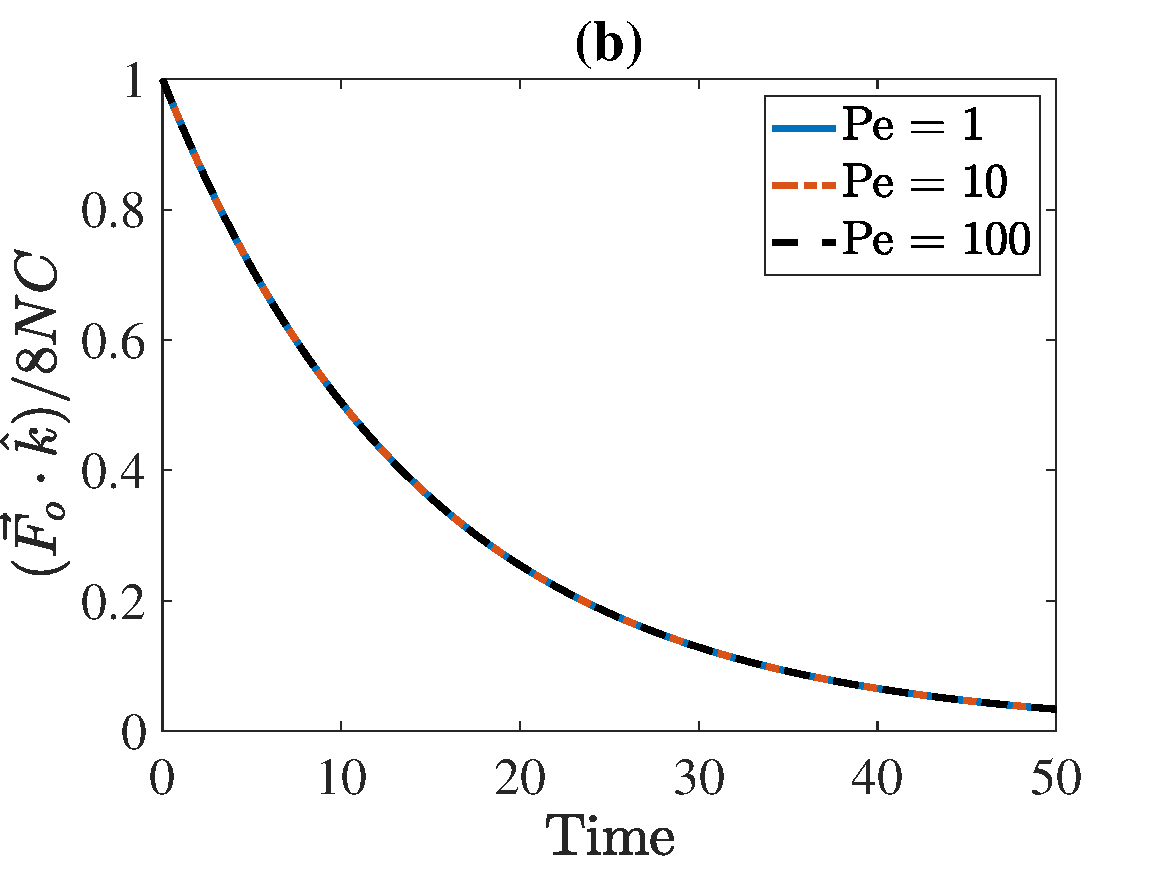
\includegraphics[scale=0.35]{./figures/fig_NC50_Pe_Fo3_all}
		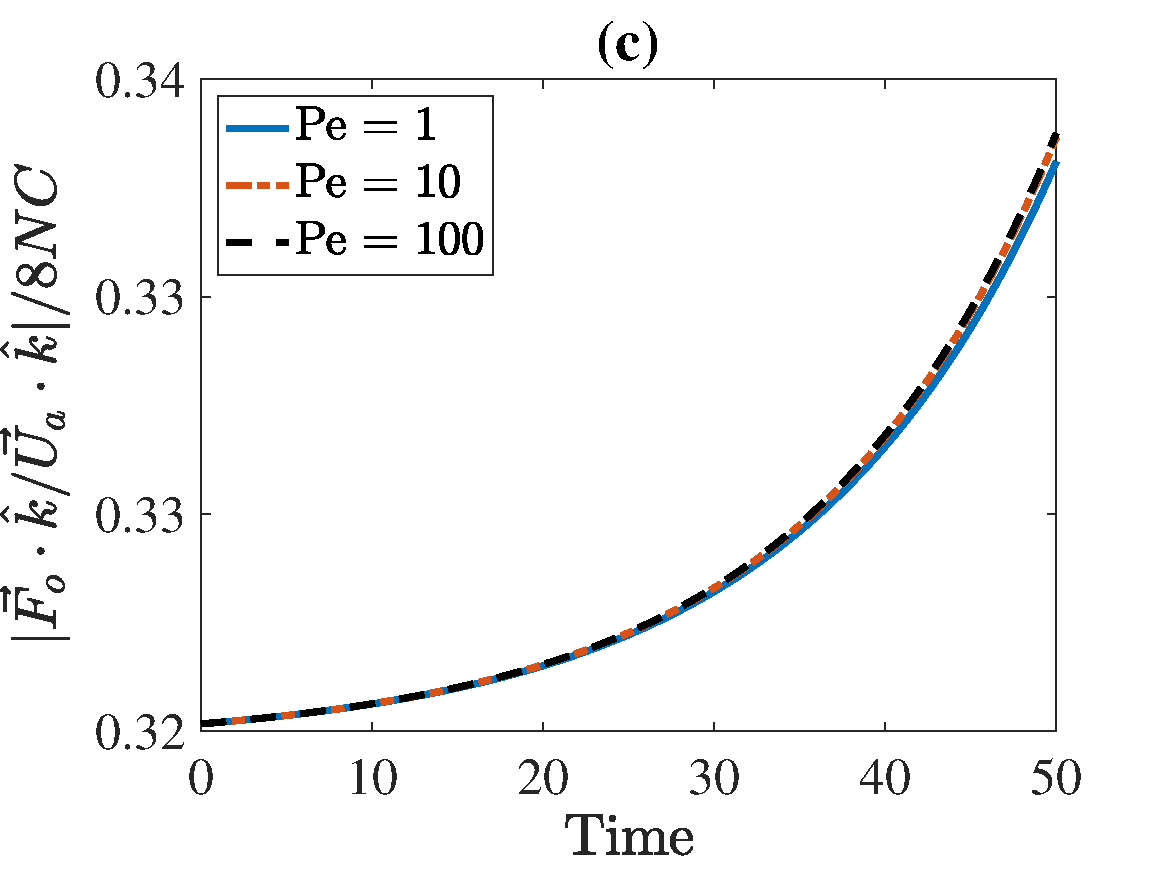
\includegraphics[scale=0.35]{./figures/fig_NC50_Pe_Fo3Ua_ratio}
		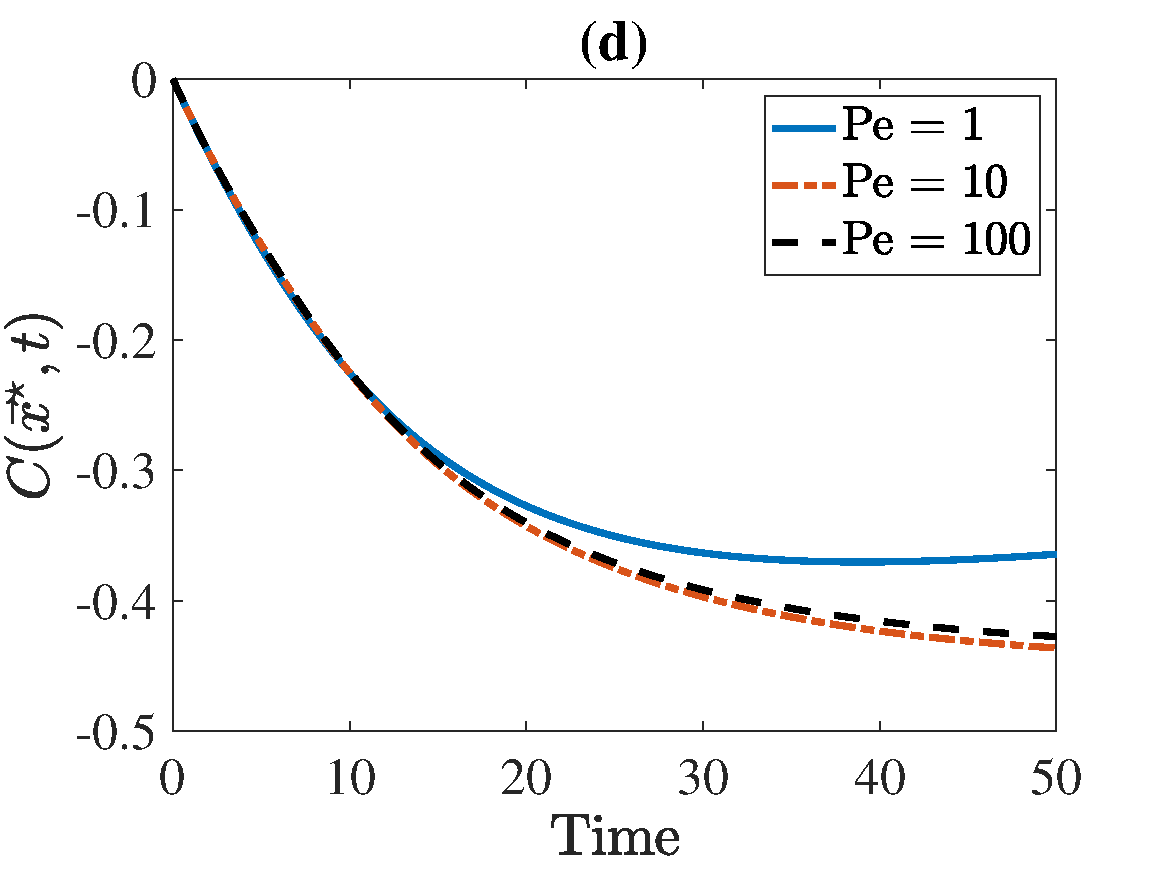
\includegraphics[scale=0.35]{./figures/fig_NC50_Pe_C_star}
	\caption{Comparison of various Péclet numbers. We show (a) the settling speed, (b) the vertical force on the aggregate, (c) the ratio of (b) to (a) values, and (d) the value of the perturbation near the aggregate.}
	\label{fig_NC50_Pe}
\end{center}
\end{figure}
\par
Figure~\ref{fig_NC50_Pe} shows no drastic variations between all three Péclet numbers, especially for the velocity and total drag. 
Focusing on the perturbation plot (d), we can see that more diffusion occurs for the smallest Péclet, Pe = 1, having steady perturbation value after time $t = 30$.
Overall, it is clear that all four plots agree well with our expectations, even though the impact of varying the Péclet number is small in this regime. 
\subsection{Various stratification strength $\gamma$}
Lastly, we investigate three different stratification strengths, 
\[
\gamma = 10^{-4} \times \left[ \ 1, \ 4 \ \text{(base case)}, \  6 \right].
\]
We anticipate observing variations in both aggregate and fluid dynamics as we change the $\gamma$ value. Note that every other parameter is the same as in the base case. 
\begin{figure}[h]
	\begin{center}
		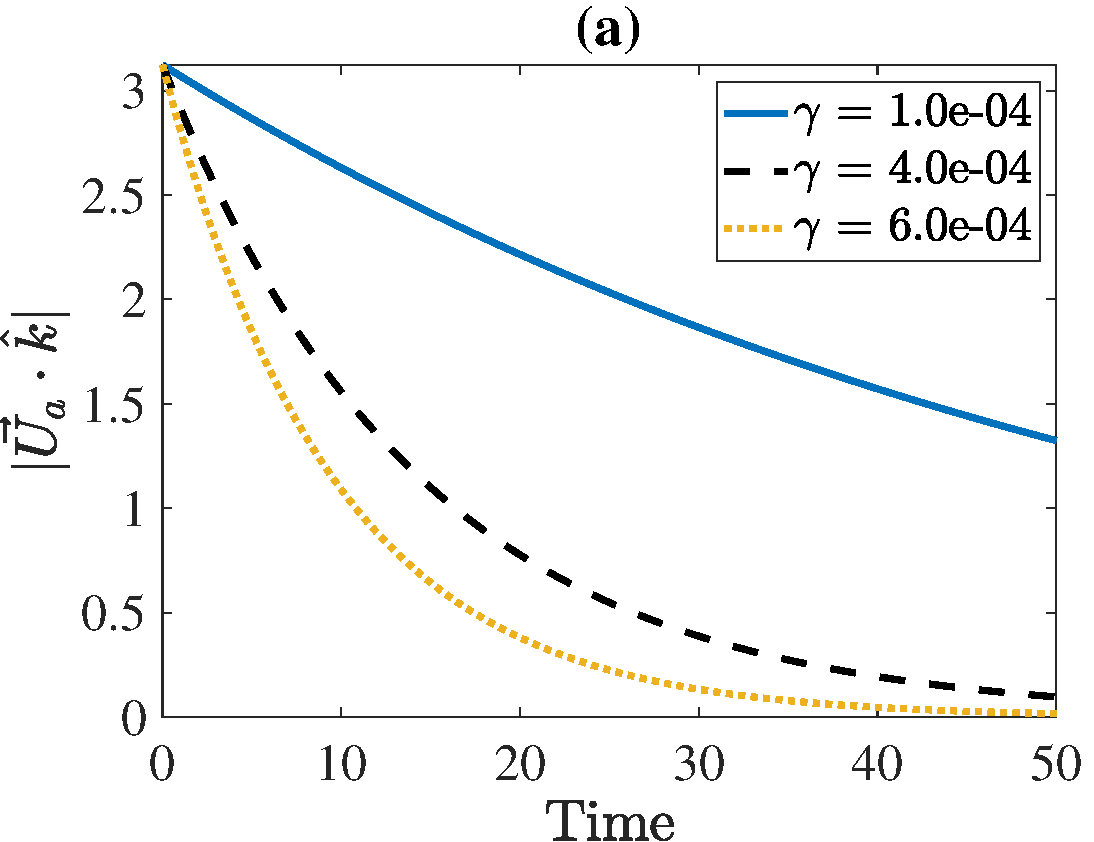
\includegraphics[scale=0.35]{./figures/fig_NC50_g_Ua3_all}
		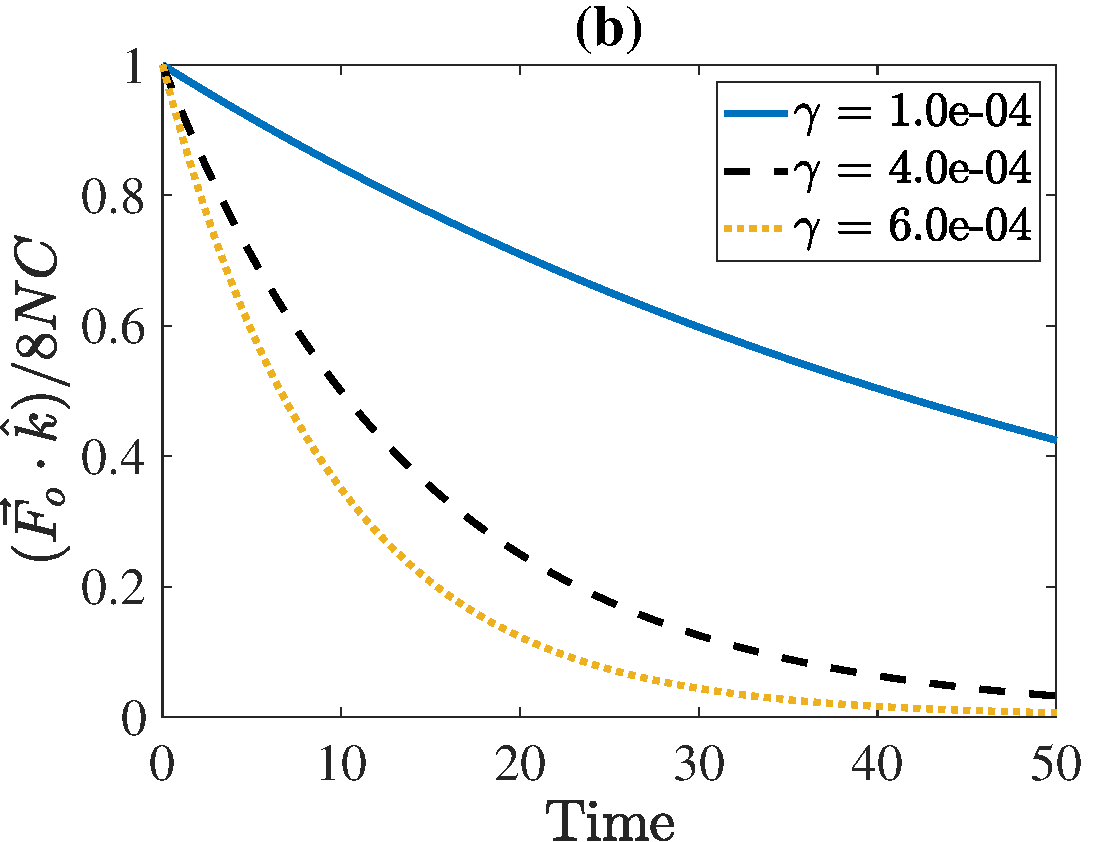
\includegraphics[scale=0.35]{./figures/fig_NC50_g_Fo3_all}
		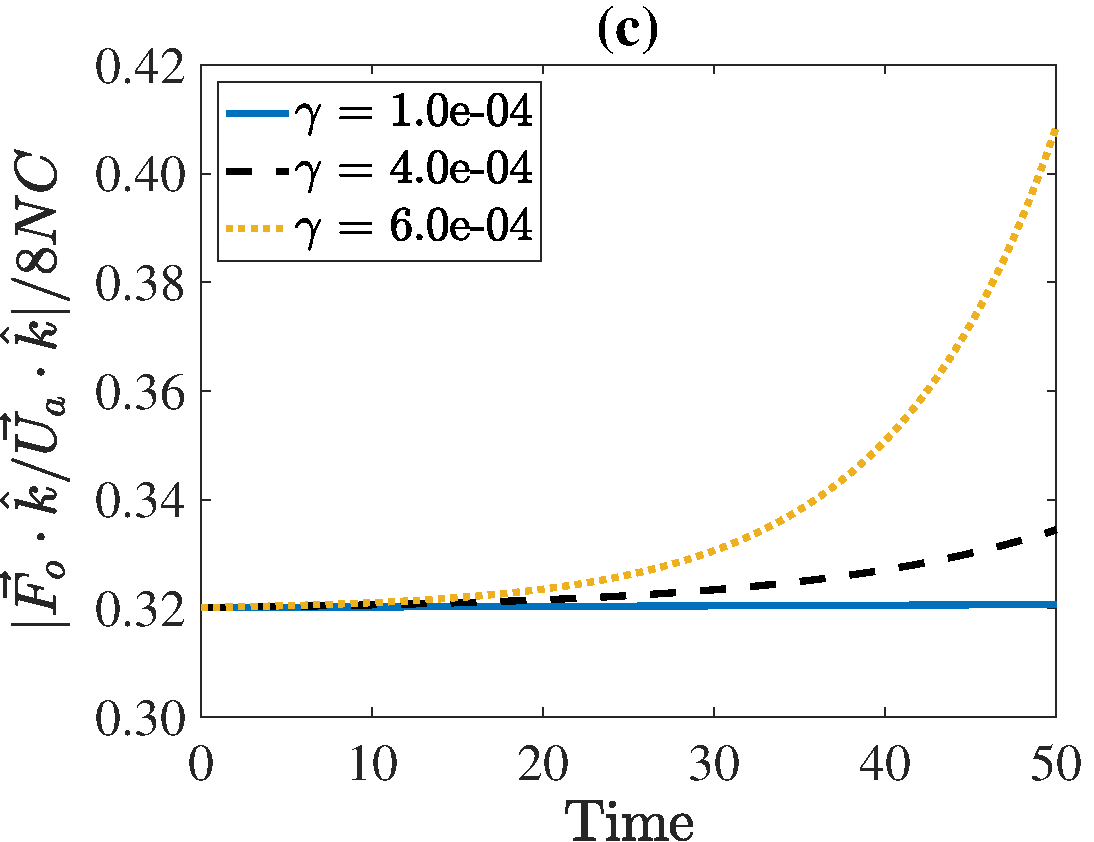
\includegraphics[scale=0.35]{./figures/fig_NC50_g_Fo3Ua_ratio}
		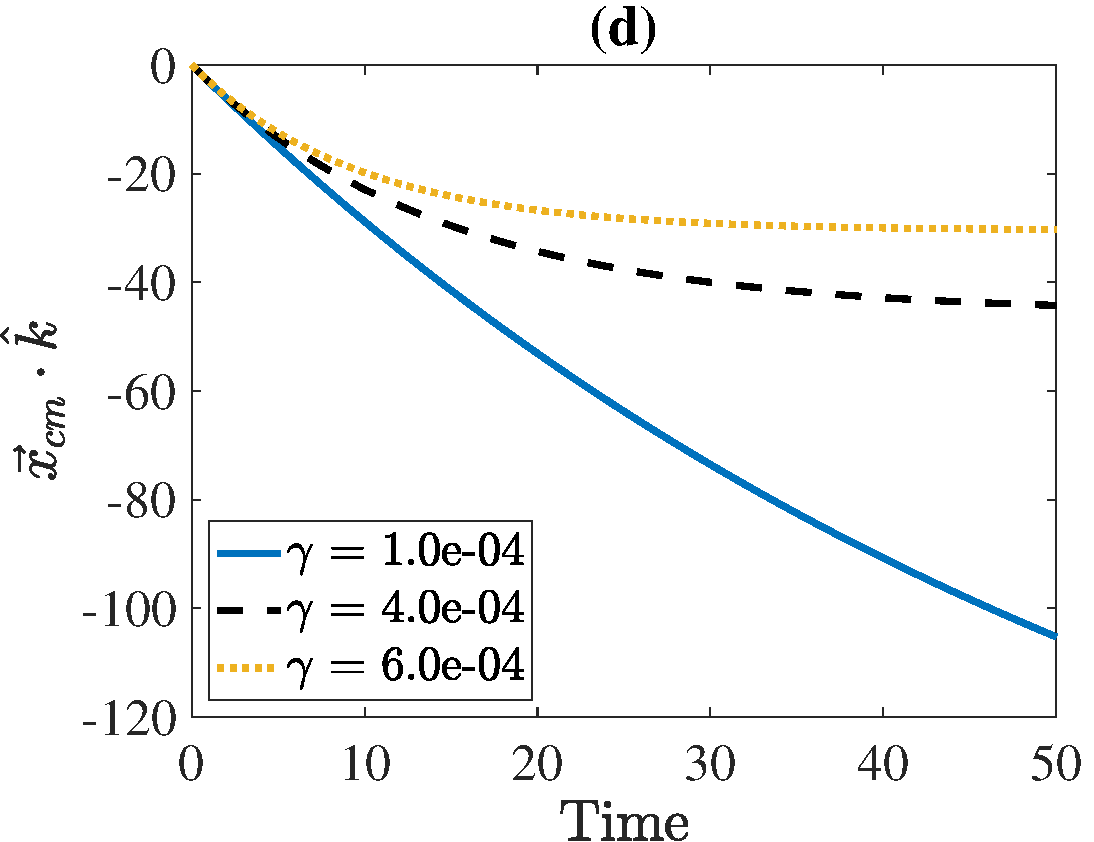
\includegraphics[scale=0.35]{./figures/fig_NC50_g_cm3_all}
	\caption{Comparison of various background density stratification strengths. We show (a) the settling speed, (b) the vertical force on the aggregate, (c) the ratio of (b) to (a) values, and (d) the position of the center of mass }
	\label{fig_NC50_gg}
\end{center}
\end{figure}
\begin{figure}[h]
	\begin{center}
		\includegraphics[scale=0.33]{./figures/fig_NC50_g_C_star.pdf}
		\includegraphics[scale=0.33]{./figures/fig_NC50_g_C_M}
	\caption{Perturbation with various $\gamma$ at (a) the star position $\vec{x}^{\star}$, outside the aggregate, and (b) the center of the fluid domain, inside the aggregate.}
	\label{fig_NC50_gCM}
\end{center}
\end{figure}
\par
We first present quantities of interest 
the aggregate itself in Figure~\ref{fig_NC50_Seeds}. In plot (a), we see that the settling speed of the aggregate decreases faster when the fluid density gradient is sharper. Similar results are shown for the total drag over time in plot (b). To clarify, we present the ratio of the drag to the settling speed in plot (c). We observe very similar behavior as in the homogeneous fluid case with the smallest $\gamma = 10^{-4}$. Note that this $\gamma$ is considered a small value for the aggregate radius $R_a \approx 9$. For instance, the same $\gamma$ may be a large enough value to observe a clear background fluid stratification effect for an aggregate radius 20.
We also look at the center of mass of aggregate over time. Since $\gamma = 10^{-4}$ mimics a homogeneous fluid, the aggregate travels more, yet with a slower speed, demonstrated by the blue solid line in plot (d).
\par
From a fluid perspective, we obtain the perturbation over time at two different points. In Figure~\ref{fig_NC50_gCM}, the left plot is the perturbation at the usual point, $\vec{x}^{\star}$, where the white star is located in Figure~\ref{fig_NC50_snaps_all}. It is located outside of the aggregate, yet very close. On the right side, we examine the perturbation inside of the aggregate, particularly at the center of the fluid domain. By looking at the magnitude of $C$, there are certainly higher perturbations for all three $\gamma$ cases at $\vec{x}_m$. Moreover, the perturbation varying range is quite large for the light stratification case (blue line). As we mentioned, it is because the same aggregate stops moving in a stronger density-stratified fluid due to reaching neutral buoyancy.
\section{Conclusion}
As an extension of our study of the homogeneous system~\cite{yoo_hydrodynamic_2020}, we have developed a numerical method to simulate a settling marine aggregate, randomly formed with cubes, using a boundary integral method in a density-stratified fluid.
Applying the net force equilibrium in a Stokes regime, we prescribed the total drag and torque to solve for the stress on the aggregate and its settling velocity using the single-layer potential formula.
With the velocity field obtained, we advance the perturbation in time using the advection-diffusion equation. 
To accelerate the evaluation of integrals of Stokeslet, we incorporate the Fast Multipole Method by modifying the Laplace kernel.
\par
We have validated our methods by providing results of a settling aggregate composed of 10 cubes while varying the spatial grid, time steps, and domain sizes. 
Most of the errors for each comparison appeared to be much smaller than those resulting from assuming that the stress is uniform on each square face of a cube.
\par
Furthermore, we simulated larger aggregates, made with 50 cubes, in different settings. We have observed aggregate settling behavior before its density matches the surrounding fluid density.
We found a consistent trend in the settling behaviors between different shapes of aggregates with, for example, variations in the drag coefficient of the order of 8\%.   
In future work, we can simulate aggregates with more cubes and consider more different shapes for better statistical results. kk
Under the different Péclet number environments, we find the main changes in the perturbation, as expected, between Pe = 1 and Pe = 10. Since a smaller Péclet number implies a higher diffusivity, the perturbation near the aggregate slows down 10\% faster than the other two cases. 
\par
We also explore various stratification strengths via $\gamma$ values. 
Marine aggregates are highly porous and sensitive to surrounding fluid density stratification~\cite{prairie_delayed_2013}. Our results also support these characteristics while we perform the simulations with three types of background fluid density gradients.
In addition to our results in this thesis, potential future work includes considering another applicable regime with different parameters.
\par
We note that a description of rotational flow results is missing, although we have allowed a rotation of an aggregate while obtaining all the numerical results. In short, we have found an approximate torque having the order $\mathcal{O}(10^{-4})$. This is quite a small value compared to the drag force and perturbation effects as a response to the background fluid stratification. 
We consider analyzing more details as future work.
\par
There are several branches we can extend our research further with our comprehensive numerical tools developed. As much research work has been done with a sphere model as an aggregate, we would like to compare our results, such as the settling speed, drag acting on the aggregate, and the amount of concentration entrained. 


 

\chapter{Continuum modeling of a complex fluid}
\label{ch:4}
\par
In this chapter, I report the summer 2023 internship work at LBNL and additional numerical implementations I continued to finish this thesis.

As we mentioned in Chapter \ref{sec:intro_complex_fluid}, we consider the deviatoric stress tensor of the form as in equation (\ref{eq_CN_tau}), 
\begin{equation}
  \boldsymbol{\tau} =
  \nu_0  \bm{A}_1 +  \nu_1  \bm{A}_1^2 + \nu_2 \bm{A}_2 ,
\nonumber
\end{equation}
where each $\nu_i$ for $i = 0,1,2$ is dependent on the materials or flow types. In this project, we explore two examples: 1) granular materials and 2) non-colloidal suspension in a Newtonian fluid. While the big picture of a viscous term is the same as described in equation (\ref{eq_CN_tau}), the way to obtain the coefficients $\nu_i$ are different. We thus address establishing the viscosity terms first for both examples. Then, we examine each flow in geometry by solving the Navier-Stokes equation,
in which they were introduced in Chapter 1; equations (\ref{eq_conserv_mass}) and (\ref{eq_momentum_NS}).
\par
In the AMReX-incflo code, we can only use the explicit Euler time integration method due to the stress tensor $\bm{\tau}$ having a quadratic relationship with the strain rate $\bm{D}$, which is a function of the velocity $\vec{u}$. 
To clarify, we write the tensor $\bm{\tau}$ in terms of $\bm{D}$ explicitly,
\begin{equation}
  \boldsymbol{\tau} =
  2 \nu_0  \bm{D} +  2 \nu_1  \bm{D}^2 
  + 2\nu_2 \left(
    \frac{\partial \bm{D}}{\partial t} + 
     \vec{u} \cdot \nabla \bm{D}
    +\bm{D} \nabla \vec{u}+ \left(\nabla \vec{u} \right)^T \bm{D} 
   \right)
\end{equation}
% Let's look at the last term a little more closely:
% \begin{equation}
%   \nu_2 \left(
%    \frac{\partial }{\partial t}\left( \nabla \vec{u} +  \nabla\vec{u}^T \right) + 
%     \vec{u} \cdot \nabla \left(  \nabla\vec{u} +  \nabla\vec{u}^T \right) 
%    +\left(  \nabla\vec{u} + \nabla \vec{u}^T \right)  \nabla \vec{u}+ \left(\nabla \vec{u} \right)^T \left(  \nabla\vec{u} +  \nabla\vec{u}^T \right) 
%   \right)
% \end{equation}
% \begin{equation}
%   \nu_2 \left(
%    2\frac{\partial \bm{D} }{\partial t}
%    + \left(\nabla\vec{u}  \right)^2
%   + 2(\nabla \vec{u})^T  \nabla \vec{u}+
%    \left(    \nabla\vec{u}^T \right)^2
%   \right)
% \end{equation}
To achieve second-order convergence, we implement two more time integration methods in incflo. As a simpler step, we coded the explicit Runge-Kutta 2 (RK2) scheme. We then attempt to use a predictor-corrector method, which is a fully implicit formula.
\par
The order of this chapter is the following. We explain the computation of viscosities for granular materials and non-colloidal suspension in a Newtonian fluid. Then, we discuss the numerical methods,   Then,  We close this chapter by showing some numerical results.

\section{Granular rheology}
Depending on the level of stress, viscoplastic fluids either flow or act like rigid solids. The minimum value that makes viscoplastic fluids move is called yield stress. 
We can easily find viscoplastic materials in our lives; for example, toothpaste, and whipped cream. 
Among many different types, we particularly study those granular materials. They are also considered viscoplastic fluids, depending on the states. For instance, a medicine tablet (pill) is considered a solid. However, the powder of ingredients acts as a fluid since it flows. 
There are many factors we need to learn to have a full understanding of granular materials' behavior.
Since the yield stress is the main value to understand different phases (liquid vs solid) of continuum granular flow, we focus on computing more accurate stress, by taking pressure into account. The source of pressure can be friction between granular matters or external forces.  
We consider both the shear stress rate and the pressure onto the granular materials as the sources of yield stress. 
\par
In Chapter 1, we introduced the stress tensor for the fluid momentum equation in equation (\ref{eq_stress_tensor}). 
We now express a new stress tensor $\bm \tau$ with a higher-order strain rate that can describe non-isotropic (meaning material properties changes along with direction) flow effects,
\begin{align}
  \bar{\bar{\sigma}}
    = -P \bar{\bar{I}}  + \bm{\tau}
    =  -P \bar{\bar{I}}  
    + \mu_1(\dot{\gamma}) \mathcal{O}({\bm D})
    + \mu_2(\dot{\gamma}) \mathcal{O}({\bm D^2}).
  \end{align}
In this section, we focus on the methodology to compute the viscosity $\mu_i ({\dot{\gamma}})$ ($i = 1,2$) under the simple shear flow. 
% A new apparent viscosity computation using the well-known $\mu(I)$ relation can also be found [{\color{blue}REFERENCE}]. 


To describe a non-isotropic flow, we consider the deviatoric stress tensor of the form (\ref{eq_2ndOrder_tau}), which is derived under two conditions:
(1) the flow motion is simple with a constant stretch history by neglecting deformation history, and (2) the flow is isochoric, having uniform properties along streamlines and tr$(D) = 0$. 
In particular, we see \cite{srivastava_viscometric_2021}
% \begin{align*}
% \bar{\bar{\sigma}} - P {\bm I} \equiv
%   {\bm {\bm \tau}}
%   =  \ \mu_1 {\bm D} 
%   + \mu_2  \left[ {\bm D}^2  - \frac{\text{tr}\left({\bm D}^2\right)}{3}{\bm I} \right]
%   + \eta_3  \left[ {\bm D}{\bm W} - {\bm W}{\bm D} \right]
%   \nonumber \\
%   + \frac{\kappa_1}{\dot{\gamma }^2} \bm D 
%   + \frac{\kappa_2}{\dot{\gamma }^2}  \left[ {\bm D}^2  
%   - \frac{\text{tr}\left({\bm D}^2\right)}{3}{\bm I} \right],
% \end{align*}
\begin{equation}
  {\bm {\bm \tau}}
  = \mu_1(\dot{\gamma}) {\bm D}
  \ +  \ 
 \mu_2 (\dot{\gamma})
  \left[ {\bm D}^2  - \frac{\text{tr}\left({\bm D}^2\right)}{3}{\bm I} \right],
  % \ + \
  % \left( \mu_3 \dot{\gamma}^2 \right)
  % \frac{1}{\dot{\gamma}^2}
  %   \left[ {\bm D}{\bm W} - {\bm W}{\bm D} \right]
\label{eq_2ndOrder_tau}
\end{equation}
where 
\begin{equation}
  \mu_1 (\dot{\gamma})
   = \left( \eta_1 \dot{\gamma}+ \kappa_1 \right) \frac{1}{\dot{\gamma}},
\label{eq_mu1_main}
\end{equation}
and 
\begin{equation}
  \mu_2 (\dot{\gamma}) = 
  \left( \eta_2  \dot{\gamma}^2
  +  \kappa_2 
  \right) \frac{1}{\dot{\gamma}^2}
  \label{eq_mu2_main}
\end{equation}
Note that the magnitude of strain rate, $\dot{\gamma}$, can be computed by applying the scaled Frobenius norm for a second-order tensor, 
\[
  \dot{\gamma}  = |\bm{D}| = \sqrt{\frac{1}{2}
    \text{tr}\left(\bm{D} \bm{D}^{T} \right)}.
\]
In general, the Frobenius norm states $\bm{D}^H$ instead of $\bm{D}^T$. Since we consider real-valued tensors, it is valid to have $\bm{D}^H = \bm{D}^T$.
\par
We also note that the functions, $\eta_i$ and $\kappa_i$ for $i = 1,2$, have the following dependency to the total stress: each $\eta_i(\dot{\gamma}, p)$ is (shear) rate-dependent and $\kappa_i (p)$ is (shear) rate-independent. 
Along with the shear effect from $\eta_1$, we can observe the second normal-stress difference in shear flows from $\eta_2$.
The rate-independent terms, $\kappa_1$ and $\kappa_2$, allow us to find yield stress. 
We explain the details of these two types of functions in the following sub-section.

\subsection{$\mu (I)$ rheology}
The main key to getting $\eta_i$ and $\kappa_i$ terms is the well-known $\mu(I)$ relationship developed by \textit{Jop, 2006}~\cite{jop_constitutive_2006}.
Here, $I$ is called the \textit{inertial number} defined as 
\begin{equation}
  I =  \frac{\dot{\gamma} d }{\sqrt{P/\rho_p}},
  \label{eq_inertialI}
\end{equation}
where $d$ and $\rho_p$ are the average particle diameter and density of given granular material.
This dimensionless quantity describes the average static force compared to the inertial force between granular particles. Jop, in~\cite{jop_constitutive_2006}, interpreted the inertial number as the ratio between a macroscopic deformation and an inertial timescale. 
\par
We bring an hourglass example to describe the granular flow regimes depending on the inertial number. 
\begin{figure}[ht]
  \begin{center}
    \includegraphics[scale=0.2]{figures/fig_hourglass.pdf}
    \end{center}
  \caption{Schematics of granular flow with an hourglass example.}
  \label{fig_hourglass}
\end{figure}
As we can see in Figure~\ref{fig_hourglass}, three different states can co-exist in granular materials. 
When we look at the top part of the hourglass, filled with sand, it typically seems not to move and resembles a solid. 
As we move our sight toward the middle nozzle of the hourglass, we can observe the sands passing through the nozzle, flowing like a liquid.
Meanwhile, the sand landing on the bottom part of the hourglass is forming a cone shape. When we look very closely at the top of the cone, we can see that the sand is falling and colliding, i.e., it behaves like a gas.
\par
In general, these three regimes can be categorized by the inertial number $I$. The solid-like status appears when $I$ is small. As the number $I$ increases, the flow deformation occurs rapidly, as we see in the middle of the hourglass. Naturally, the collisional flow can be observed for a large $I$ number. 
\par
By applying this $\mu(I)$ rheology, Srivastava~\cite{srivastava_viscometric_2021} devleoped a callibration to obtain the coefficients $\eta_i$ and $\kappa_i$.
For the first-order strain rate viscosity term, equation (\ref{eq_mu1_main}), we have 
\begin{equation}
  \mu_1(I) = \mu_1^0 + A_1{ I}^{ \alpha_1} =  \frac{(\eta_1 \dot{\gamma} + \kappa_1)}{P},\
\label{eq_muI1}
\end{equation}
where $\mu_1^0, A_1,$ and $\alpha_1$ are fitting parameters, depending on matrials. 
By substituting the inertial number $I$, equation (\ref{eq_inertialI}), into equation (\ref{eq_muI1}), we get
\begin{equation}
     \mu_1^0 + A_1 {\left(  \frac{\dot{\gamma} a }{\sqrt{P/\rho}}\right) }^{ \alpha_1} =  \frac{(\eta_1 \dot{\gamma} + \kappa_1)}{P}.
\end{equation}
We then find $\mu_1 (\dot{\gamma}, P)$ and $\kappa_1(p)$ as
\begin{equation}
    \mu_1  (\dot{\gamma}, P)= 
    \biggl( A_1 {\left(   d  \sqrt{\rho} \right) }^{ \alpha_1}\biggr) 
     \dot{\gamma}^{\alpha-1} P^{1-\alpha/2}
\label{eq_eta1}
\end{equation}
\begin{equation}
    \kappa_1(P) = \mu_1^0 P
\label{eq_kappa1}
\end{equation}
\par
Similarly, we can find the coefficients for the quadratic in ${\bm D}$ terms, having the $\mu(I)$ relationship as follows:
\begin{equation}
    \mu_2(I) = \mu_2^0 + A_2{ I^2}^{ \alpha_1} =  \frac{(\eta_2 \dot{\gamma}^2 + \kappa_2)}{P},\
\label{eq_muI2}
\end{equation}
Then, we obtain $\mu_2 (\dot{\gamma}, P)$ and $\kappa_2(P)$
\begin{equation}
    \mu_2  (\dot{\gamma}, P)= 
    \biggl( A_2 {\left(   d  \sqrt{\rho} \right) }^{ 2\alpha_2}\biggr) 
     {\dot{\gamma}}^{2(\alpha_2-1)} P^{1-\alpha_2}
\label{eq_eta2}
\end{equation}
\begin{equation}
    \kappa_2(P) = \mu_2^0 P
\label{eq_kappa2}
\end{equation}

%--------------------------------------------------
We can obtain the flow fitting parameters from particle-based simulations, such as the discrete element method (DEM). The following numbers are introduced in, Jop 2006 \cite{jop_constitutive_2006}; Srivastava 2021 \cite{srivastava_viscometric_2021}:
    \[
    0.09 \leq \mu_1^0 \leq 0.33, 
    \ \ \ \ \ \ \ 
    0.37 \leq \alpha_1 \leq 0.7
    \]
        \[
    0.01 \leq \mu_2^0 \leq 0.1, 
    \ \ \ \ \ \ \ 
    0.28 \leq \alpha_2 \leq 0.44.
    \]
            \[
    \ \ \ \ \ \ \ 
    0.75 \leq \alpha_3 \leq 0.85.
    \]
     One can find the corresponding $A_i$ values in Srivastava 2021 \cite{srivastava_viscometric_2021}.
\subsection{Computation of pressure-dependent apparent viscosity}
For granular rheology, it is typical to see compressible flow. It is, thus, essential to take pressure into account to evaluate viscosity.
Here, we consider the pressure as a combination of background flow pressure, $P_0$, that is linear in the vertical direction, and perturbation, $P'$ such that
\[
P = P_0(y) + P'(x,y,z).\]
Note that we can have the perturbations under gravity. Without gravitational force, we may simply input the constant pressure, $P_0$, and keep it over time.
\par
In case gravity is involved, we consider the density term, in order to approximate the perturbation, as 
\[
\rho  = \rho_0  + \rho'(x,y,z), 
\]
where $\rho_0$ is constant and $\rho'$ is spacial-dependant density perturbation of the flow. 
Here, we assume that 
\begin{equation}
    \nabla P_0  = \frac{d P_0}{d y} \approx \rho_0  g.  
\label{eq_p0_rho0}
\end{equation}
This recovers our momentum equation. As we would like to construct a background pressure that stays over time for our granular rheology, we may use this hidden assumption.
By taking integral both sides of Equation (\ref{eq_p0_rho0}), we obtain
\begin{equation}
    P_0 \approx p_{bg} + \nabla P_0 y.
\end{equation}
We would like to use this form since we already have the $p_{bg}$ term computed in the \verb+incflo+ code (This value is \verb+gp0+).
%
When we have a periodic boundary in the gravity direction, we might need to prescribe a pressure gradient to have an additional pressure effect. 
\par
The main challenge we faced to implement the pressure-dependent viscosity was connecting the pressure in addition to the strain rate into the rheology code. To have physical consistency, we need to solve for a compressible flow model. We thus leave the pressure-dependent granular flow as a future work.
% {\color{blue} Are we keeping this the whole time? Is there any pressure change over time? Does a volume fraction come into play?}

% a little more details
\subsection{Viscosity regularization}
When we evaluate the viscosities, equations (\ref{eq_mu1_main}) and (\ref{eq_mu2_main}), we may encounter a (nearly) singularity as $\dot{\gamma}$ approaches zero.
As AMReX-\verb+incflo+ has the Papanastasiou regularization method implemented, we simply apply the same method for the new granular flow viscosity computations.
\par
By introducing a small parameter, denoted as $\varepsilon$, we can regularize the singularity of $\dot{\gamma}$ as following,
\[
  \frac{1}{\dot{\gamma}} \rightarrow \frac{1-e^{-\dot{\gamma} / \varepsilon}}{\dot{\gamma}}  
\]
for $\dot{\gamma}/\varepsilon \gg 1$. Otherwise, we simply use $1/\varepsilon$. 
The detailed mathematics and analysis can be found in Sverdrup 2018~\cite{sverdrup_highly_2018}.
\section{Suspension rheology}
This section summarizes the rheological model of suspensions in a Newtonian fluid. Solid particles suspended in a Newtonian fluid can exhibit highly non-Newtonian behaviors.  
\par
We use the constitutive equation proposed by Reiner \cite{reiner_mathematical_1945} and Rivlin \cite{rivlin_stress-deformation_1955},  
\begin{equation}
  \bar{\bar{\sigma}} = -P \bar{\bar{I}}
  + 2 \nu_1 {\bm{D}} + 2 \nu_2 {\bm{D}}^2.
\end{equation}
According to Tanner's review \cite{tanner_review_2018}, the coefficients $\nu_1$ can be constant since the rate of change with $\dot{\gamma}$ is negligible, and $\nu_2 = \beta / \dot{\gamma}$ for a suspension of solid particles in a Newtonian fluid, where a factor $\beta$ is related to the strain rate $\dot{\gamma}$. Dai et, al \cite{dai_viscometric_2013} shows the $\beta = -4.4 \phi^3 \nu_1$ in shear flows, where $\phi$ is a volume fraction. 
\par
For numerical validations, we follow the experiments presented in Couturier $\textit{et, al}$~\cite{couturier_suspensions_2011}.
\begin{itemize}
  \item We want to observe the relationship between $\alpha_i(\phi) = N_i / |\sigma_{xy}|$, where $i = 1,2$.
\end{itemize}

\section{Velocity computation}
Once we decide on a non-Newtonian model, in geometry, we solve flow velocity and pressure by solving the following Navier-Stokes equation,
\begin{equation}
  \nabla \cdot \vec{u} = 0 
  \label{eq_div_free} 
\end{equation}
\begin{equation}
     \frac{\partial \vec{u}}{\partial t} + \vec{u}\cdot \nabla \vec{u}
= \frac{1}{\rho}
\left(
- \nabla P 
    + \nabla \cdot   \bm{\tau} 
    +  \rho  \vec{g} 
    \right),
  \label{eq_NS_ch4}
  \end{equation}
where we find $\tau$ using equation (\ref{eq_2ndOrder_tau}) for a granular flow. 
We first write the momentum equation in a discretized form, considering the explicit Euler scheme,
\begin{align}
     \frac{\vec{u}^* - \vec{u}^n}{\Delta t} 
= 
-\vec{u}^n \cdot \nabla \vec{u}^n 
+\frac{1}{\rho}
\left(
- \nabla P^n 
    + \nabla \cdot   \bm{\tau}^n 
    +  \rho  \vec{g} 
    \right),
  \end{align}
where the superscription $n$ represents the current time (known) value; for example, the known velocity is $\vec{u}^n = \vec{u}(\vec{x}, t_n)$. The new velocity value $\vec{u}^*$ is an updated velocity to the next time, i.e., $\vec{u}^* (\vec{x}, t_{n+1})$. However, it does not necessarily satisfy the continuity equation (\ref{eq_div_free}). Thus, we should project the intermediate velocity $\vec{u}^*$ onto the divergence-free space. 
\par
If we want to implement an implicit method, we find
\begin{align}
  \frac{\vec{u}^* - \vec{u}^n}{\Delta t} 
= 
-\vec{u}^n \cdot \nabla \vec{u}^n 
+\frac{1}{\rho}
\left(
- \nabla P^n 
 + \nabla \cdot   \bm{\tau}^* 
 +  \rho  \vec{g} 
 \right),
\end{align}
\par
For the projection step, we express $\vec{u}^{*}$ as, according to the Helmholtz-Hodge-Decomposition, 
\begin{equation}
  \vec{u}^* = \vec{u}^{n+1} + \nabla \phi,
  \label{eq_ustar}
\end{equation}
where $\vec{u}^{n+1}$ is the new velocity at time $t_n + \Delta t$ that satisfies the divergence-free condition and $\phi$ is a scalar function.
Taking the divergence of the equation (\ref{eq_ustar}), we find the Poisson equation for $\phi$,
\[
  \nabla^2 \phi = \nabla \vec{u}^*.  
\]
After we solve for $\phi$, applying given boundary conditions, we find the updated velocity, projecting the velocity $\vec{u}^*$ onto the divergence-free space to get the new time-level solutions.
\[
  \vec{u}^{m+1} = \vec{u}^* - \nabla \phi.
\]

In this thesis, we focus on the time integration. 
Since an explicit scheme tends to show lower-order convergence and more stability issues, having an implicit method performing a higher-order convergence would be beneficial.  
\subsection{Explicit Runge-Kutta 2 (RK2)}
As an easier step, we first try out the second-order RK method. We already introduced this scheme for solving the advection-diffusion equation in Chapter \ref{sec:AD_times}. We recall here, 
\begin{align}
	\vec{u}_{j}^{temp} = \vec{u}_j^{n} + \frac{\Delta t}{2} {\bm F_{MAC}} \left( \vec{u}_j^{n} \right)
	\label{eq_RK2_s1} \\ 
	\vec{u}_j^{n+1} = \vec{u}_j^{n} + \Delta t {\bm F_{MAC}} \left( \vec{u}_j^{temp} \right),
	\label{eq_RK2_s2}
\end{align}
where ${\bm F_{MAC}}$ represents the spatial discretization that AXMReX uses for an incompressible Navier-Stokes. 


\subsection{Predictor-Corrector method}
To enlarge the numerical stability region, we implement a semi-implicit method. To do so, we first re-write the momentum equation by splitting the deviatoric stress tensor, ${\bm \tau}$, into two parts, 
\[
 {\bm \tau}= {\bm \tau_1} + {\bm \tau_2},
\] 
where ${\bm \tau_1}$ and ${\bm \tau_2}$ are, respectively, the linear and quadratic relationship with ${\bm D}$, i.e., 
\[
  {\boldsymbol \tau_1} \propto \boldsymbol{D}
  \ \ \ \ \ \text{and}
   \ \ \ \ \ 
{\boldsymbol \tau_2} \propto {\boldsymbol D^2}.
\]
We denote the advection term, $\vec{u} \cdot \nabla \vec{u}$ as ${\bm A}$. 
\\
$<${\bf Predictor}$>$
\\
First, consider the non-linear stress tensor, ${\bm \tau_2}$ as a force term, and solve for the first predictor values, that are $\vec{u}^*$ and $\vec{u}^*$:
\[
\frac{{\color{blue}\vec{u}^*} - \vec{u}^n}{\Delta t} 
+  {\bm A}^{n+1/2} 
= \frac{1}{\rho}  \biggl(
\frac{\nabla \cdot {\color{blue}{\bm \tau}_1^*} + \nabla \cdot{\bm \tau}_1^n}{2} 
+ \nabla \cdot {\bm \tau}_2^n 
- \nabla p^n
+{\bm g}
\biggr)
\]
We solve for blue terms - 
\[
{\color{blue}\vec{u}^*} -
\frac{\Delta t}{\rho} 
\left( 
\frac{\nabla \cdot {\color{blue}{\bm \tau}_1^*}}{2}
\right)
=
\vec{u}^n
- {\bm A}^{n+1/2} \Delta t
+ \frac{\Delta t}{\rho} \biggl(
\frac{ \nabla \cdot{\bm \tau}_1^n}{2} 
+ \nabla \cdot {\bm \tau}_2^n 
- \nabla p^n
+{\bm g}
\biggr)
\]
\\
$<${\bf Corrector}$>$
\\
Once we obtain the predictor (star) velocity, we use it to compute the second order stress tensor, ${\bm \tau}_2^*$.
\[
\frac{{\color{red}\vec{u}^{n+1}} - \vec{u}^n}{\Delta t} 
+  {\bm A}^{n+1/2} 
=  \frac{1}{\rho}  \biggl(
\frac{\nabla \cdot {\color{red}{\bm \tau}_1^{n+1}} + \nabla \cdot{\bm \tau}_1^n}{2} 
+ \frac{\nabla \cdot {\bm \tau}_2^{n} + \nabla \cdot {\color{blue}{\bm \tau}_2^*}}{2} 
- \nabla p^n
\biggr)
\]

Now, we need to solve for red - next time step values:
\[
{\color{red}\vec{u}^{n+1}} 
-\frac{1}{\rho} 
\left(
\frac{\nabla \cdot {\color{red}{\bm \tau}_1^{n+1}}}{2}
\right)
=
\vec{u}^n 
 -{\bm A}^{n+1/2} \Delta t
 +\frac{\Delta t}{\rho}  \biggl(
\frac{ \nabla \cdot{\bm \tau}_1^n}{2} 
+ \frac{\nabla \cdot {\bm \tau}_2^{n} + \nabla \cdot {\color{blue}{\bm \tau}_2^*}}{2} 
- \nabla p^n
\biggr)
\]
Note that ${\bm \tau}_i^* = {\bm \tau}(\vec{u}^*, \eta_i)$.






\section{Numerical results}
\begin{itemize}
  \item We follow the experiment setup found in \cite{couturier_suspensions_2011}
  \item We want to present the N1 and N2 values with various volume fractions: from 0.1 to 0.5.
  \item the geometry of a tilted trough with rigid spheres in a Newtonian fluid. 
\end{itemize}

\section{Discussion and future work}
We may add the time-dependent flow presented in the last term in the following equation
\begin{equation}
  \bm{\tau} =  \mu_1 {\bm D} 
    + \mu_2  \left[ {\bm D}^2  - \frac{\text{tr}\left({\bm D}^2\right)}{3}{\bm I} \right]
   + \kappa_1 \frac{{\bm D}}{|{\bm D}|} 
    + \kappa_2  \left[ \frac{{\bm D}^2}{|{\bm D}|^2}  
    - \frac{\text{tr}\left({\bm D}^2\right)}{3|{\bm D}|^2}{\bm I} \right]
    + \mu_3  \left[ {\bm D}{\bm W} - {\bm W}{\bm D} \right]
  \end{equation}
  For the last coefficient in equation (\ref{eq_2ndOrder_tau}), we follow the power law, 
\begin{equation}
    \mu_3(I) = -A_3 \left( I^2 \right)^{\alpha_3} = \frac{\eta_3 \dot{\gamma}^2}{p}.
\label{eq_muI3}
\end{equation}
Specifically, we can find the coefficients of each shear rate term in Equation (\ref{eq_2ndOrder_tau}) as
\begin{equation}
     \eta_3 (\dot{\gamma}, p) = 
    -p A_3 
        \left( \frac{\dot{\gamma} a }{\sqrt{p/\rho}}  \right)^{2\alpha_3} 
        \frac{1}{\dot{\gamma}^2},
\label{eq_gr_eta_3}
\end{equation}
\par
We propose to extend this work by incorporating elastic effects through the implementation of elastoviscoplastic (EVP) models in this numerical framework. The robustness of the numerical implementation will be extensively tested in various flow scenarios (such as Poiseuille and Couette flows) for a range of Weissenberg and Bingham numbers.  Another potential avenue for development will involve implementing immersed boundary methods (IBM) to model a suspension of solid particles in such complex fluids, which is an important application area that has received significant research interest lately. 
\par
Add surface tension effect in incflo. 
\par 
As a personal research interest, I would like to study more about biofluids to contribute to a blood separation method.  

\chapter{Conclusion}
\label{ch:conclusion}
\begin{itemize}
  \item conclusion
  \item Tie everything with the main motivation of the work
  \item No details
  \item No need to be long (one - two page)
  \item How can we contribute to aid research in the carbon cycle/marine aggregate? What information we can give them?
\end{itemize} 

%% BIBLIOGRAPHY
\addcontentsline{toc}{chapter}{Bibliography}
\printbibliography

%% APPENDIX
\appendix
\chapter{Appendix for Chapter 2}
\label{ap:chapter2}

\section{Exact Kernel Integration}
\label{appdx}

% \begin{figure}[ht]
% 	\begin{center}
% 		\epsfig{figure=./figures/fig_appendix.pdf,height=5cm}
% 	\end{center}
% 	\caption{Schematic of the mapped domain where numerical integration is performed.}
% 	\label{fig_appdx}
% \end{figure}

\begin{figure}[ht]

	\begin{center}
		\includegraphics[scale=0.25]{figures/fig_appendix.pdf}

	\caption{Schematic of the mapped domain where numerical integration is performed.} 

\label{fig_appdx}
\end{center}
\end{figure}

When computing the flow around the aggregates, we need to integrate over square surfaces. 
To integrate over any square face, we first map the square over which we need to integrate to the square $(x,y,0)$ with $x \in [-1,1]$ and $y \in  [-1,1]$, as depicted in Fig. (\ref{fig_appdx}). The normal to the surface is thus always in the $z-$direction. We may then exactly evaluate all the surface integrals involved in either the single-layer or double-layer potential methods. 


\subsection{Single-layer potential}
\label{appdx_single}

In the single-layer potential approach, we need to compute integrals of the form
\begin{align}
 \int_S  \left( \frac{\bar{\bar{I}}}{  ||\vec{x}-\vec{y} ||  } + \frac{(\vec{x}-\vec{y}) (\vec{x}-\vec{y}) }{||\vec{x}-\vec{y}||^3} \right)  \ \text{d}S(\vec{x})
 \nonumber \\
 = \int_S   \frac{\bar{\bar{I}}}{  ||\vec{x}-\vec{y} ||  }\text{d}S(\vec{x}) + \int_S   \frac{(\vec{x}-\vec{y}) (\vec{x}-\vec{y}) }{||\vec{x}-\vec{y}||^3}   \text{d}S(\vec{x}) 
 = I_1 + I_2
 \label{eq_slp_int}.
\end{align}
Here, we have that $ \vec{x} = (x,y,0)$ and we write $\vec{y}= (x_0,y_0,z_0)$ and
\[
 ||\vec{x}-\vec{y}||=R(x,y) = \sqrt{ (x-x_0)^2+(y-y_0)^2+z_0^2  }
\]
 We first consider the case when $x_0=y_0=z_0=0$, which arises when integrating over a face centered at the point where we are computing the velocity. In that case, we have $R(x,y) = \sqrt{x^2+y^2}$. We find for the diagonal terms of $I_1$
\begin{equation}
\int_{-1}^{1} \int_{-1}^{1} \frac{1}{   \sqrt{ x^2+y^2  }  }  \ \text{d}x \text{d}y = 8 \ \text{arcsinh}(1)
\end{equation}
and all the non-diagonal terms are zero. 

Away from the singularity, we can generally find antiderivatives computed using Mathematica. For the integral $I_1$, we have
\begin{align}
\int_S \frac{1}{||\vec{x}-\vec{y}||}  \text{d}S(\vec{x})
 =
\int_{-1}^1 \int_{-1}^1  \frac{1   }{R(x,y)  } \ \text{d}x \text{d}y
\nonumber \\
=
(x-x_0) \log \left(R(x,y) + (y-y_0)\right)
+(y-y_0)\log \left(R(x,y) +(x-x_0)   \right) \nonumber \\
\left. \left. -z_0 \arctan \left(\frac{(x-x_0) (y-y_0)}{z_0 R(x,y) }\right)
+z_0 \arctan \left(\frac{(y-y_0)}{z_0}\right)
-(y-y_0)\right|_{x=-1}^1 \right|_{y=-1}^1 .
\label{eq_slp_const}
\end{align}

Note that there is no issue with evaluating the arctangent when $z_0=0$, as the multiplication by $z_0$ yields zero. Also, we need to be careful using this antiderivative when evaluating cases where $z_0=0$ and  $|x_0| = |y_0|=1$. In that case, the integral simplifies to 
\begin{equation}
\int_{-1}^{1} \int_{-1}^{1} \frac{1}{   \sqrt{ 1+x^2  }  }  \ \text{d}x \text{d}y = 4 \sinh^{-1}(1).
\end{equation}

Next, we consider the second part of the integral equation (\ref{eq_slp_int}), $I_2$, which we index with $m$ and $n$
\begin{equation}
I_2 = \int_{-1}^1  \int_{-1}^1  \frac{(\vec{x}-\vec{y})_m (\vec{x}-\vec{y})_n }{R(x,y)^3}
	\ \text{d}x \text{d}y
.
\label{eq_slp_xx}
\end{equation}
Note that the numerator in equation (\ref{eq_slp_xx}), written in index notation,  refers to four different cases. There are two square-like terms
\begin{equation*}
\text{(a)} ~~~	(x-x_0)(x-x_0) ~~~ \text{or} ~~~	(y-y_0)(y-y_0)
	  ~~~\text{and (b)} ~~~ 	z_0^2,
\end{equation*}
and two mixed terms
\begin{equation*}
\text{(c)} ~~~	(x-x_0)(y-y_0)
	 ~~~ 	\text{and (d)} ~~~-(x-x_0)(z_0)
	 ~~~ \text{or} ~~~	-(y-y_0)(z_0).
\end{equation*}

Again, we treat $x_0=y_0=z_0=0$ separately. The first two diagonal terms (case (a)) are then
\begin{equation}
	\int _{-1}^1\int _{-1}^1
	\frac{x^2}{\left(x^2+y^2\right)^{3/2}}
	\ \text{d}x \text{d}y
	=4 \ \text{arcsinh}(1).
\end{equation}
The third diagonal term is zero because of $z_0=0$, and every non-diagonal term is zero by symmetry.

Assuming that $x_0y_0z_0\neq0$,  we consider cases (a)-(d) in turn.
For case (a), we have
\begin{align}
\int_{-1}^1 \int_{-1}^1 \frac{(x-x_0)^2 }{R(x,y)^{3}}  \ \text{d}x \text{d}y
=(y-y_0) \left(\log \left(R(x,y)+x\right)-1\right) \nonumber \\ 
 +z_0  \arctan\left(\frac{(y-y_0)}{z_0}\right) \left. \left.
-z_0 \arctan\left(\frac{(x-x_0)(y-y_0)}{ z_0R(x,y)}\right) \right|_{x=-1}^1 \right|_{y=-1}^1 .
\label{eq_slp_int_xx}
\end{align}
This case does not have evaluation issues since the argument of the logarithm can only be zero if $y=y_0$, which causes this entire term to be zero. Also, $R(x,y)$ can only be zero if $z_0=0$, which would then ensure that the third term would be zero. 
Note that the cases with numerator $(y-y_0)^2$ and  $(x-x_0)^2$ are equivalent if we swap the $x$ and $y$ variables by choosing a different mapping.


Case (b) is simpler since the $z_0$ term is constant. 
\begin{align}
\int_{-1}^1 \int_{-1}^1 \frac{z_0^2 }{R(x,y)^{3}}  \ \text{d}x \text{d}y
&= \left. \left.
z_0  \arctan \left(\frac{(x-x_0) (y-y_0)}{z_0  R(x,y)  }\right) \right|_{x=-1}^1 \right|_{y=-1}^1 
\label{eq_slp_int_zz}
\end{align}
Here, the only possibility to have an undefined value is when $z_0=0$, which simply gives a value of zero as the multiplying factor $z_0$ dominates the arctangent.


For case (c), we find
\begin{equation}
\int _{-1}^1\int _{-1}^1
\frac{(x-x_0)(y-y_0) }{R(x,y)^{3}}  \ \text{d}x \text{d}y
= \left. \left.
-R(x,y) \right|_{x=-1}^1 \right|_{y=-1}^1 .
\label{eq_slp_int_xy}
\end{equation}


Finally, for case (d), we have
\begin{equation}
\int_{-1}^1 \int_{-1}^1 \frac{(x-x_0) z_0 }{R(x,y)^{3}}  \ \text{d}x \text{d}y
= \left. \left.
-z_0 \log \left( R(x,y)+  (y-y_0)   \right) \ \right|_{x=-1}^1 \right|_{y=-1}^1 .
\label{eq_slp_int_xz}
\end{equation}
As before, this case also does not have any issue since $R(x,y)+(y-y_0)$ can only be zero if $z_0=0$, which causes the entire term to be zero.  

\subsection{Double-layer potential}

We now consider the double-layer potential integrals of the form
\begin{equation}
 \int_S
 \frac{(\vec{x}-\vec{y})(\vec{x}-\vec{y})     }{R(x,y)^5 }
\ (\vec{x}-\vec{y}) \cdot  n_k    \ \text{d}S(\vec{x}).
\label{eq_dlp_int}
\end{equation}
Since the inner product between the position and normal vectors always gives $z_0$ in the mapped coordinates, we focus on the integral,
\begin{equation}
\int_S
 \frac{(\vec{x}-\vec{y})_m(\vec{x}-\vec{y})_n     }{R(x,y)^5 }
    \ \text{d}S(\vec{x}).
\label{eq_dlp_int2}
\end{equation}
Note that we only need to compute this integral when $z_0\neq 0$, as otherwise equation (\ref{eq_dlp_int})  is zero because of the inner product. This also implies that $R(x,y)$ may never be zero.


We now consider the following four cases: \\ (a) $m=n=1$ or $m=n=2$, \\ (b) $m=n=3$, \\ (c) $m=1$, $n=2$ or $m=2$, $n=1$, \\ (d) $m=$1 or 2 and $n=3$, or $m=3$ and $n=$1 or 2 vice versa. 

For case (a), we find
\begin{align}
  \int_{-1}^1 \int_{-1}^1
  \frac{ (x-x_0)^2 }{R(x,y)^5 }
  \ \text{d}x \text{d}y
  \nonumber \\
  =
  \frac{1}{3} 
  \biggl[
  \frac{1}{z_0}\arctan \left(\frac{(x-x_0)(y-y_0)}{z_0 R(x,y)}\right) \biggr.
  \left. \left. \biggl. -\frac{(x-x_0) (y-y_0)}{\left((x-x_0)^2+z_0^2\right) R(x,y)}
  \biggr]   \ \right|_{x=-1}^1 \right|_{y=-1}^1 .
\label{eq_dlp_int_xx}
\end{align}
Since $z_0\neq0$ and $R(x,y) \neq 0$, there are no issues when evaluating this antiderivative. 

For case (b),
\begin{align}
\int_{-1}^1 \int_{-1}^1
\frac{ z_0^2     }{R(x,y)^5 }
\ \text{d}x \text{d}y
=
\frac{1}{3}
\biggl[
\frac{1}{z_0}
\arctan \left(\frac{(x-x_0) (y-y_0)}{z_0 R(x,y)}\right)
\nonumber \\
 \left. \left. +\frac{(x-x_0) (y-y_0) \left(R(x,y)^2+ z_0^2\right)}{\left((x-x_0)^2+z_0^2\right) \left((y-y_0)^2+z_0^2\right) R(x,y)}
\biggr] \right|_{x=-1}^1 \right|_{y=-1}^1 ,
\label{eq_dlp_int_zz}
\end{align}
which again can always be evaluated directly when $z_0\neq0$.


Case (c) is relatively simple, as we can see, 
\begin{equation}
\int_{-1}^1 \int_{-1}^1
\frac{ (x-x_0)(y-y_0)    }{R(x,y)^5 }
\ \text{d}x \text{d}y
= \left. \left.
\frac{1}{3 R(x,y)} \right|_{x=-1}^1 \right|_{y=-1}^1 .
\label{eq_dlp_int_xy}
\end{equation}


Finally, case (d) is 
\begin{equation}
\int_{-1}^1 \int_{-1}^1
\frac{ (x-x_0)z_0    }{R(x,y)^5 }
\ \text{d}x \text{d}y
= \left. \left.
-\frac{(y-y_0) z_0}{3 \left((x-x_0)^2+z_0^2\right) R(x,y)} \right|_{x=-1}^1 \right|_{y=-1}^1.
\label{eq_dlp_int_xz}
\end{equation}
Once again, this is simple to evaluate when $z_0\neq0$.


\section{Extensional Flow past a Sphere}


In the case of a sphere of radius $R_s$, one may compute an exact solution for the flow satisfying $\vec{U}_{bg} = \bar{\bar{M}}\cdot \vec{x}$ at infinity and $\vec{U}_{bg} = 0$ on the surface of the sphere. 

The Stokes flow around the sphere is then \cite{guazzelli_physical_2011}
\[
\vec{u} = \left( \bar{\bar{M}} \cdot \vec{x} \right) \left( 1 - \frac{R_s^5}{r^5} \right) + \left( (\bar{\bar{M}} : \vec{x} \vec{x}) \vec{x} \right) \ \left( \frac{5}{2} \right)\left( \frac{R_s^5}{r^7}- \frac{R_s^3}{r^5} \right)
\]
and the corresponding pressure is
\[
P = - 5 \mu R_s^3  \frac{\bar{\bar{M}} : \vec{x}\vec{x}}{r^5}
\]
where $\vec{x}$ is the position vector and $r$ the distance to the center of the sphere. The stress tensor is then
\begin{eqnarray*}
\bar{\bar{T}} &=&  5 \mu R_s^3  \frac{\bar{\bar{M}} : \vec{x}\vec{x}}{r^5} + 2 \bar{\bar{M}} \left( 1 - \frac{R_s^5}{r^5} \right).+ ( \vec{x} (\bar{\bar{M}} \cdot \vec{x})  +  (\bar{\bar{M}} \cdot \vec{x}) \vec{x} ) \left( \frac{10R_s^5}{r^7} - \frac{5R_s^3}{r^5} \right)  \\
& & + 5 \left( \frac{R_s^5}{r^7}- \frac{R_s^3}{r^5} \right) (\bar{\bar{M}} : \vec{x}\vec{x}) \bar{\bar{I}} +  5 \left( \frac{5R_s^3}{r^7}- \frac{7R_s^5}{r^9} \right) (\bar{\bar{M}} : \vec{x}\vec{x}) \vec{x} \vec{x}
\end{eqnarray*}

On the surface of the sphere, where $r=R_s$, we consider the stress vector, $\vec{f} = \bar{\bar{T}}\cdot \hat{n}$, where $\hat{n} = \vec{x}/R_s$, and find
\[
\vec{f} = \left.  \bar{\bar{T}} \cdot \hat{n} \right|_{r=R_s}  = \frac{5 \mu}{R_s^2} \left( \frac{2 \bar{\bar{M}}: \vec{x} \vec{x}}{R_s} -  \frac{2 \bar{\bar{M}}: \vec{x} \vec{x}}{R_s} + \bar{\bar{M}} \cdot \vec{x} R_s  \right) = \frac{5 \mu \bar{\bar{M}} \cdot \vec{x}}{R_s}
\]

For an eigenvector $\hat{v}_i$ with eigenvalue $\lambda_i$, we thus find
\[
S_i  = \frac{1}{2} \int_S | \vec{f} \cdot \vec{v}_i | \ dS = 5  \pi \mu R_s^2 \lambda_i .
\]



\end{document}